% =============================================================================
% ISD 503 Capstone Report — NAS System-of-Systems
% Outline scaffold built from prework/503_ReportTemplate_v26.docx
%
% SECTION -> PROJECT PLAN MAPPING (projects/nas-sos-capstone/to-do-list.md)
% Structure changed 2026-10-11 from the owner's hand review of the printed report
% (handwritten/2026-10-11_main.md): the experiment is its own section, the two
% claims are no longer a subsection, the emissions subsection moved into Results,
% and Recommendations is merged into Conclusions.
% Changed again 2026-10-13 from the hand review of the second print
% (handwritten/2026-10-13_main.md): Section 1 is "Introduction" with Current State,
% Stakeholder Selection, System Identification and Selection and Stakeholder
% Objectives as subsections; the worked example and "Trace Back to the Model"
% are no longer subsections.
% Changed again 2026-10-17 (D-028): a new Section 3 "System Model" holds the
% stakeholder analysis, constituent systems, System of Interest, ConOps,
% architecture and the proposed interface. The Introduction keeps a short
% "Stakeholders and Study Boundary" summary that points to it. Section files
% 04-08 were renumbered 05-09.
%   Title page                  -> n/a (admin info)
%   Executive Summary           -> written last; carries the two claims
%   1 Introduction              -> S1; literature (S2-S4); current state; stakeholders
%                                  and study boundary (summary); deliverables; timing
%   2 Assumptions/Methodology   -> S1 (assumptions), S6, S10 (MBSE method), D-016
%   3 System Model              -> stakeholders (S7), objectives and conflicts (S8),
%                                  constituent systems, System of Interest, S5 (ConOps),
%                                  S10 (architecture), proposed interface (D-019)
%   4 Experiment                -> Track B (S11, S12): scenario, cases, options, scoring, aircraft model
%   5 Results and Discussion    -> model measures (S10, S13), S12,
%                                  emissions and who pays (S9)
%   6 Impact/Financial Benefits -> S9, S12
%   7 Conclusions and Recommendations -> S14, S15, S16
%   References                  -> evidence/sources/references.bib
%   A Appendices                -> stakeholder register, RACCI, ConOps detail, SysML views not in the body
% =============================================================================

\documentclass[11pt]{article}

\usepackage[margin=1in]{geometry}
\usepackage{setspace}
\usepackage{graphicx}
\usepackage{pdflscape} % landscape pages for the wide SysML diagrams in the appendix
\usepackage{booktabs}
\usepackage{longtable}
\usepackage{placeins} % \FloatBarrier: stops a table floating into the next section
\usepackage{amsmath}
\usepackage{hyperref}
\usepackage[textwidth=3.2cm,colorinlistoftodos,textsize=footnotesize]{todonotes}
\usepackage[style=numeric,backend=biber,sorting=nyt]{biblatex}
\addbibresource{../../../evidence/sources/references.bib}

% Report-specific figures (new charts/diagrams made for this report) live in
% report/figures/ — put files you generate for the report there. Existing
% artifacts elsewhere in the repo (Cameo exports, ACM_diagram.pdf) should be
% referenced from their original location via \graphicspath below rather
% than copied into report/figures/, so there is one copy of each image.
% report/figures/sysml/ is generated by tools/render_sysml_diagrams.py (one
% image per SysML view plus sysml_figures.tex); do not edit it by hand.
% ../../../attachments/ holds the owner's scenario drawings (added 2026-10-11).
\graphicspath{{figures/}{../cameo_models/}{../prework/}{../../../attachments/}}

% Visible TODO tied to a to-do-list.md reference, e.g.:
%   \plantodo{S2--S4}{Synthesize literature review findings on schedule planning.}
\newcommand{\plantodo}[2]{\todo[inline]{\textbf{Plan ref: to-do-list.md #1} --- #2}}
% Visible marker for content the course requires in Interim Report #2 (due Sun
% 2026-10-25): Introduction, Assumptions and Methodology, Results and Discussion
% (preliminary), References. Added 2026-10-10. Remove each marker once the owner
% has written that part.
\newcommand{\irtwo}[1]{\todo[inline,color=red!25]{\textbf{REQUIRED FOR INTERIM REPORT \#2 (due 2026-10-25)} --- #1}}

% Visible marker in front of a passage Claude drafted at the owner's request
% (2026-10-11 hand review). The passage runs to the matching "% ---- end AI draft"
% comment in the source. The owner rewrites it and then deletes the marker.
\newcommand{\aidraft}[1]{\todo[inline,color=blue!15]{\textbf{AI-DRAFTED, owner to rewrite} --- #1}}
% A figure that fills in when its file exists and shows a labelled box until then.
% \IfFileExists does not search \graphicspath, so the two folders report images
% come from are tested by name.
\newcommand{\figorbox}[3][0.85\textwidth]{\IfFileExists{figures/#2}{\includegraphics[width=#1]{#2}}{\IfFileExists{../../../attachments/#2}{\includegraphics[width=#1]{#2}}{\fbox{\parbox{#1}{\centering #3}}}}}

\singlespacing
\setcounter{tocdepth}{2}

\title{A National Airspace System Reference Architecture as a System of Systems \\ \large Tracing Operational Intent from Enterprise Objectives to Aircraft Trajectory}
\author{Owen O'Keefe}
\date{\today}

\begin{document}

% !TEX root = ../main.tex
\begin{titlepage}
\centering
\vspace*{2cm}
{\LARGE \textbf{A National Airspace System Reference Architecture as a System of Systems} \par}
\vspace{0.5cm}
{\Large Tracing Operational Intent from Enterprise Objectives to Aircraft Trajectory \par}
\vspace{1cm}
{\large ISD 503 Capstone Project Report -- Interim Report \#2 \par}
\vspace{2cm}

\begin{flushleft}
Submitted to: \\
Mark Petrotta - Principal Engineer of Digital Engineering, MBSE, and Augmented Intelligence - Aerospace and Defense Systems \\
IOE Department of Integrated Systems Engineering \& Design \\[1em]

Prepared by: \\
Owen O'Keefe \\
University of Michigan, ISD \\[1em]

\today
\end{flushleft}

\plantodo{S1}{Confirm advisor/reader name and title for "Submitted to."}

\vfill
\end{titlepage}

% Per the 503 template: do not number the title page; numbering begins with
% the Executive Summary (handled in main.tex via \pagenumbering{arabic}).


\pagenumbering{arabic}
% !TEX root = ../main.tex
\section*{Executive Summary}
\addcontentsline{toc}{section}{Executive Summary}

\plantodo{S14, S16}{Write this section LAST. Distill: (1) the improvement
opportunity/problem statement, (2) the MBSE approach used, (3) major
architecture and optimization-demonstration findings stated quantitatively,
(4) the operational impact/benefit of the reference architecture (see
Section~\ref{sec:impact}), and (5) recommendations. Limit to
1-2 pages; no citations, undefined terms, or content not found elsewhere in
the report. State the two claims here as well as in the Introduction
(Section~\ref{sec:introduction}; owner's note on the 2026-10-11 print, page 11).}

\begin{itemize}
    \item \textbf{Problem.} NAS decisions are made by independent actors, each with partial information. When a conflict or disruption occurs, the decision is made quickly and myopically. The sector controller resolves conflicts knowing type, level, speed and route, but not weight or cost index.
    \item \textbf{Gap.} Few sources model the NAS with systems engineering. None found address what detailed aircraft state information is worth to the decision.
    \item \textbf{Claims.}
    \begin{itemize}
        \item Experiment: a higher-fidelity decision aid, fed accurate performance data and the wider airspace state, changes how conflicts are resolved.
        \item Model: an MBSE architecture locates the missing interface, names who owns the decision and the data, states the unmet requirement, and lets the scoring fidelity be swapped with the structure unchanged.
    \end{itemize}
    \item \textbf{Approach.}
    \begin{itemize}
        \item SysML v2 model of the NAS as a system of systems: context diagram, internal block diagrams, nominal-operations activity, requirements, verification cases, the proposed airline-to-ATC interface.
        \item Experiment: one level-crossing conflict, four aircraft, one sector; four cases (A to D) with increasing information; options scored with OpenAP at three fidelities; impacts reported side by side for aircraft, airline, sector and system.
    \end{itemize}
    \item \textbf{Findings: architecture.} [Measures from Section~\ref{sec:results}: requirements traced, requirements allocated, requirements tagged \texttt{improved}.]
    \item \textbf{Findings: experiment.} [Option chosen by each case; B minus A (value of automation) and C minus B (value of the information exchange) in fuel, CO2 and instructions; who pays.]
    \item \textbf{Impact.} [From Section~\ref{sec:impact}: operational and dollar terms where a credible conversion exists.]
    \item \textbf{Recommendations.} [From the Conclusions and Recommendations section.]
\end{itemize}


\tableofcontents
\newpage

% !TEX root = ../main.tex
\section{Introduction}
\label{sec:introduction}

\plantodo{S1}{Briefly state the subject, purpose, and scope of the report: the NAS modeled as a System of Systems, centered on how operational intent propagates from enterprise objectives to aircraft trajectory/behavior.}

This project builds a reference MBSE architecture for how airspace intent is managed across the National Airspace System (NAS). The architecture spans the organizations that define and enforce rules, the domains that manage airspace resources, the systems that support flight operations, and the onboard systems that turn intent into an executable trajectory and guidance behavior.

\textcite{delaurentis2005sosTransportation} states the problem as follows:

\begin{quote}
``Problems of significant complexity are facing decision-makers within government and industry, and the moniker of `system-of-systems' (heretofore shortened to SoS) is increasingly being applied to problems of this type. Effective system analysis for decision-support quickly becomes unmanageable in this context, with multiple, heterogeneous, distributed systems involved and couched in networks at multiple levels. The situation is exacerbated by the fact that most organizations (and their processes) remain in the `stovepipe' mode -- their people and tools are configured to study within narrow bins with little or no analysis across those bins. Current frames of reference, thought processes, analysis, and design methods are not complete for these SoS problems ... A holistic framework is needed that enables decision makers to discern whether related infrastructure, policy, and/or technology considerations together are good, bad (or indifferent) over time.''
\end{quote}

The statement dates from 2005, but still describes the NAS today. The NAS is a system of systems, and the decisions its stakeholders make have consequences for the safety, efficiency, and sustainability of air transportation.

Airlines invest significant time and money in operational plans that maximize revenue. On the day of operation, unpredictable events -- bad weather, aircraft malfunctions, crew absenteeism -- can substantially alter that plan and the revenue objectives behind it~\cite{castro2013aoccMasThesis}. To manage this, airlines maintain an Airline Operations Control Center (AOCC), a department of specialists in disruption management across aircraft, crew, and passenger recovery. The AOCC monitors operations and makes real-time decisions -- re-routing flights, rescheduling crews, rebooking passengers -- intended to limit the effect of a disruption on the airline's schedule and revenue.

The literature does not converge on one standard definition of the ``cost'' the AOCC is minimizing, and the values it does quantify do not always hold up under scrutiny. The optimization literature commonly models delay cost as a linear function of delay minutes, but \textcite{hu2024disruptionOptReview} note that this is inconsistent with airline practice, where delay cost is a nonlinear function of delay time, and that, faced with this complexity, airlines tend to put the speed of a recovery decision ahead of the mathematical optimality of the solution. The same preference for fast, tractable decisions shows up in how the work is structured. A review of the Aircraft Recovery Problem finds that studies -- and, by extension, the AOCC processes they model -- rarely minimize delay, cancellations, and aircraft swaps together. They treat aircraft, crew, and passenger recovery as separable sub-problems, solved in sequence and handed off in turn~\cite{santana2023arpReview}. Each stage can produce a solution that is locally optimal yet globally suboptimal, or even infeasible, once the next stage's constraints are applied. This is a documented instance of the myopic-optimization pattern this capstone investigates.

The pattern is visible even in work that improves on the status quo. The predictive turnaround-buffer allocation model of \textcite{kontodimou2026turnaroundBuffer} achieves a 37.1\% reduction in propagated delay relative to a zero-buffer baseline, but it reaches that result by holding aircraft routing, fleet assignment, crew duty, maintenance, and passenger connectivity fixed as upstream constraints, outside the optimization. The gain is real within that scope. The framing also shows the risk this capstone is concerned with: a locally optimized decision layer can report a strong local benefit while passing tradeoffs to adjacent decision layers that its own cost model does not measure. The same pattern appears on the human side of the AOCC. \textcite{dispatcherWorkload2025} document that when dispatcher workload exceeds capacity, dispatchers ``may resort to conservative approaches, which can have financial implications for airlines'' -- a workload-driven cost that rarely appears in the delay, cancellation, and swap cost models discussed above. \textcite{hassanDisruptionReview} frame this more broadly as a persistent gap between the disruption-management optimization literature and AOCC practice.

This report explores the value tradeoffs aviation stakeholders experience when a disruption occurs and the recovery decision is made with more or less myopia. A dispatcher or AOCC team member making a decision is often focused on its immediate effect -- for example, minimizing delay for one flight -- without visibility into what it means for the airline's wider operation or for the NAS as a whole. The cost models in use today are over simplifications that capture the factors easiest to quantify, such as fuel and crew cost. Factors that are harder to quantify -- maintenance cost, passenger satisfaction, dispatcher and controller workload, environmental impact -- are more often left out. The result can be congestion in particular airspace sectors, missed opportunities for more efficient routing, or lower profit driven by customer dissatisfaction. By modeling the NAS as a system of systems and tracing how operational intent propagates through it, the project aims to identify ways to improve these decisions and reduce the cost of disruptions to the air transportation system.

Two claims are central to the project. The first, explored by the experiment, is that replacing a low-fidelity rule of thumb with a higher-fidelity model fed by accurate performance models and informed of the broader state of the airspace can and will lead to changes in how disruptions are mitigated. The second, shown by the model, is that an MBSE architecture can locate that interface, name who owns the decision and the data, state the unmet requirement, and lets the scoring model's fidelity be swapped (conceptual, nominal mass, actual mass) with the structure unchanged. As such, the model contributes is a traceable representation of how strategic objectives become executable aircraft behavior.

\subsection{Overview of the Project}
\label{sec:overview}

In the NAS, operational decisions are made by independent actors, each of which may or may not account for the effect on the others. Those actors include regulatory agencies, air traffic service providers, airport operators, airline operations centers, maintenance (MRO) suppliers, flight crews, passengers, and the aircraft systems themselves. Substantial architectural work exists within individual domains, but the relationships and information flows between domains are often incompletely represented.

Existing models frequently focus on one actor or one problem, and show one or more of the following limitations:
\begin{itemize}
    \item emphasis on enterprise-level capabilities without sufficient representation of aircraft behavior and onboard decision-making;
    \item emphasis on aircraft systems without adequate representation of the operational context in which those systems operate;
    \item limited traceability between strategic objectives, operational constraints, human decisions, and the resulting aircraft trajectories;
    \item difficulty evaluating the effect of new operational concepts, automation technologies, and optimization services across organizational boundaries.
\end{itemize}

As a result, no broadly applicable architecture fully captures how strategic objectives become executable aircraft behavior. Without end-to-end traceability, engineers, operators, and decision makers have limited means to understand the consequences of a change within the NAS, and integrating future decision-support technology is harder than it needs to be.

This project addresses that gap by developing a System-of-Systems architecture that explicitly models the propagation of intent through the NAS, from enterprise objectives and airspace management decisions to flight deck decision-making and aircraft trajectory execution.

\subsection{Literature Review}
\label{sec:litreview}
A literature review explored the makeup of the NAS more generally and the various problem spaces that it contains. The identified literature can be categorically organized as follows:
\begin{itemize}
    \item Long-horizon strategic airline planning and operations
    \item Day-of-operations and collaborations necessary to begin a flight's execution
    \item Tactical flight execution and disruption management
\end{itemize}

Airline planning and operations literature focused on schedule planning, fleet assignment, crew scheduling, and maintenance routing. In general these operations consist of a series of optimization problems that are solved sequentially, long before a flight enters the NAS, and the chosen solutions define the input conditions to the day-of-operations and turnaround, and OCC/dispatch and flight execution problem spaces, which are more directly relevant to the intent-to-trajectory problem space this capstone addresses.

The literature focused on day-of operations explored how airlines and airports coordinate to manage flight schedules, gate assignments, and turnaround times, as well as how weight and balance considerations affect aircraft performance and safety. The OCC/dispatch and flight execution literature focused on disruption management, dispatcher responsibilities, and nominal ATC/IFR flow.

Very few of the sources utilized a systems engineering approach to model the problem space and the relationships between the various actors and systems. \cite{liu2025mbseAtmSmt} developed a model of the NAS using MBSE to represent the various actors and systems, but it did not focus on the propagation of intent through the system and did not publish their models publicly. 

The EU Greener Air Traffic Operations (GREAT) project \cite{great2021d51avionicsArch} developed a model of the NAS using MBSE to represent the various actors and systems, which was the most comprehensive found. On page 37 the authors explore the modifications made to a flight throughout the cruise phase and how those are communicated and coordinated between the various actors and systems. However, the GREAT project did not address the value of detailed state information and the effect of that information on decision-making and trajectory execution.

 The lack of modelling is a gap in the existing research, which this capstone addresses by developing a System-of-Systems architecture that explicitly models the propagation of intent through the NAS, from enterprise objectives and airspace management decisions to flight deck decision-making and aircraft trajectory execution.

The gap represented by the lack of information exchange and the effect of that information on decision-making and trajectory execution is addressed by the experiment, which evaluates the effect of providing additional information to the ATC sector controller on the resulting trajectory and its associated costs. \cite{coppenbarger1999climbPrediction} measured what airline-supplied weight does for climb prediction. Much work has explored the potential value of EPP, which will provide for downlink of the FMS's predicted profile, but it has not been widely implemented and it does not provide for what-iffing. 

Furthermore, the experiment explores the impact of how the controller defines optimality when resolving a conflict between two aircraft. This project bridges these gaps by: 
\begin{itemize}
    \item scoring one decision at four stakeholder levels side by side (aircraft, airline, sector, system) with no weighted sum, so who pays is visible;
    \item mapping the decision to its authority and its information owner in a system-of-systems model, so the missing exchange is a named interface and an unmet requirement, not a finding in prose;
    \item swapping the scoring model's fidelity under a fixed architecture and measuring its impact, which is the MBSE claim.
\end{itemize}

In the moments when the conflicts occur and disruption managment must occur, the controller has type, level, speed and route, but not weight or cost index. \cite{schultz2012adaptiveClimb} describes how weight and speed intent ``are considered competitive parameters by airlines and are not available for use''. As such, the what-iffing aspect of the additional interfaces must be executed carefully and with security in mind.

\cite{rantanen2012conflictManeuvers} describes how this lack of information leads to simplified solutions, where controllers ``use more predetermined rules'', leading to 23 of 36 level-crossing cases resolved by a descent. This simplification is further supported by the findings of \cite{kirwan2001coraStrategies}, whos investigations determined that controllers ``leave the aircraft in steady state alone,  and by \cite{fothergill2013resolutionHeuristics} who quoted one controller as stating there's ``No point asking aircraft to climb if they come back and say they can't''. 

\cite{engility2014tasarAlaska} explored the value of providing traffic information to the flight deck where it can be combined with performance data to determine optimal trajectories, and found that it led to a reduction in fuel burn and time for the typical case. This project is a mirror-image study, where the traffic picture is provided to the controller instead of the flight deck, and the effect on the trajectory and its associated costs are measured. The study did not model aircraft weight and limited climbs to FL350 and below for that reason. This is exactly the assumption Section~\ref{sec:experiment-method} adopts for a point of comparison.


\subsection{Current State}
\label{sec:current-state}

% Subsection made 2026-10-13 (owner's notes on the print: "and Current State" in
% the section title, "Move to sub-section."; "1.3 Current state" beside the first
% paragraph below). The three mid-September paragraphs the owner struck on the
% 2026-10-11 print are in git history (commit 2b0b038). The owner scribbled over
% both AI-DRAFTED call-outs on the 2026-10-13 print, so they are removed; the
% passages they marked are below with the owner's edits applied.

For a period the project lacked a specific focus for which tradeoffs it would consider. The project is not an exploration of optimization, but its concept centers on sub-optimality driven by myopic decisions. The concepts of operations gave a more complete understanding of the NAS, the systems involved, and the interfaces among them, but they did not by themselves point to a specific scenario worth modelling.

The pivot from Phase 1 exploration to Phase 2 modelling was made to advance the project deliverables while building a deeper understanding of the information gaps. The intent was that when the modelling reached the measures of effectiveness and performance, the stakeholders' objectives would be revisited and a more targeted consultation of the literature could occur.

Building the model raised questions the literature review alone had not: who owns the decision support for a trajectory change, which party holds the information that decision needs, and whether an exchange between them exists. Answering them located one specific gap. The sector controller decides which aircraft to move in a conflict, the airline and the flight management system hold the aircraft's weight and cost index, and no exchange carries one to the other. That gap is now a named interface in the model (\texttt{AirlinePerformanceShare}) and an unmet requirement. The literature consultation that followed was targeted in the way the pivot intended: sources on controller conflict-resolution practice~\cite{rantanen2012conflictManeuvers,kirwan2001coraStrategies,fothergill2013resolutionHeuristics}, on climb prediction with airline-supplied weight~\cite{coppenbarger1999climbPrediction}, and on traffic-aware flight-deck requests~\cite{engility2014tasarAlaska} were found and read because the model and the experiment needed them.

\aidraft{Two sentences added for your note ``cite new papers w/ specific facts (TASAR, Mori)''. The figures are from Claude's reading notes in \texttt{evidence/literature-notes/summaries/} (TASAR pp.~8 and~12; Mori p.~1 and its results), not from your own reading. Check them against the papers and choose the facts you want.}
The traffic-aware requests study, for example, reported a saving of 27 gallons of fuel and 2.3 minutes per flight in its typical case, and it limited climbs to FL350 and below because it did not model aircraft weight~\cite{engility2014tasarAlaska}. \textcite{mori2022massCruise} starts from the same absence: aircraft mass is usually not openly available because airlines treat it as confidential, so it estimates the mass from the cruise profile, with a mean absolute error of 3.29 percent over 39 flights of one aircraft type.
% ---- end AI draft

The project is now organized as four parallel tracks (model, experiment, report, and evidence on demand) worked in nine one-week turns that end on 2026-12-13. This plan replaced the single-pass August list on 2026-10-10. One traced thread carries the project: the airline's cost objective, the stakeholder and system requirements that follow from it, the airline-to-ATC interface, the conflict-resolution decision, and the experiment that scores that decision.

The requirements have been through two hand reviews and now stand at 13 stakeholder requirements and 23 system requirements, each limited to what bears on the studied decision. A third tier of 28 constituent-system requirements is drafted and not yet reviewed. The model holds the context diagram, an aircraft internal block diagram that has been hand reviewed, an airspace management internal block diagram that is still a placeholder, a draft nominal-flight activity diagram, and the typed airline-to-ATC interface. The state machines the original plan scheduled for 9/15 have not been built.

The experiment is defined and runs end to end. Four aircraft in one generic, overly simplified en-route sector present one crossing conflict, and four cases resolve it with different information: a controller's rule, automation with one assumed nominal weight per aircraft type, automation with the shared weight and cost index, and the same with passenger connection information. An open aircraft performance model, OpenAP, scores every option. The first results are in Section~\ref{sec:experiment-results} and are preliminary.


\subsection{Stakeholder Selection}
\label{sec:stakeholders}

\plantodo{S7}{Identify key project stakeholders (individuals/organizations affected by or perceiving themselves affected by NAS operational decisions). Draw on the PESTLE stakeholder discovery, stakeholder register, and RACCI matrix from to-do-list.md S7. Confirm the stakeholder set is diverse (airline, passenger, ATC/ANSP, airport, flight crew, environmental/societal, military -- see S8's per-stakeholder objective categories) and that stakeholders with little formal power (e.g., passengers, communities affected by noise/emissions) are represented.}

I created the \texttt{capstone\_stakeholder\_assessment.xlsx} file with an initial assessment of each candidate stakeholder's objectives, then refined it as I read more of the literature and understood the NAS better. For each stakeholder the assessment records:
\begin{itemize}
    \item the stated interest, and whether it acts as a hard constraint, an optimization objective, a cost or penalty, a measure of performance (MOP), or a measure of effectiveness (MOE);
    \item candidate MOPs and MOEs;
    \item whether the stakeholder has a direct or indirect effect on trajectory decisions, if any;
    \item whether the stakeholder should stand alone or be abstracted through consolidation with another, and the reason.
\end{itemize}

\aidraft{Expansion of the paragraph above (your notes: ``expand''; ``Add excerpt or put in Appendix and reference''). Every figure is read from the workbook's ``Stakeholder Assessment'' and ``Decision Guide'' sheets. The excerpt is Table~\ref{tab:stakeholder-assessment-excerpt}; Claude chose its rows.}
The assessment holds 48 candidate stakeholders, grouped by the six domains of a PESTLE analysis (political, economic, social, technological, legal, environmental). Each candidate is scored from two judgments. The first is its importance as a stakeholder in its own right: high (3), medium (2) or low (1). The second is whether a trajectory decision changes its objective: directly (2), indirectly (1) or not at all (0). A total of 5 marks a stakeholder to keep on its own, 3 or 4 one to consider or to consolidate with another, and 1 or 2 one to treat as an input at the boundary or to leave out. An excerpt is in Appendix~\ref{app:stakeholders}, Table~\ref{tab:stakeholder-assessment-excerpt}.
% ---- end AI draft

% Objectives list moved up from the end of this subsection, 2026-10-13 (owner's
% note, print page 10: "Move up near talk about xlsx").
An exploration of each stakeholder's interests led to the following list of objectives relevant to the project:
\begin{itemize}
    \item Safety / Security
    \item Efficiency
    \item Throughput / Capacity
    \item Reliability / Resilience
    \item Environmental Impact
    \item Noise Impact
    \item Passenger Satisfaction
    \item Schedule Reliability
    \item Cost / Profitability
    \item Maintenance / Lifecycle Cost
    \item Regulatory Compliance
    \item Workload / Human Factors
\end{itemize}

% The eight-item list "This led to the following list of stakeholders relevant to
% the project" is removed (owner's note, 2026-10-13 print, page 7: "This is the
% starting point, which becomes redundant w/ the image."). It is in git history.
\aidraft{How the list in Figure~\ref{fig:stakeholders-exploration} was formed (your note: ``Add verbiage about how early literature review readings and SME background informed formulation of the list of stakeholders shown in Figure 1''). Claude knows the list was seeded by a PESTLE pass (\texttt{knowledge/models/stakeholder-register.md}); which readings and which parts of your experience shaped it is yours to say. The two sources named are ones the Introduction already cites.}
The candidates in Figure~\ref{fig:stakeholders-exploration} were the starting point. They came from a PESTLE pass over the NAS, from early readings on airline operations control and disruption management~\cite{castro2013aoccMasThesis,hassanDisruptionReview}, and from the author's experience in the flight management system industry, which supplied the parties that sit between an airline's plan and the trajectory the aircraft flies.
% ---- end AI draft

\begin{figure}[htbp]
\centering
\figorbox{stakeholders_exploration.png}{MISSING: \texttt{report/figures/stakeholders\_exploration.png}}
\caption{Candidate stakeholders of the NAS as a system of systems.}
\label{fig:stakeholders-exploration}
\end{figure}

\begin{figure}[htbp]
\centering
\figorbox{stakeholders_impact_power_exploration.png}{MISSING: \texttt{report/figures/stakeholders\_impact\_power\_exploration.png}}
\caption{Candidate stakeholders placed by power and interest.}
\label{fig:stakeholders-power-interest}
\end{figure}

% Sentence moved to after the two figures, 2026-10-13 (owner's note, print page 7:
% "Move to after images").
Figure~\ref{fig:stakeholders-exploration} shows the candidate stakeholders first identified, and Figure~\ref{fig:stakeholders-power-interest} places them by power and interest.

\aidraft{What happened to two groups in Figure~\ref{fig:stakeholders-power-interest} (your note: ``Talk about how context setters became part of the environment by defining the regulatory environment. Describe how Airports were included b/c of [streaming] and capacity's relevance for decision making and representation in scenario was weak''). ``Streaming'' is Claude's reading of one handwritten word; correct it. The statement that no airport constraint acts on the scenario is Claude's, from \texttt{simulation/scenario\_base.yaml}.}
The context setters of Figure~\ref{fig:stakeholders-power-interest}, governments and regulators, became part of the environment. They define the regulatory environment in which the modeled systems operate, and they enter the model as rules, not as parties to an operational decision. Airports are placed among the subjects in Figure~\ref{fig:stakeholders-power-interest} and were nonetheless kept as a modeled system, because the streaming of traffic into an airport and the airport's capacity bear on trajectory decisions. Their representation in the experiment's scenario is weak: the scenario is one conflict in cruise, and no airport constraint acts on it.
% ---- end AI draft

\subsection{System Identification and Selection}
\label{sec:systems-selection}

% Subsection made 2026-10-13 (owner's note on Figure 3, print page 9: "These are
% systems, not stakeholders. Move! 'System Identification & Selection'?").
The aircraft is treated alongside the stakeholders as a constituent system. Figure~\ref{fig:sos-exploration} shows the systems first identified within the NAS, with the aircraft decomposed furthest, as its systems and their performance dictate the cost of each flight.

\begin{figure}[htbp]
\centering
\figorbox[\textwidth]{system_of_systems_detailed_exploration.png}{MISSING: \texttt{report/figures/system\_of\_systems\_detailed\_exploration.png}}
\caption{The NAS as a system of systems: candidate constituent systems.}
\label{fig:sos-exploration}
\end{figure}

\subsection{Scope}
\label{sec:scope}

% Owner's note, 2026-10-11 print, page 7: "Leave larger list above, discuss
% de-scoping decisions here & include the final list/diagram." The strikes and
% margin notes on page 6 are the content below. Revised 2026-10-13 from the
% second print, pages 10 and 11: the kept stakeholders are named as on the context
% diagram, the reasons for profitability, reliability, maintenance and lifecycle
% cost and for throughput and capacity are the owner's handwritten ones, and the
% throughput call-out the owner scribbled over is removed.

\aidraft{De-scoping decisions and the final lists (owner's note: ``Leave larger list above, discuss de-scoping decisions here and include the final list/diagram''). The reasons in quotation marks are your margin notes. On the 2026-10-13 print you supplied the reasons for profitability, reliability, maintenance and lifecycle cost, and throughput and capacity; they are below in your words. Still Claude's reading, not yours: the reason given for the four stakeholders, and the reason given for security, resilience and regulatory compliance.}
The stakeholders, objectives and systems of Sections~\ref{sec:stakeholders} and~\ref{sec:systems-selection} are the result of exploration. The study itself is narrower. It examines one tactical decision, the resolution of a conflict between aircraft in cruise, and keeps only the stakeholders and objectives that bear on that decision.

Four stakeholders remain, together with the aircraft, and each appears on the context diagram (Figure~\ref{fig:sysml-systemContext}): operators, as flight operations and its airline operations center; air traffic control, within airspace management; the airport authority, as airport operations; and the flight crew. The aircraft appears as aircraft systems. Governments and standards organizations, aircraft and engine manufacturers, passengers, and environmental and societal organizations are outside the System of Interest. They supply rules, equipment, demand, and expectations to the decision but do not make it or execute it, so they are treated as boundary actors and not decomposed.

Six stakeholder objectives remain: safety, efficiency, environmental impact, schedule reliability, cost, and workload. Schedule reliability is carried in the experiment as a step in cost when a flight's delay passes a threshold (the parameter $K$ of Section~\ref{sec:scoring-method}). The others were set aside for the following reasons. Noise impact: the measure is ``not relevant at cruise.'' Passenger satisfaction: ``not measurable objectively.'' Profitability falls out of the other objectives; it is tracked at the operator's organizational level and is more complex than any one decision. Reliability is captured with schedule reliability. Maintenance and lifecycle cost are largely determined by the number of flight cycles, the chosen takeoff performance, the flight distance and the climb controls, so one air traffic control decision has a negligible effect on them. Security, resilience and regulatory compliance are not changed by the choice between resolution options in the scenario. Throughput and capacity were left for another study. They are also close to ongoing work by the author, and out of an abundance of caution that part of the problem space was avoided.

Figure~\ref{fig:sysml-systemContext} is the resulting System of Interest as modeled: the constituent systems kept and the exchanges among them.
% ---- end AI draft

% GENERATED by tools/render_sysml_diagrams.py. Do not edit: the next run overwrites it.
% To change a caption, edit the `// caption:` line above the view in the .sysml file.
% To add or remove a figure, add or remove the view in the model.
% To move a figure between the body and the appendix, add or remove a
% `// placement: body` line above the caption line.

\begin{landscape}
\begin{figure}[!htbp]
\centering
\pdfimageresolution=300
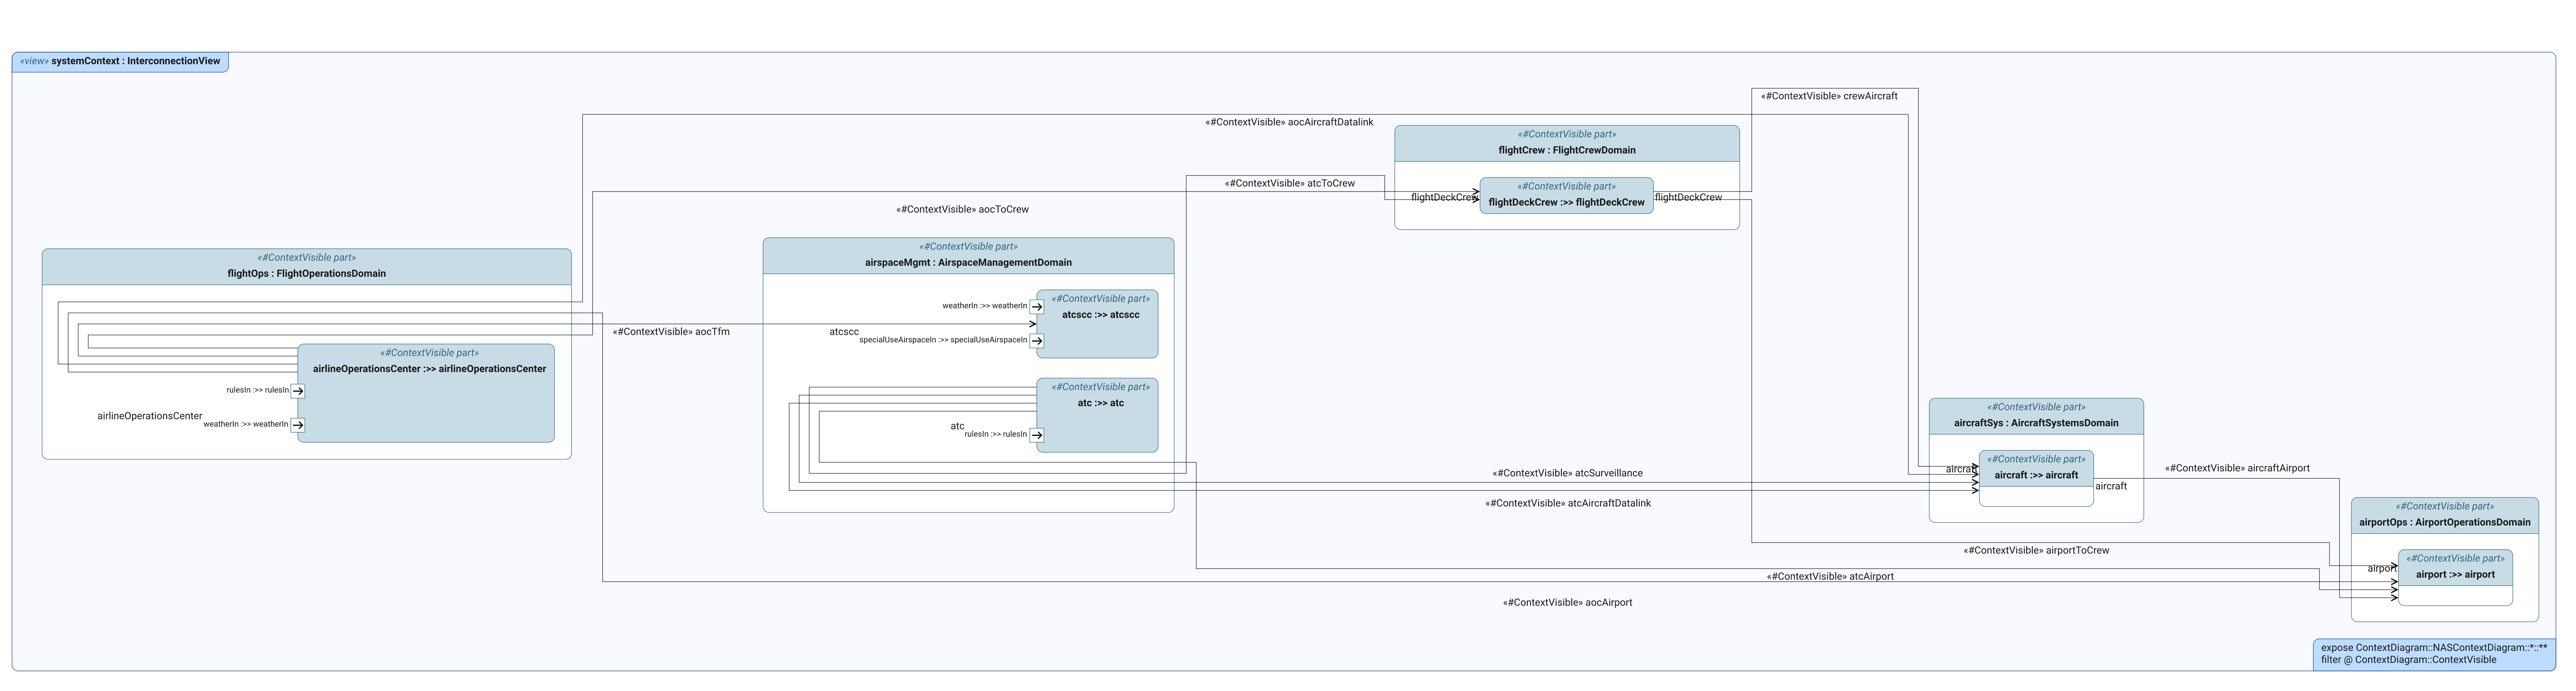
\includegraphics[width=\linewidth,height=0.8\textheight,keepaspectratio]{sysml/diagram-systemContext}
\caption{NAS context diagram. View \texttt{systemContext}; source \texttt{nas\_context\_diagram.sysml}; rendered 2026-10-10.}
\label{fig:sysml-systemContext}
\end{figure}
\end{landscape}


\subsection{Stakeholder Objectives}
\label{sec:objectives-results}

% Drafted 2026-10-11 for the owner's note "DO" (print page 17) as a subsection of
% Results; moved here 2026-10-13 (owner's note, print page 26: "Move to earlier
% section that discusses objectives?"). It follows Scope because it speaks only
% of the stakeholders and objectives kept there.
\aidraft{What ``optimal'' means to each stakeholder, and where the objectives conflict (your note: ``DO''). Source: the synthesis section of \texttt{knowledge/models/stakeholder-objective-ontology.md}, whose own status note says the classifications are judgment calls not yet sourced from annotated literature. Limited here to the stakeholders and objectives kept in Section~\ref{sec:scope}.}
Each stakeholder kept in scope pursues a different objective when an aircraft's trajectory is changed. The airline wants the lowest cost for its flights, which combines fuel, time, and the consequences of a late arrival for connecting passengers. Air traffic control wants separation assured with a workload the sector team can sustain, and a traffic picture that stays predictable. The flight crew wants instructions the aircraft can fly, given with enough time to set them up.

Some of these objectives align. Burning less fuel lowers the airline's cost and lowers carbon dioxide emissions together. Air traffic control's wish for predictability and the airline's wish to keep its schedule both favor aircraft that fly what was planned.

Others conflict, and the conflict this project studies is the first of them: the trajectory that is cheapest for one aircraft is not always the one that costs the sector least to grant. A request or a resolution that saves fuel for one flight can add instructions, monitoring, and follow-up for the controller. That cost is externalized. It does not appear in the airline's own cost function, and the party that bears it has no means to price it back.

The objectives also operate on different timescales. An airline sets its schedule policy over months, realizes fuel cost per flight, and realizes delay cost in minutes. Air traffic control manages capacity over years through sector design and over seconds through tactical control. A decision made in minutes by one party is judged against objectives the others hold on other clocks.
% ---- end AI draft

\subsection{Project Deliverables}
\label{sec:deliverables}

\plantodo{S10, S14, S16}{State the goals and deliverables: the SysML reference architecture, the traceability chain from stakeholder needs to aircraft-level behavior, and the experiment (Section~\ref{sec:experiment}). Include the quantifiable measures used to assess success (e.g., traceability coverage, stakeholder coverage, demonstration of a local-vs-SoS tradeoff).}

% Owner's note, 2026-10-13 print, page 13: the two sentences that stood here are
% struck; beside them "Context, [bdd], ibd, activities, requirements, experiment &
% traceability chain & gap analysis. Have Claude propose a table."
\aidraft{Proposed deliverables table (your note: ``Have Claude propose a table''). The eight rows are your list; Claude read its second word as ``bdd''. The middle and right columns are Claude's proposal. No block definition diagram or requirements view is rendered yet, and the trace table and the gap analysis are not written: the table says where each will go, not that it is there.}
The project delivers the eight items of Table~\ref{tab:deliverables}.

\begin{table}[htbp]
\centering
\small
\caption{Project deliverables.}
\label{tab:deliverables}
\begin{tabular}{@{}p{3.6cm}p{7.6cm}p{3.6cm}@{}}
\toprule
Deliverable & What it shows & Where in this report \\
\midrule
Context diagram & The systems kept in the System of Interest, the actors at its boundary, and the exchanges among them & Section~\ref{sec:scope} \\
Block definition diagrams & The NAS broken down into domains and constituent systems & Appendix~\ref{app:architecture} \\
Internal block diagrams & The parts inside the aircraft and inside airspace management, and the links among them & Section~\ref{sec:architecture-results} \\
Activity diagrams & One nominal flight from gate to gate, and the place of the conflict within it & Section~\ref{sec:conops-results} \\
Requirements & Stakeholder requirements, system requirements and constituent-system requirements, each traced to the tier above & Appendix~\ref{app:architecture} \\
Experiment & One conflict resolved four ways and scored for the aircraft, the airline, the sector and the system & Sections~\ref{sec:experiment} and~\ref{sec:experiment-results} \\
Traceability chain & One thread from the airline's cost objective through the requirements and the airline-to-ATC interface to the experiment's outcome table & Section~\ref{sec:experiment-results}; Appendix~\ref{app:architecture} \\
Gap analysis & The requirements that today's NAS does not meet, and what the experiment measures for each & Section~\ref{sec:results} \\
\bottomrule
\end{tabular}
\end{table}
% ---- end AI draft

\subsection{Project Timing}
\label{sec:timing}

\plantodo{S1 (new)}{Revisit the timeline from the 503 Proposal submittal (see \texttt{prework/ISD 503 Submittal.pdf}) and show the plan now in force: the nine one-week turns of D-016 (the table at the top of \texttt{to-do-list.md}), each with its exit test and target date, next to the August milestones in Table~\ref{tab:project-timing}.}

% Table moved here from Project Deliverables and given a Status column,
% 2026-10-13 (owner's note, print page 14: "Old plan presented for reference.
% Disposition each's status w/ not started, draft, complete, or will not
% implement."). The status of each row is the owner's handwriting beside it. The
% print has no mark beside the last three rows: "Not started" on the last two is
% Claude's entry, and the row before them is left empty for the owner.
The plan established at the project's inception is presented in Table~\ref{tab:project-timing} for reference, with the status of each item: not started, draft, complete, or will not implement.

\begin{table}[htbp]
\centering
\small
\caption{Project milestones and verification methods of the original plan, with the status of each.}
\label{tab:project-timing}
\begin{tabular}{|p{0.15\textwidth}|p{0.15\textwidth}|p{0.12\textwidth}|p{0.11\textwidth}|p{0.17\textwidth}|p{0.11\textwidth}|}
\hline
\textbf{Project Milestone} & \textbf{Deliverable} & \textbf{Lead/Team Member} & \textbf{Expected Completion Date} & \textbf{Target Metric/Verification Method} & \textbf{Status} \\
\hline
Literature Review & Annotated bibliography & Owen & 9/7/2026 & 10--20 papers categorized & Draft \\
\hline
PESTLE Analysis \& Systems-of-Interest Definition & Context diagram, text-based documentation & Owen & 9/10/2026 & Review & Complete \\
\hline
Systems-of-Interest Definition & Text-based documentation & Owen & 9/15/2026 & Clear boundaries and exclusions & Complete \\
\hline
Operational Scenarios & ConOps document & Owen & 9/22/2026 & 1--3 representative scenarios & Draft \\
\hline
Draft Architecture & BDDs and package structure & Owen & 10/1/2026 & All domains represented & Complete \\
\hline
Interface Definition & Interface Control Document & Owen & 10/12/2026 & All interfaces identified & Draft \\
\hline
Internal Block Diagrams & IBDs & Owen & 10/17/2026 & Critical interfaces connected & Draft \\
\hline
Requirements Definition & Requirements model & Owen & 10/20/2026 & Trace to stakeholders & Draft \\
\hline
Measures of Effectiveness & MOE/MOP hierarchy & Owen & 10/25/2026 & Quantifiable metrics defined & Complete \\
\hline
Requirement Traceability & Requirements matrix & Owen & 10/29/2026 & Complete allocation & Draft \\
\hline
Activity Diagrams & Operational activities & Owen & 11/3/2026 & Scenario walkthrough & Draft \\
\hline
Sequence Diagrams & Information exchanges & Owen & 11/8/2026 & Message completeness & Not started \\
\hline
State Machines & State behavior of key entities & Owen & 11/13/2026 & Executable state logic & Will not implement \\
\hline
Authority \& Responsibility Models & RACII (Responsible, Accountable, Consulted, Informed) & Owen & 11/17/2026 & All decisions assigned & Will not implement \\
\hline
Optimization Prototype & Working code & Owen & 11/21/2026 & Unit test cases & Draft \\
\hline
Integration into MBSE Architecture & Traceability links & Owen & 11/24/2026 & End-to-end scenario & \\
\hline
Final Baseline \& Final Paper & Versioned model \& thesis/paper & Owen & 12/16/2026 & Draft & Not started \\
\hline
Paper Submittal & Thesis/paper & Owen & 12/20/2026 & Official submittal & Not started \\
\hline
\end{tabular}
\end{table}

% Keeps the two tables above inside Section 1 (placeins, loaded in main.tex).
\FloatBarrier

% !TEX root = ../main.tex
\section{Assumptions and Methodology}
\label{sec:methodology}

% Revised 2026-10-11 from the owner's hand review of the printed report
% (handwritten/2026-10-11_main.md, notes 10.x to 12.x). The experiment design and
% the scoring calculations moved to sections/04_experiment.tex. "The Two Claims"
% is no longer a subsection: its call-out is at the top of 02_introduction.tex.
% The owner's paragraphs were edited for spelling and sentence sense at the
% owner's request; passages between \aidraft{...} and "% ---- end AI draft" were
% drafted by Claude and are the owner's to rewrite.
% Revised again 2026-10-13 from the second print (handwritten/2026-10-13_main.md,
% notes 13.x to 17.x).

The problem is that the inertia of past, piecemeal designs and the high cost of upgrading the NAS make the system hard to change. The project proposes a new airline-to-ATC interface and a new way of deciding which aircraft to move in a conflict, which together could lower the cost of air traffic management.

\plantodo{Track C (owner's note, 2026-10-13 print, page 13)}{\textbf{``Expand upon.''} The paragraph above is bracketed with this note. Not drafted by Claude: no source in \texttt{evidence/source-register.md} has been read for the inertia of past designs or the cost of upgrading the NAS, so the expansion is yours, or name the source and it can be read first.}

Toward those ends, the project uses a model-based systems engineering (MBSE) approach to design the architecture and the decision-making process, and a simulation-based experiment to test the proposed interface and decision-making process. First, a literature review was conducted to:
\begin{enumerate}
    \item identify the current state of air traffic management,
    \item identify the relevant stakeholders and their objectives,
    \item identify the requirements necessary to meet those objectives, and
    \item identify the gaps in the current system that the proposed interface and decision-making process can address.
\end{enumerate}

\subsection{Systems Engineering Approach}
\label{sec:se-approach}

Standard systems engineering methods of analysis and decomposition were applied to the collected evidence, which produced a context diagram, internal block diagrams, and activity and sequence views. These identified the relevant systems and the interactions among them that are necessary to meet the stakeholders' objectives. From them the stakeholder requirements were written and then decomposed into system-level requirements (SLRs) for the NAS. The SLRs were allocated to the relevant constituent systems, and high-level requirements (HLRs) decomposed them one level further.

This enabled the project to (1) build a model of the architecture and the decision-making process, and (2) compare current air traffic management practice, which relies on general rules of thumb and knowledge of what has worked before~\cite{rantanen2012conflictManeuvers,kirwan2001coraStrategies}, with a model-based decision-support approach that replaces the low-fidelity decision rule with one or more higher-fidelity models of aircraft performance, at varying levels of accuracy and information.

The emphasis is on structure, behavior, interfaces, and traceability, not on optimization mathematics. The project's commercial value to the author lies in a better understanding of the systems, their interactions, and the divisions of responsibility that inhibit information flow and lead to sub-optimal outcomes. To explore that in a meaningful way, decision support and optimization are treated as a capability inside the architecture, which following MBSE principles makes possible.

\aidraft{The two paragraphs below are yours, reworded by Claude for your note ``Reword'' on the 2026-10-13 print (page 15). The claims are unchanged; your originals are in git history (commit 965f5d5).}
The systems and their constituent systems could be documented in more detail (examples are in Appendix~\ref{app:architecture}), and more formal mathematical models could be used. Neither was needed to deliver the project's commercial value to its customer, so neither was done. The project's artifacts were tailored to the customer's needs, as customer-focused MBSE calls for.

The steps of the process were tailored in the same way, to the time the author had available. The literature review began as one pass and then continued as the work required. The gate-to-gate concept of operations was written informally and refined with publicly available general knowledge of the NAS. No alternative system decomposition was formally explored beyond the initial abstraction decisions. The ISO/IEC/IEEE 15288 technical processes were followed in this tailored form, which the standard provides for.
% ---- end AI draft

Table~\ref{tab:se-processes} summarizes the systems engineering processes and the artifacts that realize them.

\begin{table}[h]
\centering
\small
\caption{Systems engineering processes and the artifacts that realize them.}
\label{tab:se-processes}
\begin{tabular}{@{}p{4.2cm}p{6.2cm}p{4.6cm}@{}}
\toprule
Process (15288 / INCOSE) & Artifact in this project & Where \\
\midrule
Stakeholder needs and requirements & 13 stakeholder requirements, each traced to an objective row & \texttt{requirements\_stakeholders.sysml}; Appendix~\ref{app:architecture} \\
System requirements & 23 system requirements, allocated to constituent systems; 28 constituent-system requirements one tier down & \texttt{requirements\_nas\_system.sysml}; \texttt{requirements\_constituent\_systems.sysml} \\
Architecture definition & Context diagram, internal block diagrams, typed interfaces on the thread, activity and sequence views & \texttt{cameo\_models/}; Section~\ref{sec:architecture-results} \\
System analysis & Experiment at three fidelities, outcome table & \texttt{simulation/}; Sections~\ref{sec:experiment} and~\ref{sec:experiment-results} \\
Verification & Verification cases for the improved requirements, run by the experiment & \texttt{nas\_verification.sysml} \\
Validation & Stakeholder-level reading of the outcome table (who pays) with MoEs or MoPs & Section~\ref{sec:results} \\
\bottomrule
\end{tabular}
\end{table}

% Removed 2026-10-13 as the owner marked on the print, page 15 and 16: the call-out
% asking for the 15288 process names to be checked (scribbled over; the check
% itself has not been done), the last three rows of the table ("Remove these 3."),
% the MBSE-methodology call-out ("Done") and the decomposition call-out ("WNI",
% will not implement).

\subsection{Working Assumptions}
\label{sec:assumptions}

The working assumptions fall into two groups: assumptions about the problem and its context, and assumptions about the methodology.

The problem statement assumes that:
\begin{itemize}
    \item the abstractions used in the model are sufficient to capture the relevant behavior of the system;
    \item the stakeholders' objectives are comprehensively captured and accurately represented in the model;
    \item the scenario is sufficient to explore the potential benefit of interconnected MBSE.
\end{itemize}

Every abstraction was made with the express goal of capturing the relevant behavior of the system, as defined by the stakeholders' objectives. The System of Interest, the NAS as a system of systems, was ratified around the trajectory-intent lifecycle, from enterprise objectives through aircraft motion. An entity is modeled when it has distinct decision authority or execution behavior that is dynamically coupled to in-scope decisions and materially affects cost, safety, workload, schedule reliability, or passenger value. Boundary actors supply objectives, demand, feedback, or rules without being decomposed as decision mechanisms. Exogenous influences enter as constraints or scenario parameters. This criterion preserves the authority and responsibility relationships a system-of-systems architecture needs without expanding the project into a model of every NAS participant.

The methodology assumes that:
\begin{itemize}
    \item models of every required aircraft type are available;
    \item the security concerns of sharing airline data can be mitigated;
    \item the proposed interface can be implemented in the NAS over digital communication channels between the airline and ATC, between the aircraft and ATC, or both;
    \item the airline reports its weight and cost index accurately;
    \item the conflict can be treated as a snapshot, with the traffic unchanged while the decision is made;
    \item the specific scenario presented in the experiment is representative of a larger set of scenarios that generalize to the NAS as a whole.
\end{itemize}

\plantodo{Track C (owner's note, 2026-10-13 print, page 16)}{Beside the interface and communication-channel assumptions, now one item: \textbf{``Combine. Later cite EPP, value for [CI/GW], BADA4 for API models?''} ``CI/GW'' (cost index and gross weight) is Claude's reading of the handwriting. BADA 4 is not in \texttt{evidence/source-register.md}.}

% The list of limits that stood here (AI-drafted 2026-10-11) is taken apart as
% the owner marked on the 2026-10-13 print, pages 16 and 17: its lead-in sentence
% is struck; the static-snapshot and truthful-reporting items are reworded into
% the list above ("reword & add to primary list"; "Accurate info. Move to primary
% list."); the first two items are discussion ("Add to discussion instead of the
% list."); the climb rule now cites its source ("Cite source."); the sentence on
% the aircraft model's simplifications sits with the accuracy item ("Move to
% discussion regarding accuracy bullet, above."). The call-out asking for a
% source for a 1 to 3 percent misreporting figure is removed (scribbled over).
The scenario stands for a narrow set of conflicts. Conflicts between two aircraft crossing at the same level are a minority of conflicts: 36 of 256 in the operational data of \textcite{rantanen2012conflictManeuvers}. The experiment uses one invented en-route sector and four aircraft. The rule that limits climbs when the weight is unknown is a single threshold (FL350) applied to every aircraft type; it is the modeling assumption of an earlier study, which limited climbs in that way because it did not model aircraft weight~\cite{engility2014tasarAlaska}.

The assumption of accurate information has two parts. An airline could misreport what it shares. The aircraft performance model that turns the shared weight into a cost is itself simplified, and its simplifications are listed separately in Section~\ref{sec:scoring-limits}.

\aidraft{One sentence offered for the misreporting point, not asked for on the print. The source was read in full by Claude on 2026-10-11 and not by you; it concerns flow programs before departure, not a conflict in cruise. Keep it, or strike it.}
The risk is documented for a related exchange: where an airline states the relative cost of its route options to the FAA's flow-management automation, the airline would reduce its delays by stating a very high cost~\cite{kulkarni2019ctopSlotSubstitution}.
% ---- end AI draft

\subsection{Proposed Airline-to-ATC Interface}
\label{sec:proposed-interface}

\plantodo{Track C (owner's question, 2026-10-13 print, page 17)}{\textbf{``This shouldn't be its own section here. Where would this fit?''} Not moved; the choice is yours. Claude's suggestion: the proposal is a result of the architecture work, so put it in Section~\ref{sec:architecture-results} as the improved architecture, next to the baseline diagrams, and leave one sentence in Section~\ref{sec:experiment-method} that says cases C and D use it. The other candidate is Section~\ref{sec:experiment-method} itself, which keeps it ahead of the experiment that depends on it.}

\plantodo{Track C (D-019)}{\textbf{Name the digital-thread artifact.} Describe \texttt{AirlinePerformanceShare}: what it carries (gross weight, cost index, connection priority; thrust, drag and fuel-flow model identifiers present but not exercised), who sends it (airline operations center or FMS), who receives it (ATC decision support, per D-012 owned by the system that decides), and which requirements it satisfies (SLR-INF-02) and the goal it serves (SLR-CLR-13). State that security is an assumption. \textbf{Owner's note, 2026-10-11 print: ``important to do''} --- position it against ADS-C EPP and Coppenbarger's Table 2 (the same items, a different receiver); a first draft of that positioning follows.}

% The AI-DRAFTED call-out that stood here is removed (scribbled over on the
% 2026-10-13 print, page 17); the owner's edits to the two paragraphs are applied.
% Still true of the second sentence: the ADS-C EPP statement rests on
% sesarju2019solutionsCatalogue, registered from its title page and contents only.
The items the interface carries are not new. \textcite{coppenbarger1999climbPrediction} listed take-off weight, thrust and drag factors, and the speed profile as candidates for exchange between an airline and air traffic control, and measured what airline-supplied weight does for the prediction of a climb. In Europe, the Extended Projected Profile is sent over ADS-C to downlink the trajectory that the flight management system predicts~\cite{sesarju2019solutionsCatalogue}. What has kept the items out of use is ownership, not feasibility: weight and speed intent ``are considered competitive parameters by airlines and are not available for use''~\cite{schultz2012adaptiveClimb}. A second obstacle is the availability of first-principles data for each aircraft type: thrust, drag and fuel flow.

The proposal here keeps the items and changes the receiver and the purpose. In the earlier work the data feeds a trajectory predictor, to make the prediction of one aircraft's flight path more accurate. Here it feeds the decision support of the party that chooses which aircraft to move, to change the choice. This provides for asking ``what if'' within a mathematical framework. The interface is typed in the model, tagged as part of the improved architecture, and tied to the requirement it satisfies, so the report can point at a model element where the earlier work has a finding in prose. Confidentiality is stated as an assumption: the data is disclosed only to the deciding party, and no security mechanism is modeled.

% !TEX root = ../main.tex
\section{System Model}
\label{sec:system-model}

% New section, 2026-10-17, at the owner's request: the systems engineering work
% gets its own section between the methodology and the experiment (D-028). Built
% from blocks moved whole, with their markers and source comments:
%   Stakeholders            <- 02_introduction.tex: Stakeholder Selection, the
%                              de-scoping part of Scope, Stakeholder Objectives
%   Constituent Systems     <- 02_introduction.tex: System Identification and Selection
%   System of Interest      <- 02_introduction.tex: the end of Scope and the context diagram
%   Operational Concept     <- 05_results_discussion.tex (now 06_)
%   Architecture            <- 05_results_discussion.tex (now 06_)
%   Proposed Airline-to-ATC Interface <- 03_assumptions_methodology.tex
% The Introduction keeps a short summary (Stakeholders and Study Boundary) that
% points here. The subsections run in order: who has a stake, what they want and
% where they conflict, which systems act, the boundary studied, how it operates,
% the architecture, and the interface the experiment tests.

\aidraft{Section opener, written 2026-10-17 for the new section. Replace with your own.}
This section presents the model the experiment is built on. It begins with the stakeholders, their objectives and the conflict among them, identifies the constituent systems through which they act, and draws the boundary of the System of Interest. It then describes how a flight operates within that boundary, the architecture that carries it, and the airline-to-ATC interface whose value the experiment of Section~\ref{sec:experiment} measures.
% ---- end AI draft

\subsection{Stakeholders}
\label{sec:stakeholders}

\subsubsection{Identification}

% Moved from the Introduction's Stakeholder Selection subsection, 2026-10-17.
Informed by the literature survey and the author's experience in the aviation industry, a set of candidate stakeholders was identified and refined using a PESTLE analysis and stakeholder discovery process. The result is a diverse group of stakeholders that represent the various interests and perspectives affected by NAS operational decisions, and is shown in Figures~\ref{fig:stakeholders-exploration} and~\ref{fig:stakeholders-power-interest}. The stakeholders are grouped by the six domains of a PESTLE analysis (political, economic, social, technological, legal, environmental) and scored for importance and impact on trajectory decisions. The assessment is documented in the \texttt{capstone\_stakeholder\_assessment.xlsx} file, along with an initial assessment of each candidate stakeholder's objectives, candidate MOPs and MOEs, and whether the stakeholder has a direct or indirect effect on trajectory decisions. The assessment also considers whether the stakeholder should stand alone or be abstracted through consolidation with another, and the reason for that decision. An excerpt of the work is in Appendix~\ref{app:stakeholders}, Table~\ref{tab:stakeholder-assessment-excerpt}.

\begin{figure}[htbp]
\centering
\figorbox{stakeholders_exploration.png}{MISSING: \texttt{report/figures/stakeholders\_exploration.png}}
\caption{Candidate stakeholders of the NAS as a system of systems.}
\label{fig:stakeholders-exploration}
\end{figure}

\begin{figure}[htbp]
\centering
\figorbox{stakeholders_impact_power_exploration.png}{MISSING: \texttt{report/figures/stakeholders\_impact\_power\_exploration.png}}
\caption{Candidate stakeholders placed by power and interest.}
\label{fig:stakeholders-power-interest}
\end{figure}
The power analysis informed the decision to keep four stakeholders in scope: the airline, air traffic control, the airport authority, and the flight crew. The other stakeholders are treated as boundary actors that supply rules, equipment, demand, and expectations to the decision but do not make it or execute it. The four kept stakeholders appear on the context diagram (Figure~\ref{fig:sysml-systemContext}) and are decomposed in the model.

\subsubsection{Candidate Objectives}

An exploration of each stakeholder's interests led to the following list of objectives relevant to the project:

% The descriptions were added 2026-10-17 at the owner's request ("add a brief
% description of the objectives to clarify what they are and why they're
% objectives"); the twelve names are the owner's list, unchanged.
\aidraft{One-line description of each objective: what it means in the NAS and which stakeholder holds it. Drawn from the per-stakeholder tables in \texttt{knowledge/models/stakeholder-objective-ontology.md} and the assessment spreadsheet; that file's own status note says its classifications are judgment calls not yet sourced from annotated literature, so these descriptions are too. The opening sentence on why each is an objective is Claude's.}
Each item is an objective because at least one stakeholder seeks to raise or lower it, and it can be measured, as a measure of performance for one system or a measure of effectiveness for the whole.
\begin{description}
    \item[Safety / Security] Keeping aircraft separated from each other, from terrain and from hazardous weather, and protecting the operation from deliberate harm. Held by every stakeholder; for air traffic control and the flight crew it is a constraint that is never traded.
    \item[Efficiency] Flying the flight with the least fuel and time for the distance covered. Held by the airline, whose fuel cost depends directly on the trajectory flown.
    \item[Throughput / Capacity] The number of aircraft a sector, runway or airport can handle in a period. Held by air traffic control and the airport authority.
    \item[Reliability / Resilience] The ability of the operation to run as planned and to recover when it is disrupted. Held by the airline and by air traffic control.
    \item[Environmental Impact] The carbon dioxide, other emissions and contrails a flight produces, which follow from the fuel it burns and the path it flies. Held by environmental and societal organizations and, through regulation, by governments.
    \item[Noise Impact] Sound over the communities near airports, set by the departure and approach paths. Held by communities and the airport authority.
    \item[Passenger Satisfaction] The passenger's experience of travel time, comfort and connections. Held by passengers, and by the airline through the revenue that follows.
    \item[Schedule Reliability] Arriving on time and keeping passengers' connections. Held by the airline and its passengers.
    \item[Cost / Profitability] The operator's cost of a flight (fuel, crew, the consequences of delay) and the profit it supports. Held by the airline and its investors.
    \item[Maintenance / Lifecycle Cost] The upkeep of aircraft and engines over their life. Held by the operator and the manufacturers.
    \item[Regulatory Compliance] Operating within the rules, procedures and clearances in force. Held by the flight crew and the airline, and enforced by the regulators.
    \item[Workload / Human Factors] The mental and procedural demand on controllers, dispatchers and crews. Held by air traffic control and the flight crew, for whom high workload is a cost and a source of error.
\end{description}
% ---- end AI draft
These objectives were then assessed for relevance to the decision under study, and six were kept: safety, efficiency, environmental impact, schedule reliability, cost, and workload. The other objectives were set aside for the reasons given in Section~\ref{sec:scope}.

\subsubsection{Selection}
\label{sec:scope}

% Moved 2026-10-17 from the Introduction's Scope subsection (the label sec:scope
% moved with it, so references to the de-scoping reasons still resolve). The
% closing sentence and the context diagram went to System of Interest below. One
% edit to the first sentence: it named the stakeholder and system subsections as
% coming before it; the systems now come after.
% Owner's note, 2026-10-11 print, page 7: "Leave larger list above, discuss
% de-scoping decisions here & include the final list/diagram." The strikes and
% margin notes on page 6 are the content below. Revised 2026-10-13 from the
% second print, pages 10 and 11: the kept stakeholders are named as on the context
% diagram, the reasons for profitability, reliability, maintenance and lifecycle
% cost and for throughput and capacity are the owner's handwritten ones, and the
% throughput call-out the owner scribbled over is removed.

\aidraft{De-scoping decisions and the final lists (owner's note: ``Leave larger list above, discuss de-scoping decisions here and include the final list/diagram''). The reasons in quotation marks are your margin notes. On the 2026-10-13 print you supplied the reasons for profitability, reliability, maintenance and lifecycle cost, and throughput and capacity; they are below in your words. Still Claude's reading, not yours: the reason given for the four stakeholders, and the reason given for security, resilience and regulatory compliance.}
The stakeholders and objectives above are the result of exploration. The study itself is narrower. It examines one tactical decision, the resolution of a conflict between aircraft in cruise, and keeps only the stakeholders and objectives that bear on that decision.

Four stakeholders remain, together with the aircraft, and each appears on the context diagram (Figure~\ref{fig:sysml-systemContext}): operators, as flight operations and its airline operations center; air traffic control, within airspace management; the airport authority, as airport operations; and the flight crew. The aircraft appears as aircraft systems. Governments and standards organizations, aircraft and engine manufacturers, passengers, and environmental and societal organizations are outside the System of Interest. They supply rules, equipment, demand, and expectations to the decision but do not make it or execute it, so they are treated as boundary actors and not decomposed.

Six stakeholder objectives remain: safety, efficiency, environmental impact, schedule reliability, cost, and workload. Schedule reliability is carried in the experiment as a step in cost when a flight's delay passes a threshold (the parameter $K$ of Section~\ref{sec:scoring-method}). The others were set aside for the following reasons. Noise impact: the measure is ``not relevant at cruise.'' Passenger satisfaction: ``not measurable objectively.'' Profitability falls out of the other objectives; it is tracked at the operator's organizational level and is more complex than any one decision. Reliability is captured with schedule reliability. Maintenance and lifecycle cost are largely determined by the number of flight cycles, the chosen takeoff performance, the flight distance and the climb controls, so one air traffic control decision has a negligible effect on them. Security, resilience and regulatory compliance are not changed by the choice between resolution options in the scenario. Throughput and capacity were left for another study. They are also close to ongoing work by the author, and out of an abundance of caution that part of the problem space was avoided.
% ---- end AI draft

\subsubsection{Objectives and Conflicts}
\label{sec:objectives-results}

% Drafted 2026-10-11 for the owner's note "DO" (print page 17) as a subsection of
% Results; moved to the Introduction 2026-10-13 (owner's note, print page 26: "Move
% to earlier section that discusses objectives?"); moved here 2026-10-17 as the
% close of Stakeholders, at the owner's suggestion. It follows Selection because it
% speaks only of the stakeholders and objectives kept there.
\aidraft{What ``optimal'' means to each stakeholder, and where the objectives conflict (your note: ``DO''). Source: the synthesis section of \texttt{knowledge/models/stakeholder-objective-ontology.md}, whose own status note says the classifications are judgment calls not yet sourced from annotated literature. Limited here to the stakeholders and objectives kept in Section~\ref{sec:scope}.}
Each stakeholder kept in scope pursues a different objective when an aircraft's trajectory is changed. The airline wants the lowest cost for its flights, which combines fuel, time, and the consequences of a late arrival for connecting passengers. Air traffic control wants separation assured with a workload the sector team can sustain, and a traffic picture that stays predictable. The flight crew wants instructions the aircraft can fly, given with enough time to set them up.

Some of these objectives align. Burning less fuel lowers the airline's cost and lowers carbon dioxide emissions together. Air traffic control's wish for predictability and the airline's wish to keep its schedule both favor aircraft that fly what was planned.

Others conflict, and the conflict this project studies is the first of them: the trajectory that is cheapest for one aircraft is not always the one that costs the sector least to grant. A request or a resolution that saves fuel for one flight can add instructions, monitoring, and follow-up for the controller. That cost is externalized. It does not appear in the airline's own cost function, and the party that bears it has no means to price it back.

The objectives also operate on different timescales. An airline sets its schedule policy over months, realizes fuel cost per flight, and realizes delay cost in minutes. Air traffic control manages capacity over years through sector design and over seconds through tactical control. A decision made in minutes by one party is judged against objectives the others hold on other clocks.
% ---- end AI draft

% Where to put the stakeholder requirements?

\subsection{Constituent Systems}
\label{sec:systems-selection}

% Was "System Identification and Selection" in the Introduction (made 2026-10-13
% from the owner's note on Figure 3, print page 9: "These are systems, not
% stakeholders. Move! 'System Identification & Selection'?"). Moved here and
% renamed 2026-10-17. The transition and the paragraph on the figure were added
% at the owner's request ("add a nice transition from the stakeholder work ...
% discuss the broad theorization reflected in the Miro board").
\aidraft{Transition from the stakeholder work, and a reading of the Miro board in Figure~\ref{fig:sos-exploration}. The description of the figure is Claude's reading of the exported image; the rationale the board reflects is the owner's and is only partly written down in the repository, so check each claim about why the board is drawn as it is.}
Stakeholders do not change a trajectory themselves. They act through systems: a controller through the sector's displays and radios, an airline through its operations center and dispatch tools, a crew through the flight deck and the flight management system. And the cost of whatever they decide is realized in one place, the aircraft, as fuel burned and time flown. The constituent systems through which the stakeholders act were therefore identified next.

Figure~\ref{fig:sos-exploration} places the NAS at the center and branches outward to the systems that could act on a flight: the aircraft, air traffic control, operators, airports, maintenance suppliers, communication, the regulatory bodies, and passengers. The board is deliberately broad. It follows the system-of-systems view quoted in Section~\ref{sec:introduction}, of many heterogeneous systems at several levels, and lists every system that could bear on a flight before any is set aside. Air traffic control divides into the air navigation service providers, whose terminal and en-route facilities control individual flights, and the national command center, whose traffic management units and flow programs shape demand across many. Operators divide into general aviation, airlines and militaries; within the airline, the operations center and its dispatchers sit beside the business, pilots, ticketing and IT functions.

The board decomposes its branches in two different ways, and the difference reflects the problem the project studies. The organizations that decide, air traffic control and the airline, are broken down to the people who make the decision: the individual controller and the dispatcher. The aircraft is broken down to the physical systems that carry it out: the flight management system's guidance and navigation functions, the propulsion components and the fuel system. The decision about a trajectory is made in one part of the system of systems, and its cost is realized in another.
% ---- end AI draft

\plantodo{Track C (owner's request, 2026-10-17)}{\textbf{Your experience behind the board.} Add what your experience in the FMS industry contributed to Figure~\ref{fig:sos-exploration} (an [SME] statement): for example, why the flight management system is decomposed to its functions, and which parts of the board came from that experience rather than from the literature of Section~\ref{sec:litreview}. Name any source the board drew on so it can be cited here.}

The aircraft is treated alongside the stakeholders as a constituent system. Figure~\ref{fig:sos-exploration} shows the systems first identified within the NAS, with the aircraft decomposed furthest, as its systems and their performance dictate the cost of each flight.

\begin{figure}[htbp]
\centering
\figorbox[\textwidth]{system_of_systems_detailed_exploration.png}{MISSING: \texttt{report/figures/system\_of\_systems\_detailed\_exploration.png}}
\caption{The NAS as a system of systems: candidate constituent systems.}
\label{fig:sos-exploration}
\end{figure}

\subsection{System of Interest}
\label{sec:soi}

% Made 2026-10-17. The closing sentence of the old Scope draft and the context
% diagram moved here from the Introduction.
\aidraft{Two connecting sentences, written 2026-10-17. They restate the selection of Section~\ref{sec:scope}; replace with your own.}
The System of Interest is drawn from the systems of Figure~\ref{fig:sos-exploration}: the systems operated by the four stakeholders kept in Section~\ref{sec:scope}, and the aircraft. The systems of the boundary actors are not decomposed; they appear only through what they supply to the decision.

Figure~\ref{fig:sysml-systemContext} is the resulting System of Interest as modeled: the constituent systems kept and the exchanges among them.
% ---- end AI draft

% GENERATED by tools/render_sysml_diagrams.py. Do not edit: the next run overwrites it.
% To change a caption, edit the `// caption:` line above the view in the .sysml file.
% To add or remove a figure, add or remove the view in the model.
% To move a figure between the body and the appendix, add or remove a
% `// placement: body` line above the caption line.

\begin{landscape}
\begin{figure}[!htbp]
\centering
\pdfimageresolution=300
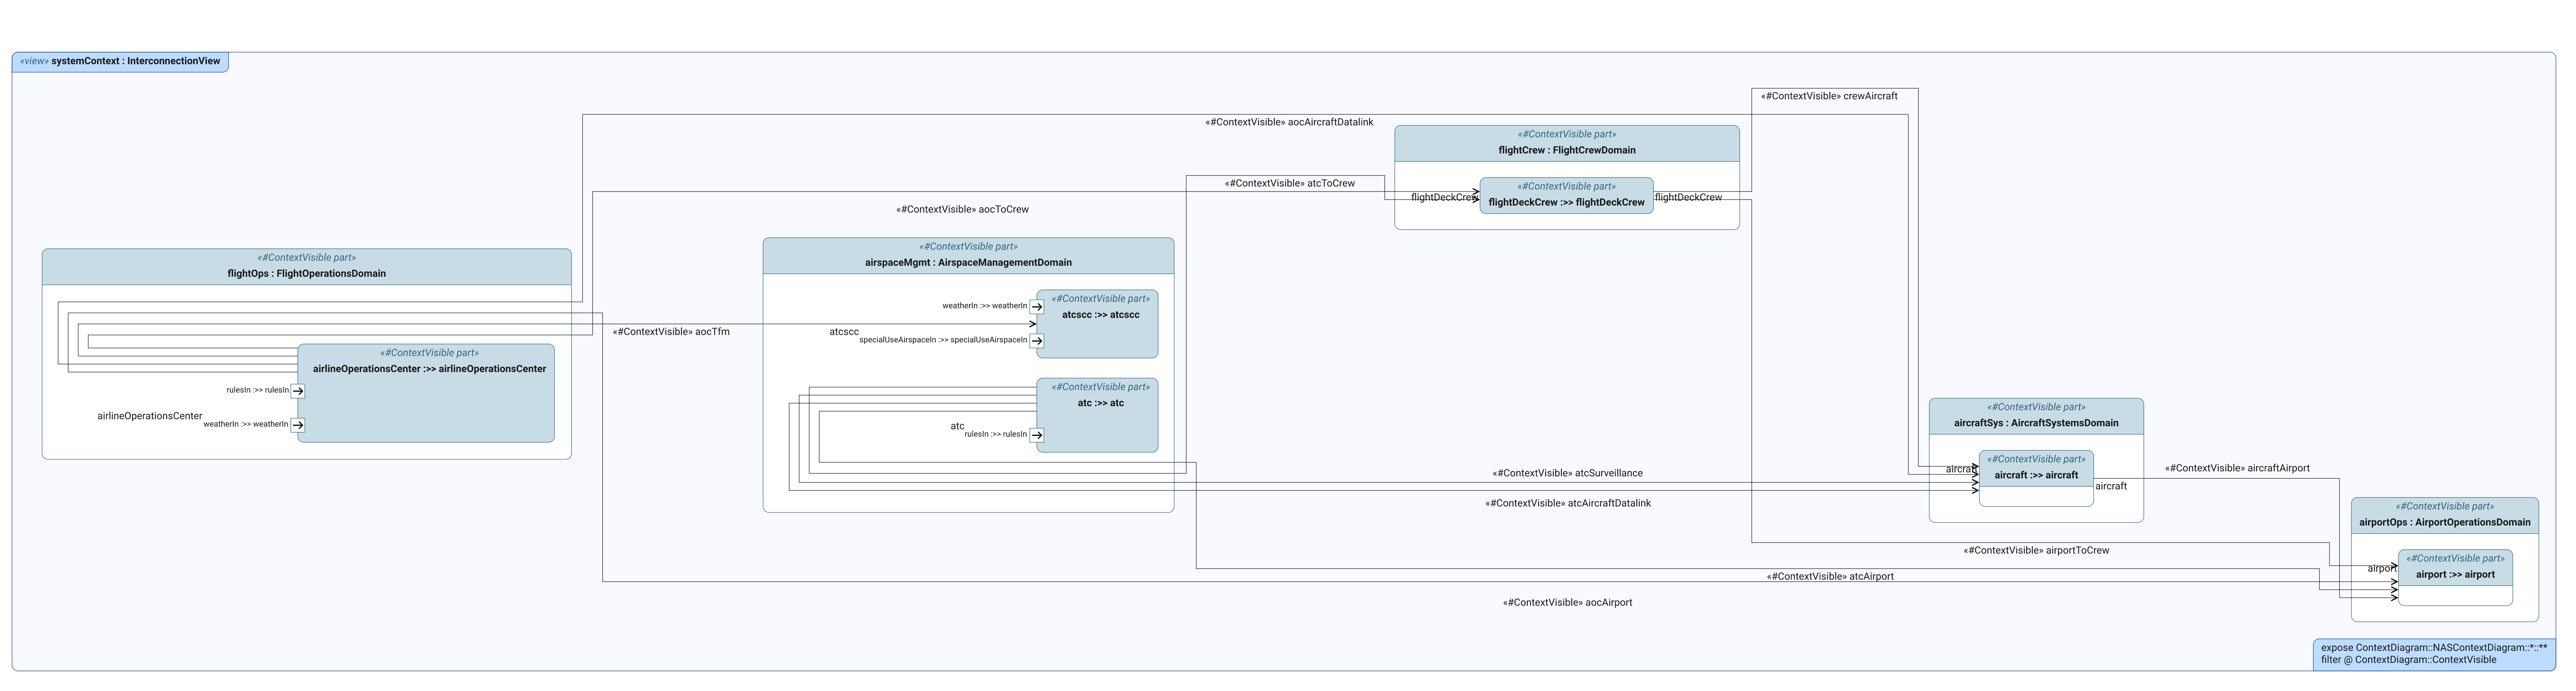
\includegraphics[width=\linewidth,height=0.8\textheight,keepaspectratio]{sysml/diagram-systemContext}
\caption{NAS context diagram. View \texttt{systemContext}; source \texttt{nas\_context\_diagram.sysml}; rendered 2026-10-10.}
\label{fig:sysml-systemContext}
\end{figure}
\end{landscape}


\subsection{Operational Concept}
\label{sec:conops-results}

% Moved 2026-10-17 from Results and Discussion, unchanged.
% Owner's notes, 2026-10-11 print, page 17: "DO"; "Show full detail 1st, then w/
% abstractions & provide rationale."; "The conops doesn't present my specific
% scenario. Need to update w/ the example conflict."
% The AI-DRAFTED call-out that stood here is removed (scribbled over on the
% 2026-10-13 print, page 24). Still true of the third paragraph: FlyEnroute is not
% yet decomposed in the model, so it describes where the conflict will sit, not
% what the diagram shows today.
The operational concept was first written in full detail as a gate-to-gate thread for one nominal commercial flight, from the pilot's point of view. It runs through eleven phases: the airline's schedule, fleet and crew assignment; the pilot's preparation before duty; reporting and the dispatch release; aircraft preflight and initialization of the flight management system; boarding, loading and fueling; clearance, pushback and taxi; takeoff and initial climb; climb; cruise; arrival planning; and descent through to the gate. Each phase records its initial state, the interfaces in use, and the questions it raised. The full thread is in Appendix~\ref{app:conops}.

The model carries an abstraction of that thread. Figure~\ref{fig:sysml-nominalOpsActivity} shows six actions in sequence: plan the flight, prepare for departure, depart, fly en route, arrive, and close out the flight. The eleven phases were reduced to six because the study concerns one decision in cruise. The phases before departure and after arrival fix the conditions that decision inherits (the aircraft's weight, its cost index, its schedule position) and are kept at the level needed to show where those conditions come from. Detail is added only where the studied decision is made.

The example conflict sits inside the fly en route action. Two aircraft in cruise are predicted to cross at the same level at the same time. The sector controller must move one of them, and each choice costs fuel, time and instructions that fall on different parties. The nominal thread treats a trajectory change in cruise as one step; the experiment of Section~\ref{sec:experiment} opens that step and asks what the decider knows when making it.

\plantodo{S5}{Decompose \texttt{FlyEnroute} one level in \texttt{nas\_activity\_diagram-nominal\_ops.sysml} so the conflict-resolution step appears on Figure~\ref{fig:sysml-nominalOpsActivity}, then check the three paragraphs above against the diagram. Put the full activity breakdown in Appendix~\ref{app:conops}.}

% GENERATED by tools/render_sysml_diagrams.py. Do not edit: the next run overwrites it.
% To change a caption, edit the `// caption:` line above the view in the .sysml file.
% To add or remove a figure, add or remove the view in the model.
% To move a figure between the body and the appendix, add or remove a
% `// placement: body` line above the caption line.

\begin{landscape}
\begin{figure}[!htbp]
\centering
\pdfimageresolution=300
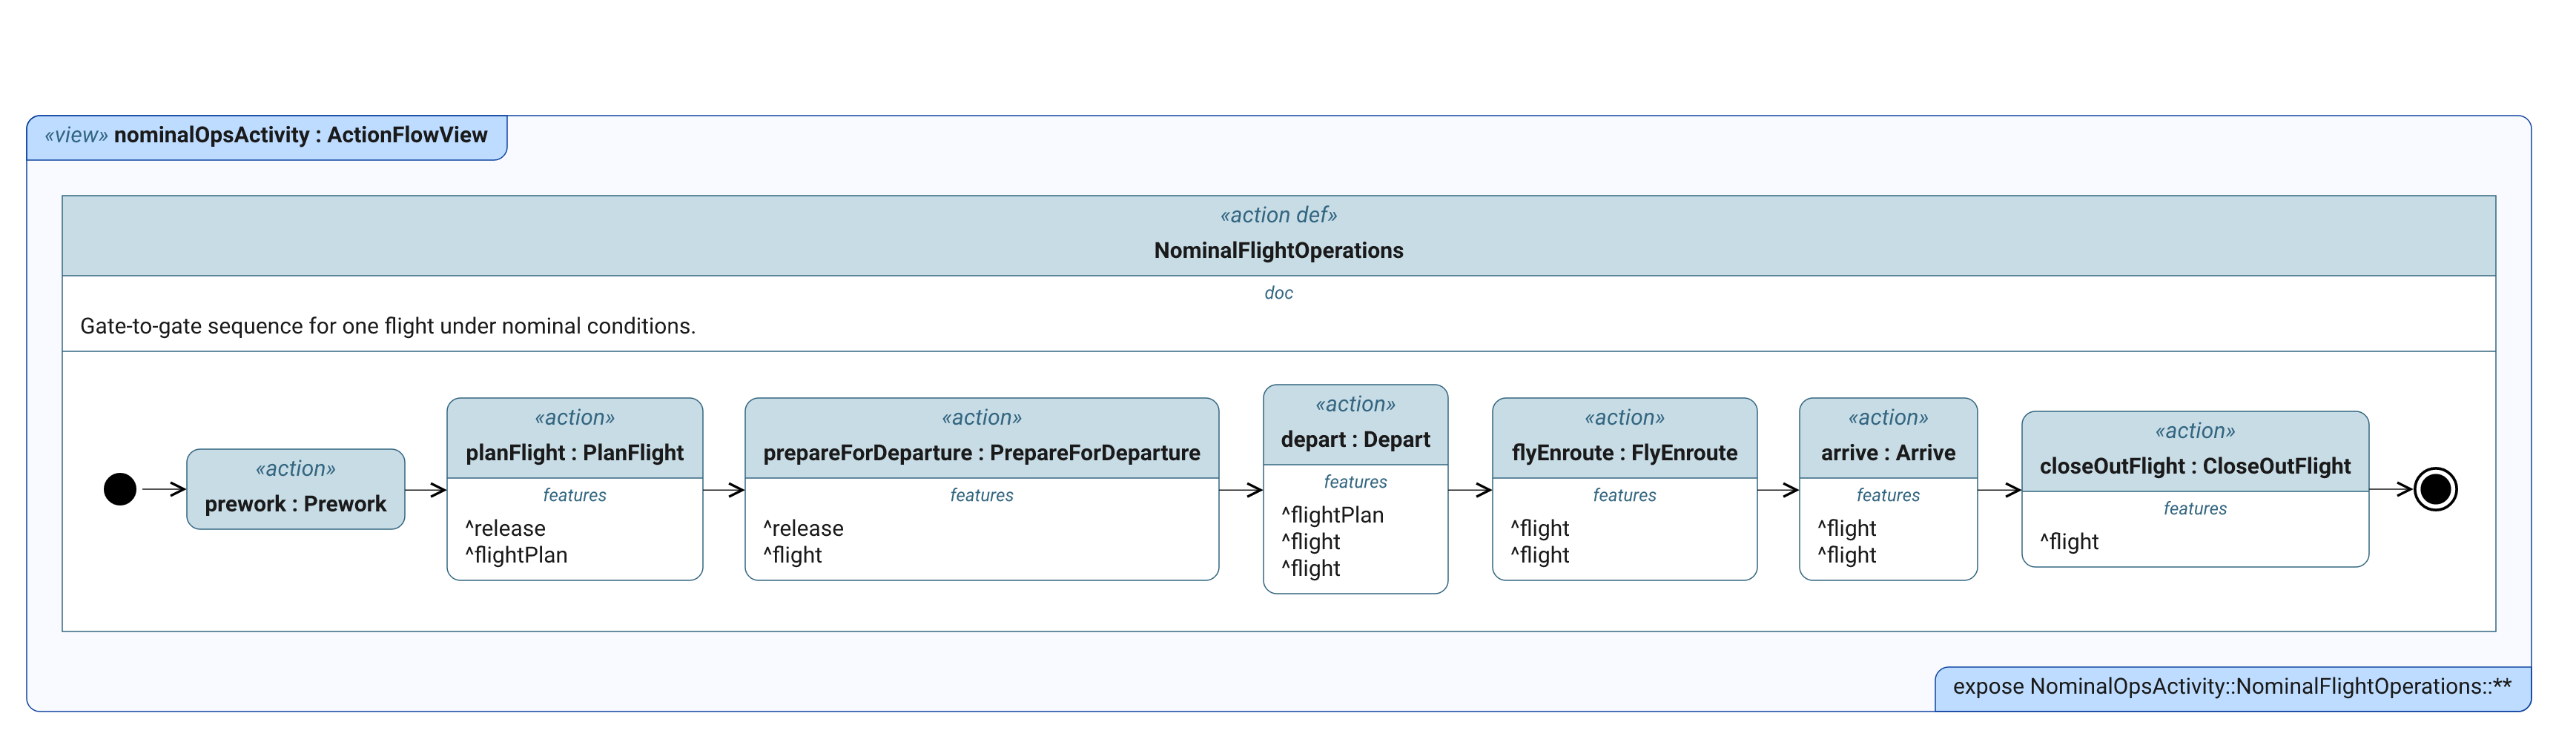
\includegraphics[width=\linewidth,height=0.8\textheight,keepaspectratio]{sysml/diagram-nominalOpsActivity}
\caption{Nominal flight operations activity diagram, phase level (each phase is decomposed in its own figure). View \texttt{nominalOpsActivity}; source \texttt{nas\_activity\_diagram-nominal\_ops.sysml}; rendered 2026-10-18.}
\label{fig:sysml-nominalOpsActivity}
\end{figure}
\end{landscape}


\subsection{Architecture: Detailed and Abstracted}
\label{sec:architecture-results}

% Moved 2026-10-17 from Results and Discussion, unchanged.
% Owner's note, 2026-10-11 print, page 17: "Place detailed & abstracted. Make sub-section."
\plantodo{S10}{Present the SysML architecture: package structure, the context diagram (Figure~\ref{fig:sysml-systemContext}), the internal block diagrams below, the interface and item-flow model, and the requirements model with traceability. For the aircraft, the detailed diagram comes first and the abstracted one second (your note: ``Place detailed and abstracted''); say what the abstraction drops and why. The airspace management diagram is still a placeholder.}

\aidraft{Two connecting sentences so the figures are referred to from the text. Replace with your own description of what each level of detail shows.}
The aircraft is shown at two levels of detail. Figure~\ref{fig:sysml-aircraftIbdDetail} is the detailed internal block diagram, including propulsion, airframe, landing gear, utilities, and the fuel and power links. Figure~\ref{fig:sysml-aircraftIbd} is the abstraction used in the rest of the report: the crew, the flight deck controls, the avionics, the flight controls, the fuel system, and the information and command links among them, which are the parts the studied decision passes through. Figure~\ref{fig:sysml-airspaceManagementIbd} shows the internals of airspace management as modeled so far.
% ---- end AI draft

% GENERATED by tools/render_sysml_diagrams.py. Do not edit: the next run overwrites it.
% To change a caption, edit the `// caption:` line above the view in the .sysml file.
% To add or remove a figure, add or remove the view in the model.
% To move a figure between the body and the appendix, add or remove a
% `// placement: body` line above the caption line.

\begin{landscape}
\begin{figure}[!htbp]
\centering
\pdfimageresolution=300
\includegraphics[width=\linewidth,height=0.8\textheight,keepaspectratio]{sysml/diagram-aircraftIbdDetail}
\caption{Aircraft internal block diagram, detailed level: adds propulsion, airframe, landing gear, utilities, and the fuel and power links. View \texttt{aircraftIbdDetail}; source \texttt{nas\_ibd\_aircraft.sysml}; rendered 2026-10-19.}
\label{fig:sysml-aircraftIbdDetail}
\end{figure}
\end{landscape}

% GENERATED by tools/render_sysml_diagrams.py. Do not edit: the next run overwrites it.
% To change a caption, edit the `// caption:` line above the view in the .sysml file.
% To add or remove a figure, add or remove the view in the model.
% To move a figure between the body and the appendix, add or remove a
% `// placement: body` line above the caption line.

\begin{landscape}
\begin{figure}[!htbp]
\centering
\pdfimageresolution=300

\includegraphics[width=\linewidth,height=0.8\textheight,keepaspectratio]{sysml/diagram-aircraftIbd}
\caption{Aircraft internal block diagram, default level of detail. View \texttt{aircraftIbd}; source \texttt{nas\_ibd\_aircraft.sysml}; rendered 2026-10-19.}
\label{fig:sysml-aircraftIbd}
\end{figure}
\end{landscape}

% GENERATED by tools/render_sysml_diagrams.py. Do not edit: the next run overwrites it.
% To change a caption, edit the `// caption:` line above the view in the .sysml file.
% To add or remove a figure, add or remove the view in the model.
% To move a figure between the body and the appendix, add or remove a
% `// placement: body` line above the caption line.

\begin{landscape}
\begin{figure}[!htbp]
\centering
\pdfimageresolution=300
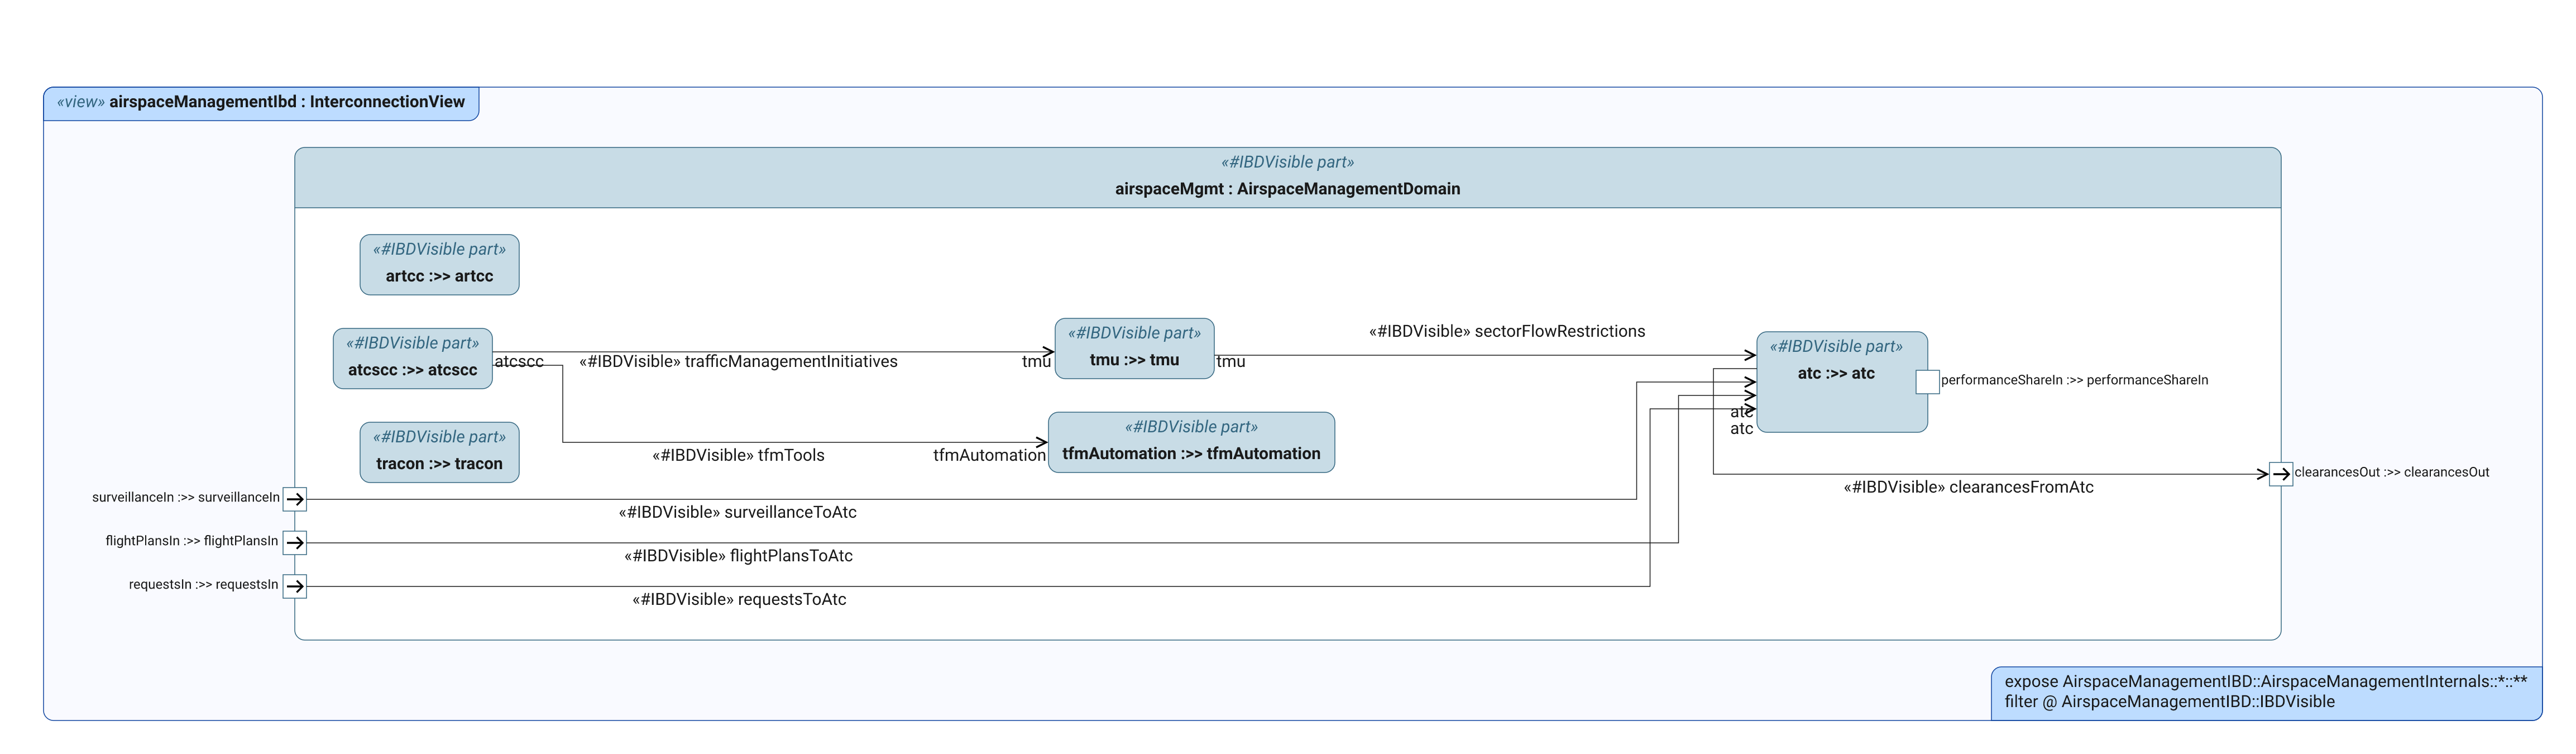
\includegraphics[width=\linewidth,height=0.8\textheight,keepaspectratio]{sysml/diagram-airspaceManagementIbd}
\caption{Airspace management internal block diagram. View \texttt{airspaceManagementIbd}; source \texttt{nas\_ibd\_airspace\_management.sysml}; rendered 2026-10-10.}
\label{fig:sysml-airspaceManagementIbd}
\end{figure}
\end{landscape}


\subsection{Proposed Airline-to-ATC Interface}
\label{sec:proposed-interface}

% Moved 2026-10-17 from Assumptions and Methodology. This answers the owner's
% question on the 2026-10-13 print, page 17 ("This shouldn't be its own section
% here. Where would this fit?"); that call-out is removed. The owner chose this
% place because the subsection leads into the experiment, which explores the
% interface's effect.
\plantodo{Track C (D-019)}{\textbf{Name the digital-thread artifact.} Describe \texttt{AirlinePerformanceShare}: what it carries (gross weight, cost index, connection priority; thrust, drag and fuel-flow model identifiers present but not exercised), who sends it (airline operations center or FMS), who receives it (ATC decision support, per D-012 owned by the system that decides), and which requirements it satisfies (SLR-INF-02) and the goal it serves (SLR-CLR-13). State that security is an assumption. \textbf{Owner's note, 2026-10-11 print: ``important to do''} --- position it against ADS-C EPP and Coppenbarger's Table 2 (the same items, a different receiver); a first draft of that positioning follows.}

% The AI-DRAFTED call-out that stood here is removed (scribbled over on the
% 2026-10-13 print, page 17); the owner's edits to the two paragraphs are applied.
% Still true of the second sentence: the ADS-C EPP statement rests on
% sesarju2019solutionsCatalogue, registered from its title page and contents only.
The items the interface carries are not new. \textcite{coppenbarger1999climbPrediction} listed take-off weight, thrust and drag factors, and the speed profile as candidates for exchange between an airline and air traffic control, and measured what airline-supplied weight does for the prediction of a climb. In Europe, the Extended Projected Profile is sent over ADS-C to downlink the trajectory that the flight management system predicts~\cite{sesarju2019solutionsCatalogue}. What has kept the items out of use is ownership, not feasibility: weight and speed intent ``are considered competitive parameters by airlines and are not available for use''~\cite{schultz2012adaptiveClimb}. A second obstacle is the availability of first-principles data for each aircraft type: thrust, drag and fuel flow.

The proposal here keeps the items and changes the receiver and the purpose. In the earlier work the data feeds a trajectory predictor, to make the prediction of one aircraft's flight path more accurate. Here it feeds the decision support of the party that chooses which aircraft to move, to change the choice. This provides for asking ``what if'' within a mathematical framework. The interface is typed in the model, tagged as part of the improved architecture, and tied to the requirement it satisfies, so the report can point at a model element where the earlier work has a finding in prose. Confidentiality is stated as an assumption: the data is disclosed only to the deciding party, and no security mechanism is modeled.

\aidraft{Closing link to the experiment, written 2026-10-17 (your note: the interface ``provides a good transition to the experiment, which will explore the impact of the new interface''). Replace with your own.}
The experiment that follows measures what this interface is worth. Its cases differ only in what the decider knows: in cases A and B the decider knows only what air traffic control knows today (the aircraft's type, level, speed and route, from which case B assumes a nominal weight), and in cases C and D it also has the items this interface carries. The difference between them is scored against the conflict of Section~\ref{sec:objectives-results}, at the level of the aircraft, the airline, the sector and the system.
% ---- end AI draft

% !TEX root = ../main.tex
\section{Experiment}
\label{sec:experiment}

% Structure of the experiment: knowledge/models/experiment-definition.md and
% knowledge/models/experiment-options-and-scoring.md; decisions D-013 to D-025.

The experiment tests the airline-to-ATC interface proposed in Section~\ref{sec:proposed-interface}, resolving around one conflict with and without the information carried by the proposed interface. Each theoretial resolution is scored at different system boundaries, including those of the aircraft, the airline, the sector and the system.

\subsection{Scenario}
\label{sec:scenario}

The scenario used to explore the value of the proposed interface is a simple one -- four aircraft in one invented en-route sector, shown as one snapshot depicted in Figure~\ref{fig:scenario-plan}: a crossing pair at the same level and two aircraft in trail 2,000 ft below. 

\begin{figure}[htbp]
\centering
\figorbox[0.9\textwidth]{4-ac-scenario_DEN-LAX-crossing.png}{\texttt{attachments/4-ac-scenario\_DEN-LAX-crossing.png}}
\caption{The scenario in plan view. AC1 and AC2 cross at the waypoint at FL380; AC3 and AC4 follow AC1's track at FL360.}
\label{fig:scenario-plan}
\end{figure}

The crossing pair is at FL380, which places the heavy aircraft is near its service ceiling (Figure~\ref{fig:envelope}). The two trailing aircraft are at FL360. The scenario is shown in profile view in Figure~\ref{fig:scenario-profile}. The scenario is static, with no time evolution, similar to the studies that informed the scenario (\cite{kirwan2001coraStrategies}, \cite{fothergill2013resolutionHeuristics}).

\begin{figure}[htbp]
\centering
\figorbox[0.6\textwidth]{4-ac-scenario_altitude_vs_time_plot.png}{\texttt{attachments/4-ac-scenario\_altitude\_vs\_time\_plot.png}}
\caption{Level of each aircraft against its time at the waypoint. AC1 and AC2 arrive together at FL380.}
\label{fig:scenario-profile}
\end{figure}

\plantodo{S11 (owner's note, 2026-10-11 print, page 11)}{\textbf{``Justify one scenario (time) and expand as possible.''} Say that one scenario is studied because of the time available in one term, name what a second scenario would add, and list the variations that are run on the one scenario (similar weights, the climb closed, a crossing pair at or below FL350).}


\subsection{Cases and Resolution Options}
\label{sec:experiment-method}


\plantodo{S11}{\textbf{More realistic comparison?} Consider expanding to include a case that mimics EPP, which enables better understanding of the current trajectories and speed envelope (as evidenced by ETA windows). What else can be derived from EPP info in a split-second assessment? Also, should we throw "typical weight errors" into the tool and see their impact on the system's ability to make good decisions? How might that factor into the model?}

Four cases are considered of varying levels of apriori information, and are summarized in Table~\ref{tab:cases}. The decider's knowledge of the aircraft's perfomance and the relative expense of airline costs determines which resolution options it can offer. 

\begin{table}[h]
\centering
\caption{Conflict resolution options available to a controller with different levels of information about the aircraft. }
\label{tab:cases}
\begin{tabular}{@{}llp{6.2cm}l@{}}
\toprule
Case & Decider & Information & Climb rule applies? \\
\midrule
A & Controller, by rule & Type, level, speed, route & Yes \\
B & Controller, with decision aid & Nominal weight per type & Yes \\
C & Controller, with decision aid & Shared weight and cost index & No \\
D & Controller, with decision aid & Shared weight, cost index and delay margin & No \\
\bottomrule
\end{tabular}
\end{table}

Case A is the baseline, which is the current NAS practice. It has only the information that is currently available to the controller through current interfaces, which limits the options it can offer. \cite{engility2014tasarAlaska} observed that controllers prefer to descend aircraft rather than climb them, and that they will not offer a climb if the aircraft is above FL350. The baseline case applies this rule, which limits the options it can offer. \cite{rantanen2012conflictManeuvers} found that a single descent advisory was the most common resolution option.

Case B is an automated decision aid that has access to the nominal weight of each aircraft type, but not the actual weight or cost index. As such, the system does not have the information needed to guarantee that a climb is feasible. If an unachievable climb is proposed, the flight crew would have the obligation to reject it, leading to unacceptable delays in conflict resolution. As such, the system must also apply the climb rule in Case B. 

Case C is an automated decision aid that has access to the actual weight and cost index of each aircraft. As such, it is not bound by the same limitations as Case B. It differs from  Case D through the ability to account for the cost of delaying the time of arrival of the aircraft. The cost calculation os Case D incorporate a measure of the cost of delaying a flight with connections past its threshold, which is not available to Case C.

\begin{table}[h]
\centering
\caption{Resolution options. A dash means no instruction. Full version with instruction counts in Appendix~\ref{app:optimization}.}
\label{tab:options}
\begin{tabular}{@{}lllll@{}}
\toprule
Option & AC1 & AC2 & AC3 & AC4 \\
\midrule
O1 & Descend 2,000 ft & -- & -- & -- \\
O2 & -- & Descend 2,000 ft & -- & -- \\
O3 & Climb 2,000 ft & -- & -- & -- \\
O4 & -- & Climb 2,000 ft & -- & -- \\
O5 & Turn behind AC2 & -- & -- & -- \\
O6 & -- & Turn behind AC1 & -- & -- \\
O7 & Reduce speed & -- & -- & -- \\
O8 & Descend 4,000 ft & -- & -- & -- \\
O9 & Descend 2,000 ft & -- & Slow or turn & --\\
\bottomrule
\end{tabular}
\end{table}

\plantodo{S11}{\textbf{Resolution options.} State which aircraft descends and the tie-breaker (undecided), and whether the aircraft is cleared back up. For each option give the instructions it costs now, the follow-up it creates, and what the decider must know to use it. Cite \cite{fothergill2013resolutionHeuristics} for the instruction accounting.}

The conflict depicted in the scenario can be resolved by several options, which are listed in Table~\ref{tab:options} and are available to all four cases, with the exception of options 3 and 4, which are not available for cases A and B for reasons described previously.

Options 1 and 2 are descents of the heavy and light aircraft, respectively. A descent is the most common resolution option observed in practice \cite{rantanen2012conflictManeuvers}. It is the safest option, as it is robust to heavy aircraft, which may be operating near their service ceiling with little room to maneuver. Cases A and B will be unable to discern a difference in cost between the two options due to limited knowledge. 

Options 3 and 4 are climbs of the heavy and light aircraft, respectively, which are not available to cases A and B due to the climb rule. If A and B were able to consider climbs they would be similarly ignorant to the relative benefit and safety associated with the lighter aircraft climbing. 

In Options 5 and 6, a lateral modification is assigned by the controller to achieve separation without the need for changes to flight level. Option 7 considers a speed reduction of the heavy aircraft, which is a less common resolution option, but which is practical and straight forward way to achieve separation if there is sufficient separation on either side of the pair. Aircraft 3 and 4 complicate its application to this scenario. 

Option 8 is a 4,000 ft descent of the heavy aircraft, which a controller may deem necessary to simplify the separation with aircraft 3 and 4, which are in trail 2,000 ft below aircraft 1. Option 9 is a descent of the heavy aircraft and a speed reduction or turn of the light aircraft, which is a less common resolution option.

While not comprehensive, this set of options is representative of controller practices. \cite{fothergill2013resolutionHeuristics} found that controllers relied on five lateral vectoring heuristics and eight vertical level-change heuristics to resolve potential conflicts between aircraft. \cite{rantanen2012conflictManeuvers} found that level-offs constituted the most frequent maneuver category, which are only applicable to aircraft ascending or descending and which represented 44\%. Turns were the next most frequent, at 32\%, followed by descents at 18\%, and climbs at 5\%. Turns occurred much less frequently than vertical trajectory changes, accounting for 32\% compared with 68\%. These percentages reflect actions taken across all types of conflicts, rather than the cruise scenario alone. 

\plantodo{S11}{\textbf{To Specify} degree of turn, distance offset, and re-vectoring back on path, whether direct-to or otherwise. This will manifest in different costs.}

\subsection{Scoring}
\label{sec:scoring-method}

Each option is scored along several lines, to highlight the ways different actions lead to different costs and how those costs aggregate at varying system of interest boundaries, including:
\begin{itemize}
    \item a single aircraft,
    \item all aircraft associated with a single airline,
    \item all aircraft in the sector,
    \item the airspace as a whole, including the cost of controller actions, airline schedule impacts, and environmental impacts.
\end{itemize}

\plantodo{S11}{\textbf{Review items.} Still need to be checked against \texttt{simulation/experiment\_scoring.py}. Also, need to finalize what costs will be included where, based on the models. Current content is a draft.}

Individual aircraft costs are limited to time and fuel, and are equated through the use of a standard industry conversion with the cost index (CI). For aircraft $i$ the cost of an option is its extra fuel plus its cost index times its extra time, in kilograms of fuel, the form used in \cite{mori2022massCruise}:
\begin{equation}
c_i = \Delta m_{f,i} + \mathit{CI}_i\, \Delta t_i ,
\label{eq:ac-cost}
\end{equation}
where the extra fuel $\Delta m_{f,i}$ and the extra time $\Delta t_i$ are the option minus the baseline of flying on undisturbed, and $\mathit{CI}_i$ is the cost index of aircraft $i$ in kilograms of fuel per minute.

An airline's cost is the sum over its aircraft plus a step cost when a flight misses a connection, plus CO2 converted to dollars. 

The cost experienced by the sector include all individual aircraft costs as well as clearances issued, effort to devise them, and residual risk. The latter three costs are associated with the sector

Total airspace cost is that of the system of interest, and totals all costs experienced by airspace users and by the stakeholders of the system. As such, it includes the environmental cost associated with each action. This would also consider the balance of costs across airlines, if the scenario facilitated resolutions that lead to inequitable costs. 

\plantodo{S11}{\textbf{Emissions.} State the conversion from fuel to CO2 and its source (\cite{icao2024icecMethodology}). State how CO2 becomes dollars at the airline level and why that route was chosen (credit price, passenger value, or both; undecided), and why the system level keeps CO2 in kg.}


\subsubsection{Case Considerations}


Case A applies its rule, one descent. Each automated case chooses, among the options it is allowed to offer, the option whose estimated total of Eq.~\ref{eq:ac-cost} over all aircraft is lowest. Case B uses the type's nominal mass for every aircraft and values time at 1 kg/min. Cases C and D use each aircraft's actual mass and cost index. Case D also rejects an option that delays a flight with connections past its threshold. Whatever a case chooses is then scored at the actual masses, and that score is what the tables report.

Schedule reliability enters as a step cost, as described by \cite{pilon2019udppMargins}, which occurs when a flight with connections is delayed past a given threshold. At the time threshold associated with missed connections, the flight incurs a cost $K$ on top of Eq.~\ref{eq:ac-cost}. No sourced value of $K$ is presently held, so the tables report whether the threshold is crossed, not a dollar figure. This may change in a future draft. 

Carbon dioxide can be derived from the chemical formula of Jet-A fuel, as 3.16 kg per kilogram of fuel \cite{icao2024icecMethodology}. Instructions issued by controllers are counted for those required to resolve the initial conflict as well as those to clear the aircraft back to its original path, but are not presently converted to a USD cost.

\begin{figure}[htbp]
\centering
\figorbox[0.7\textwidth]{single_flight_cost_per_delay.png}{\texttt{attachments/single\_flight\_cost\_per\_delay.png}}
\caption{Cost of delay for one flight, with steps where a margin is exceeded. Reproduced from \cite{pilon2019udppMargins}, Figure 1.}
\label{fig:cost-of-delay}
\end{figure}

\subsection{Aircraft Model and Its Simplifications}
\label{sec:scoring-limits}
Calculating a fuel and time cost involves defining a truth model to enable comparison of the resultant airspace performance observed as a result of resolving conflicts using the various optoins. The OpenAP (open aircraft performance model, TU Delft) is used to define that entitled information and supplies fuel flow, thrust and drag for the scenario aircraft, which are combined in the equations of motion to determine fuel and time deltas.

Each aircraft is a point mass in steady flight at a constant Mach number. Drag, maximum thrust and fuel flow are taken from OpenAP \cite{sun2020openap}, which uses a two-term drag polar and, above 30,000 ft, the two-shaft turbofan thrust model of \textcite{bartel2008thrustFuel}. 

\plantodo{S11, S12}{\textbf{OpenAP Review}Read Sections 5 and 7 of the OpenAP paper (pp.~6 to 17) before submission. What the paper says about its own accuracy is in \texttt{evidence/literature-notes/summaries/4 - sun2020openap.md} and belongs in the discussion of the truth model's uncertainty (Section~\ref{sec:experiment-results}).}

A descent is flown at 1,500 ft/min. A climb is flown at maximum thrust, at the rate that thrust allows and no more than 1,500 ft/min. A level is available to an aircraft only if it would still have 150 ft/min of climb left there. Cases A and B do not know the mass and so cannot make that test; they offer a climb only at or below FL350, which the scenario does not explore. Cases C and D make it at the aircraft's actual mass. Figure~\ref{fig:envelope} depicts a typical flight envelope, drawn assuming lift equals weight and using the OpenAP models. 

\begin{figure}[htbp]
\centering
\figorbox[\textwidth]{b739_envelope.png}{PLACEHOLDER: run \texttt{simulation/b739\_envelope.py} to produce \texttt{report/figures/b739\_envelope.png}}
\caption{The heavy B737-9 (71.0 t) has little room left to change speed or level at FL380. Left: cruise envelope, with three lines of constant rate of climb left: 0 ft/min (thrust equals drag), 100 ft/min (the service ceiling, \cite{faa2015ac61107b}) and 150 ft/min (the operator margin the scenario uses). Right: width of the usable speed band and rate of climb left at Mach 0.80, by flight level.}
\label{fig:envelope}
\end{figure}

The low-speed boundary is 1.3 times the stall speed at an assumed clean maximum lift coefficient, and its high-speed boundary is the more restrictive of the maximum operating Mach number and the maximum operating speed (VMO). The aircraft's present level and Mach number are marked, and each altitude and speed instruction the scenario offers it is marked as inside or outside the region with 150 ft/min of climb left. Speed changs of +/- 0.04 Mach are presented, as these are typical simplifications employed by European controllers. The weight chosen for the figure shows the limitations associated with the speed simplifications, both in their inability to use the full speed change authority available to the aircraft and to forsee rejections that pilots will invevitably convey upon clearance issuance. 

The model makes the following simplifications.
\begin{enumerate}
\item \textbf{Standard atmosphere, no wind, lift equal to weight.} Time differences come only from true airspeed and added track distance.
\item \textbf{No compressibility drag.} The drag used here has no Mach-number term, though its supported by OpenAP and has a non-trivial impact at Mach numbers above 0.75. 
\item \textbf{The drag polar is the 737 MAX 8's.}
\item \textbf{The fuel curve is the package default.} OpenAP has no fuel model fitted to the 737 MAX 9 or MAX 8; it uses its default coefficients scaled by the LEAP-1B take-off fuel flow.
\item \textbf{The climb margins.} The service ceiling is the level with 100 ft/min of climb left \cite{faa2015ac61107b}. The 150 ft/min the experiment requires is commonly observed in practice.
\item \textbf{One climb rate per climb.} The rate is taken at the mid-altitude and held; the climb is not integrated. A climb is not checked against the time left before the crossing.
\item \textbf{Mass is constant.} Fuel burned during the manoeuvre does not reduce the mass.
\item \textbf{The low-speed limit rests on an assumed maximum lift coefficient} ($C_{L\max} = 1.45$) and is a stall margin, not a buffet boundary.
\end{enumerate}

% !TEX root = ../main.tex
\section{Results and Discussion (Preliminary)}
\label{sec:results}

\irtwo{Results and Discussion (preliminary). For Interim Report \#2 this section needs: (1) the architecture as it stands (context diagram, aircraft IBD, the three requirements tagged \texttt{improved} as the measured gap) --- the figures are now in Section~\ref{sec:system-model}; (2) the two hand checks from \texttt{experiment-definition.md} \S9 written up as preliminary results; (3) the first OpenAP numbers --- Figure~\ref{fig:fuelflow-altitude} and Table~\ref{tab:outcomes} are in place, the discussion is not; (4) one paragraph on what is not yet done.}

\subsection{Model Results}
\plantodo{S10, S13 (D-028)}{\textbf{Model results.} With the architecture now presented in Section~\ref{sec:system-model}, report its measures here, against the measures named in Section~\ref{sec:deliverables}: for example, how many stakeholder requirements trace to a kept objective, how many system requirements are allocated to a constituent system, and which requirements are tagged \texttt{improved} because today's NAS does not meet them. Without this, the systems engineering work is described but never assessed.}

\subsection{Experiment Results}
\label{sec:experiment-results}

% The table body is generated by simulation/experiment_scoring.py (do not edit the
% file it inputs). It replaces the hand-typed table whose cells were empty.
\begin{table}[h]
\centering
\small
\caption{Outcome of each case at four levels, for the base scenario scored at the actual masses. Each cost is a difference from flying on undisturbed. Preliminary: the scenario's numbers are not all confirmed.}
\label{tab:outcomes}
% Generated by simulation/experiment_scoring.py; do not edit. Fidelity: actualMass
% Scenario: base; run 2026-10-29
\begin{tabular}{@{}llp{3.0cm}p{3.2cm}p{2.6cm}p{2.4cm}@{}}
\toprule
Case & Option & Largest cost to any one aircraft (kg fuel-equiv.) & Airline totals (USD) & Sector (calls / effort / risk) & System fuel, CO2 (kg) \\
\midrule
A & O10 & 40 (AC2) & X 0, Y 102, Z 0 & 1+1 / 1 / low & 41, 130 \\
B & O8 & 26 (AC1) & X 66, Y 0, Z 0 & 1+1 / 3 / low & 32, 102 \\
C & O4 & 12 (AC2) & X 0, Y 32, Z 0 & 1+1 / 3 / low & 12, 39 \\
D & O4 & 12 (AC2) & X 0, Y 32, Z 0 & 1+1 / 3 / low & 12, 39 \\
\bottomrule
\end{tabular}

\end{table}

\plantodo{S12}{\textbf{Which option each case chose, and why.} Walk Table~\ref{tab:outcomes} row by row. For case A, name the rule that produced the choice. For B, C and D, name the cost that decided it.}

\plantodo{S12}{\textbf{Did the climb rule matter?} With the crossing pair above FL350, cases A and B could not offer a climb and cases C and D could. Say whether case C used one, for which aircraft, and what it saved. If C did not climb either, say so: that is a result too.}

\plantodo{S12}{\textbf{B minus A, and C minus B.} The first is what automation is worth; the second is what the information exchange is worth. Compare the size of each with the prior figure of tens of gallons per flight (\cite{engility2014tasarAlaska}, p.~12) and say whether the difference is larger than the truth model's uncertainty.}

\plantodo{S9, S12}{\textbf{Does the best option change with the level?} Read across each row of Table~\ref{tab:outcomes}. Name any option that is better for one aircraft or one airline and worse for the sector or the system, and who pays (the largest cost to any one aircraft). This is the sub-system versus system discussion.}

\plantodo{S12}{\textbf{Airline X's two flights.} Discuss the option that touches both of one airline's aircraft: what the airline would choose between its late flight and its early one, and that the controller cannot see that preference. Connect to the dispatcher priorities (schedule integrity and connections rated at or above fuel; source of that table still to confirm).}

\plantodo{S12}{\textbf{Workload is three things.} Discuss clearances issued, effort to devise, and residual risk separately. Say where a ``more workload'' option on one of them is ``less'' on another.}

\plantodo{S12}{\textbf{When would the controller say no?} (owner's note, second hand review, 5.2). Discuss whether refusals are more likely in morning rushes at hub airports or near holidays, using the sector-loading rule in \cite{engility2014tasarAlaska} (p.~10). A hypothesis; needs a source.}

\plantodo{S12}{\textbf{Is schedule the right priority?} (owner's note, second hand review, 4.11). Contrast a carbon price, which makes fuel weigh more against time, with controllers' usual practice of giving schedule the priority.}

\begin{figure}[h]
\centering
\figorbox{b739_fuelflow_altitude.png}{PLACEHOLDER: run \texttt{simulation/b739\_envelope.py} to produce \texttt{report/figures/b739\_fuelflow\_altitude.png}}
\caption{Fuel flow and specific range against altitude at Mach 0.80 for the heavy and light B737-9 (OpenAP).}
\label{fig:fuelflow-altitude}
\end{figure}

\plantodo{Track A}{\textbf{Figure slot: sequence diagram} of case C's conflict resolution (controller, ATC decision support, airline operations center, FMS, crew), rendered from the model once drafted (turn 3).}

\plantodo{S12}{\textbf{The case where nothing changes.} Report the variation with similar weights and the climb closed, where case C picks the same option as case B, to show the comparison is not rigged.}

Each column of Table~\ref{tab:outcomes} belongs to a part of the context diagram (Figure~\ref{fig:sysml-systemContext}). The aircraft column belongs to the aircraft and its flight crew. The airline column belongs to the airline operations center within flight operations. The sector column belongs to air traffic control within airspace management. The system column belongs to no single part. It is a property of the NAS as a whole, which is the reason no constituent system computes it today and the reason the model is needed to state it.

The exchange that cases C and D add is one interface in the model: the airline operations center's performance share to air traffic control's decision support, carrying gross weight, cost index and the flight's delay margin. It satisfies system requirement SLR-INF-02, which is tagged as part of the improved architecture because today's NAS does not meet it. The interface is not drawn on Figure~\ref{fig:sysml-systemContext}, which shows the baseline.


\subsection{Emissions and Who Pays}
\label{sec:emissions-impact}

\plantodo{S9, S12}{\textbf{Airline level: put CO2 into dollars.} Take the fuel difference between cases from Table~\ref{tab:outcomes}, convert to kg of CO2, then to dollars. State the route used and its source. Candidates: (1) the price of a carbon credit or allowance, if a scheme applies to the flight; (2) passenger value, meaning revenue gained or lost because some passengers choose the flight listed with lower emissions. Make the point that fuel is already counted once as fuel cost and that pricing its CO2 counts the same kilograms again, on purpose.}

\plantodo{S9, S12}{\textbf{Passenger value.} Discuss how passengers see a flight's emissions when booking, and whether that reaches the airline as demand. The author's own practice of choosing lower-emission listings is the motivation, not the evidence: cite a study. Note the gap between one decision in one sector and the label a passenger saw at booking; the link is the airline's average over many flights.}

\plantodo{S12}{\textbf{Scale it honestly.} One conflict in one sector is a small number. If a per-year or fleet-wide figure is offered, state the multiplier and its source (for example, how often level crossing conflicts occur), and label it illustrative.}

\plantodo{S9}{\textbf{Who pays.} For the option the system prefers, name the aircraft or airline that is worse off and by how much. This is the equity discussion.}

% !TEX root = ../main.tex
\section{Impact/Financial Benefits}
\label{sec:impact}

% Revised 2026-10-11 from the owner's hand review of the printed report
% (handwritten/2026-10-11_main.md, notes 20.x and 21.x): two sentences struck from
% the scope flag; the emissions subsection moved to Section "Emissions and Who
% Pays" in 06_results_discussion.tex.

\plantodo{S9, S12 (S16 bullet added this session)}{Quantify the impact of the reference architecture and its experiment. Translate the conflict analysis and the experiment's results into concrete operational terms wherever possible (e.g., delay-minutes, fuel burn, CO2, instructions issued) and into US-dollar terms where a credible conversion exists (e.g., published cost-per-delay-minute figures from the literature review, Section~\ref{sec:litreview}). Also discuss the ethical context and any unintended consequences of the recommendations (equity-minded engineering: whose costs get externalized, and onto whom -- this connects directly to the objectives whose costs are externalized onto another stakeholder, Section~\ref{sec:objectives-results}, and to Section~\ref{sec:emissions-impact}).}

\textbf{Scope flag:} the 503 template expects a quantified financial-benefit statement (the template's sample statements are dollar-savings claims from industry DMAIC-style projects). This capstone is an architecture/SoS project, not a cost-reduction project with a ``before'' baseline in dollars, so a literal dollar-savings figure may not be available or meaningful. Recommend framing impact primarily in operational/systems terms (delay, fuel, emissions, predictability, tradeoff-surface shape) with a dollar estimate offered as an illustrative, clearly-caveated secondary figure rather than the headline metric.

% !TEX root = ../main.tex
\section{Conclusions and Recommendations}
\label{sec:conclusions}
\label{sec:recommendations}

% Merged 2026-10-11 with the former Recommendations section per the owner's note
% on the printed report, page 19: "Combine w/ Conclusions."
% (handwritten/2026-10-11_main.md). 05_recommendations.tex is removed; its
% call-out is the second one below, with the phrase the owner struck taken out.

\plantodo{S15, S16}{Briefly restate the problem, approach, and findings, including potential benefits in relative terms if absolute figures are sensitive or incomplete (e.g., ``reduces network-level delay propagation by an illustrative X\% under the demonstrated scenario'' rather than an unsupported absolute claim). Cover: known architecture omissions, limitations of the selected decomposition (S6), limitations of the experiment (Sections~\ref{sec:assumptions} and~\ref{sec:scoring-limits}), and opportunities for future expansion (e.g., additional off-nominal scenarios, unexplored S9 conflicts, deeper crew/maintenance-routing integration).}

\plantodo{S14, S15}{\textbf{Recommendations.} Restate the main findings from Section~\ref{sec:results} and provide recommendations for moving forward. Include the alternatives considered (alternative stakeholder-weighting schemes from S11) and the criteria used to select the recommended approach. Suggest additional areas of study (candidate: architecture extensions, additional off-nominal scenarios from S15, unexplored myopic-optimization conflicts from S9's catalog).}


% No section body yet contains \cite{} (still plantodo placeholders), so
% \nocite{*} forces the full evidence/sources/references.bib register to
% print now; remove it once the literature-review sections cite sources
% inline and the list should instead reflect only what's actually cited.
\nocite{*}
\printbibliography[title={References}]

% !TEX root = ../main.tex
\newpage
\appendix
\section{Appendices}
\label{sec:appendices}

\plantodo{S5, S7, S10, S11 (general)}{Use appendices for material too
extensive for the main body or of interest to only some readers. Label each
lettered (Appendix A, B, ...), and ensure every appendix is referenced from
somewhere in the main body.}

\subsection{Full Nominal-Flight ConOps}
\label{app:conops}
\plantodo{S5}{Full strategic-planning through postflight/continuation
activity breakdown (see main-body summary, Section~\ref{sec:conops-results}).
The phase activity diagrams are placed below (Fly Enroute is in the body,
Figure~\ref{fig:sysml-flyEnrouteActivity}); add the text that introduces them
and cite each one from it.}

% GENERATED by tools/render_sysml_diagrams.py. Do not edit: the next run overwrites it.
% To change a caption, edit the `// caption:` line above the view in the .sysml file.
% To add or remove a figure, add or remove the view in the model.
% To move a figure between the body and the appendix, add or remove a
% `// placement: body` line above the caption line.

\begin{landscape}
\begin{figure}[!htbp]
\centering
\pdfimageresolution=300
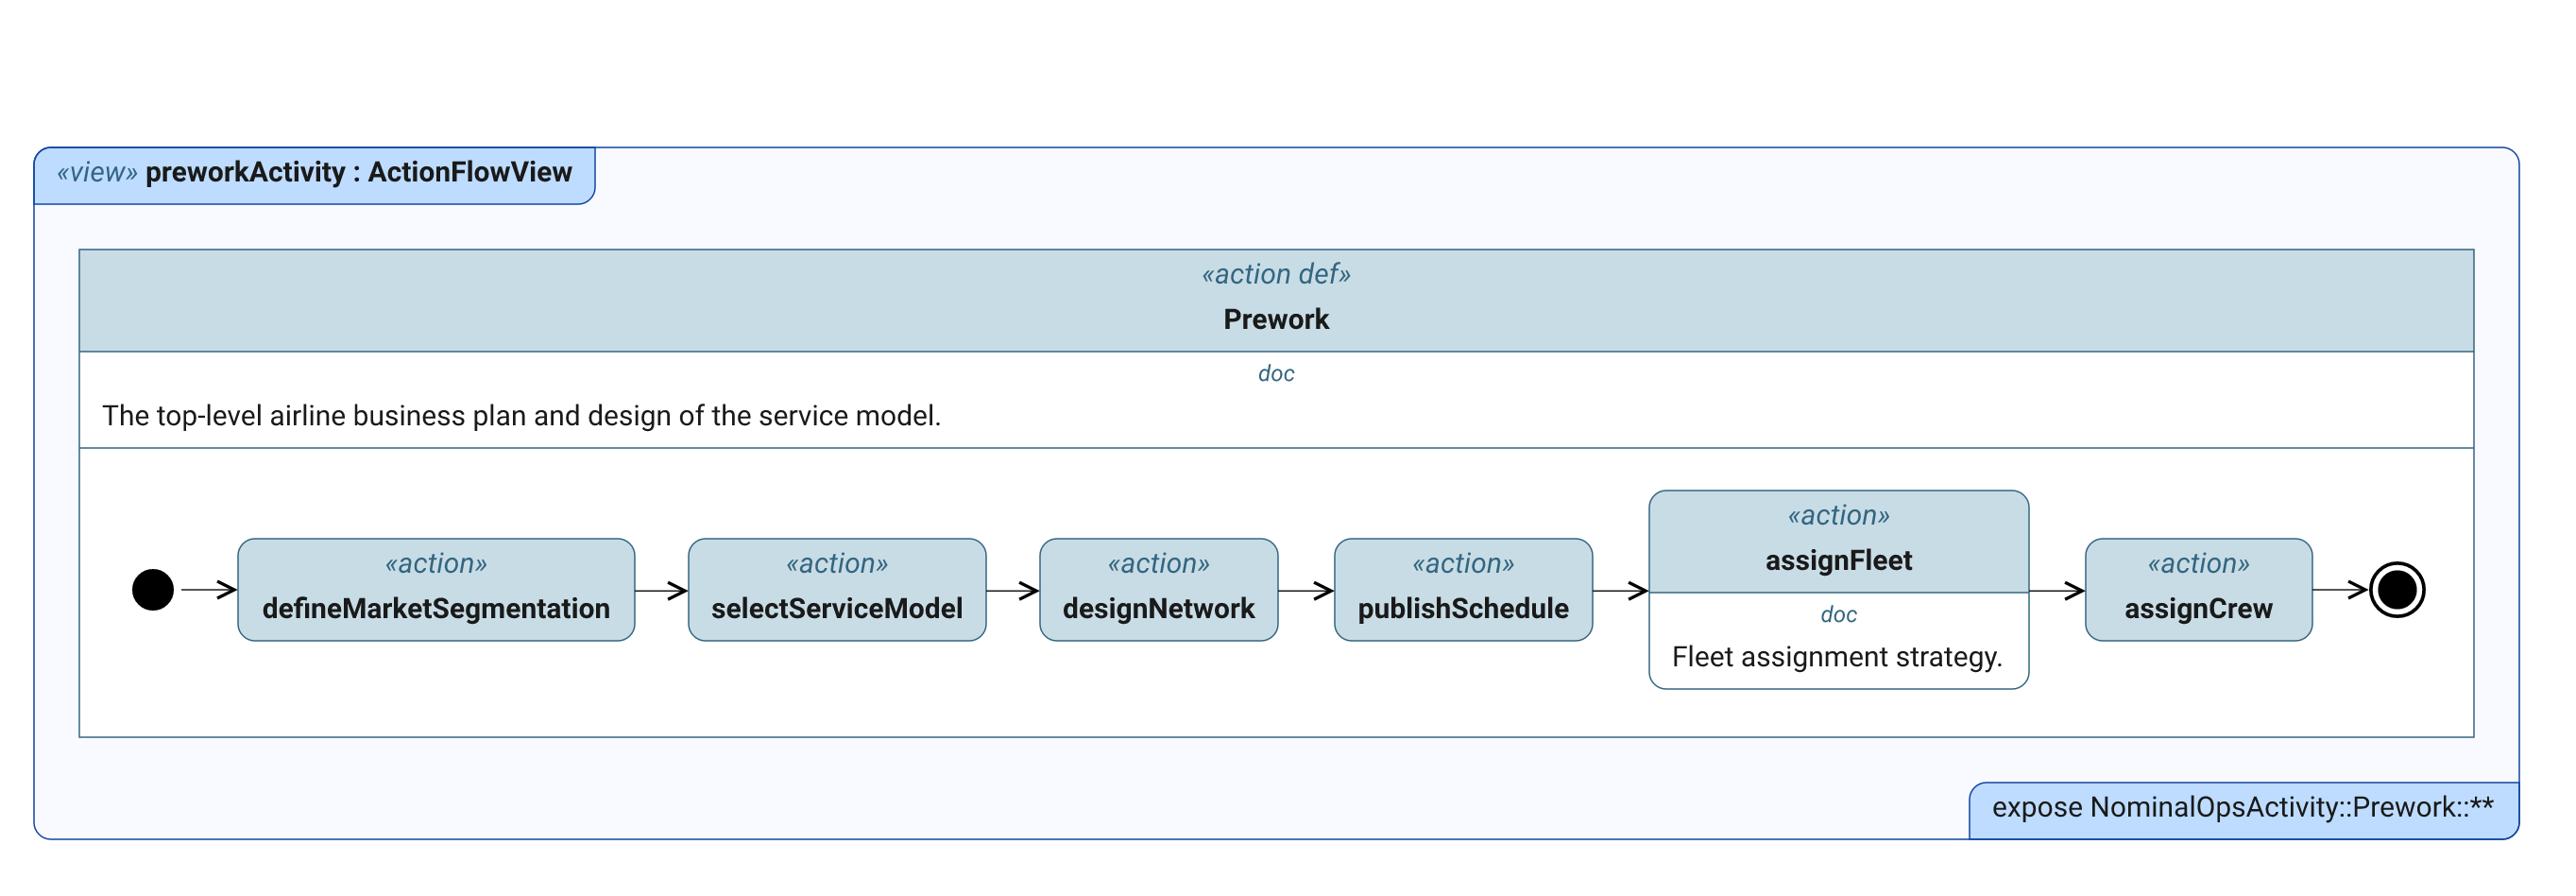
\includegraphics[width=\linewidth,height=0.8\textheight,keepaspectratio]{sysml/diagram-preworkActivity}
\caption{Nominal operations, Prework: airline planning before flight planning. View \texttt{preworkActivity}; source \texttt{nas\_activity\_diagram-nominal\_ops.sysml}; rendered 2026-10-18.}
\label{fig:sysml-preworkActivity}
\end{figure}
\end{landscape}

% GENERATED by tools/render_sysml_diagrams.py. Do not edit: the next run overwrites it.
% To change a caption, edit the `// caption:` line above the view in the .sysml file.
% To add or remove a figure, add or remove the view in the model.
% To move a figure between the body and the appendix, add or remove a
% `// placement: body` line above the caption line.

\begin{landscape}
\begin{figure}[!htbp]
\centering
\pdfimageresolution=300
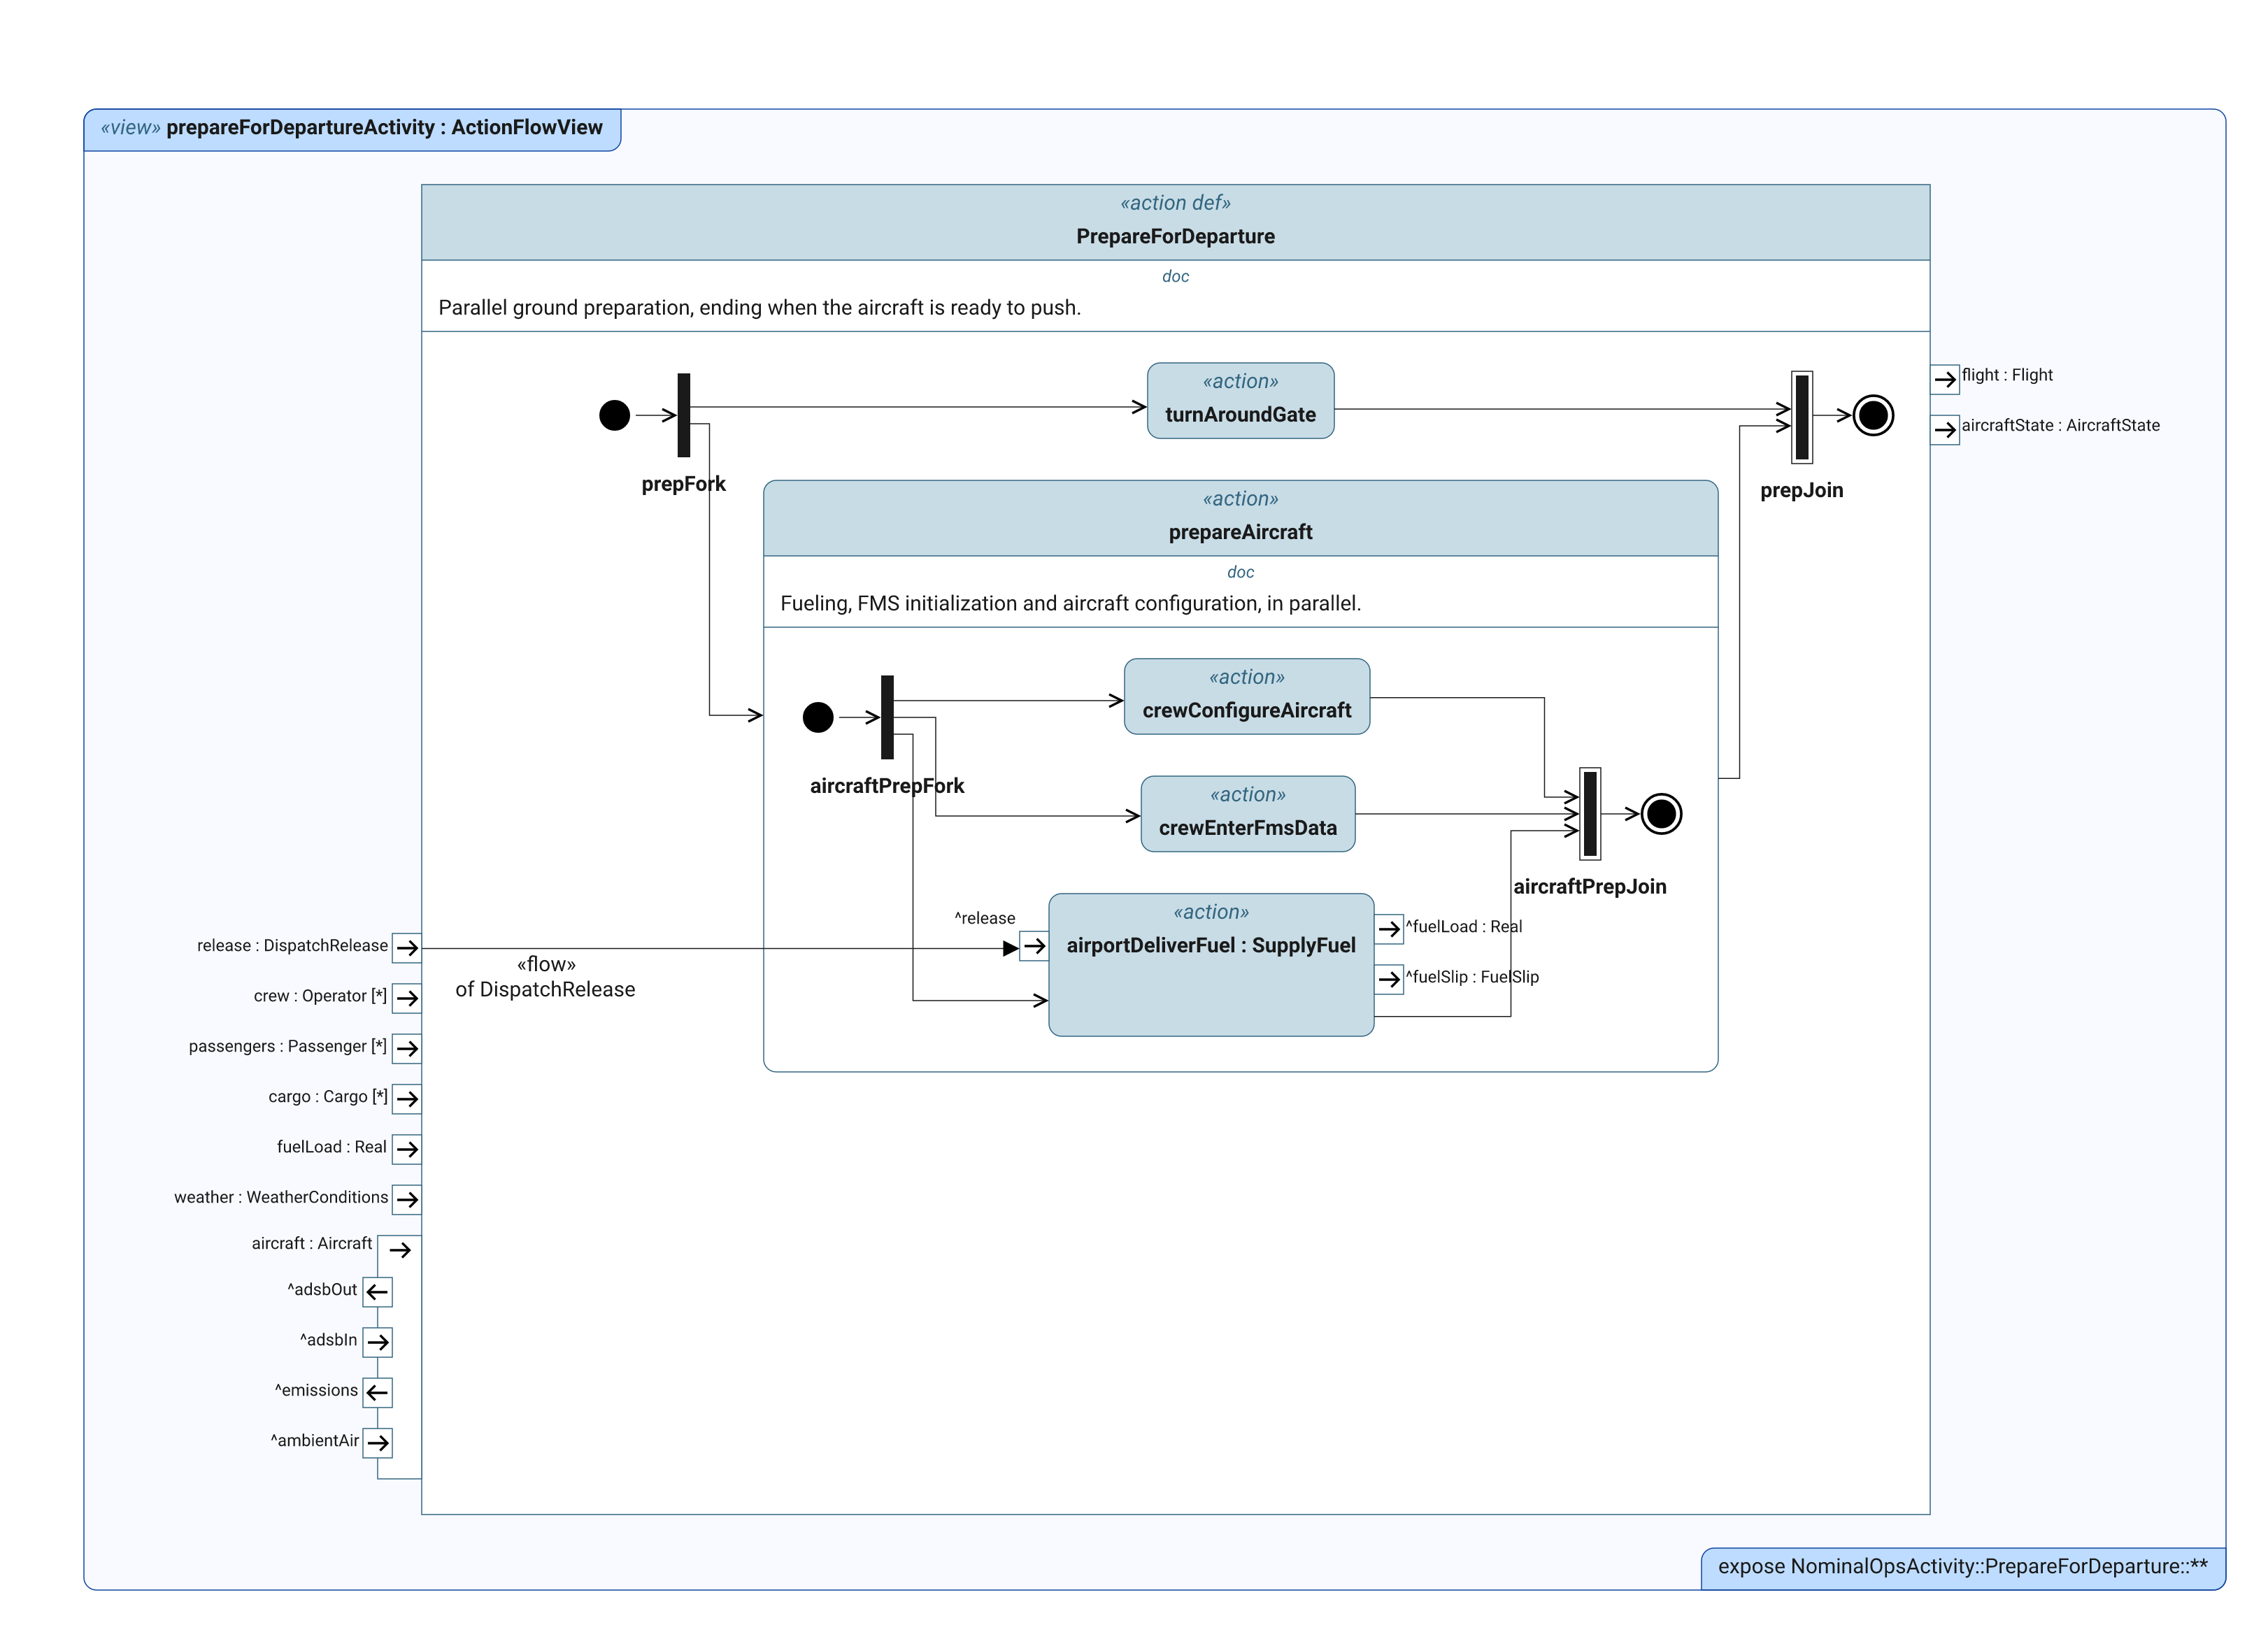
\includegraphics[width=\linewidth,height=0.8\textheight,keepaspectratio]{sysml/diagram-prepareForDepartureActivity}
\caption{Nominal operations, Prepare for Departure: parallel fueling, FMS entry, configuration and gate turnaround. View \texttt{prepareForDepartureActivity}; source \texttt{nas\_activity\_diagram-nominal\_ops.sysml}; rendered 2026-10-19.}
\label{fig:sysml-prepareForDepartureActivity}
\end{figure}
\end{landscape}

% GENERATED by tools/render_sysml_diagrams.py. Do not edit: the next run overwrites it.
% To change a caption, edit the `// caption:` line above the view in the .sysml file.
% To add or remove a figure, add or remove the view in the model.
% To move a figure between the body and the appendix, add or remove a
% `// placement: body` line above the caption line.

\begin{landscape}
\begin{figure}[!htbp]
\centering
\pdfimageresolution=300

\includegraphics[width=\linewidth,height=0.8\textheight,keepaspectratio]{sysml/diagram-departActivity}
\caption{Nominal operations, Depart: clearance, pushback, taxi-out, takeoff and climb. View \texttt{departActivity}; source \texttt{nas\_activity\_diagram-nominal\_ops.sysml}; rendered 2026-10-18.}
\label{fig:sysml-departActivity}
\end{figure}
\end{landscape}

% GENERATED by tools/render_sysml_diagrams.py. Do not edit: the next run overwrites it.
% To change a caption, edit the `// caption:` line above the view in the .sysml file.
% To add or remove a figure, add or remove the view in the model.
% To move a figure between the body and the appendix, add or remove a
% `// placement: body` line above the caption line.

\begin{landscape}
\begin{figure}[!htbp]
\centering
\pdfimageresolution=300

\includegraphics[width=\linewidth,height=0.8\textheight,keepaspectratio]{sysml/diagram-arriveActivity}
\caption{Nominal operations, Arrive: arrival planning, descent, approach, landing and taxi-in. View \texttt{arriveActivity}; source \texttt{nas\_activity\_diagram-nominal\_ops.sysml}; rendered 2026-10-18.}
\label{fig:sysml-arriveActivity}
\end{figure}
\end{landscape}

% GENERATED by tools/render_sysml_diagrams.py. Do not edit: the next run overwrites it.
% To change a caption, edit the `// caption:` line above the view in the .sysml file.
% To add or remove a figure, add or remove the view in the model.
% To move a figure between the body and the appendix, add or remove a
% `// placement: body` line above the caption line.

\begin{landscape}
\begin{figure}[!htbp]
\centering
\pdfimageresolution=300
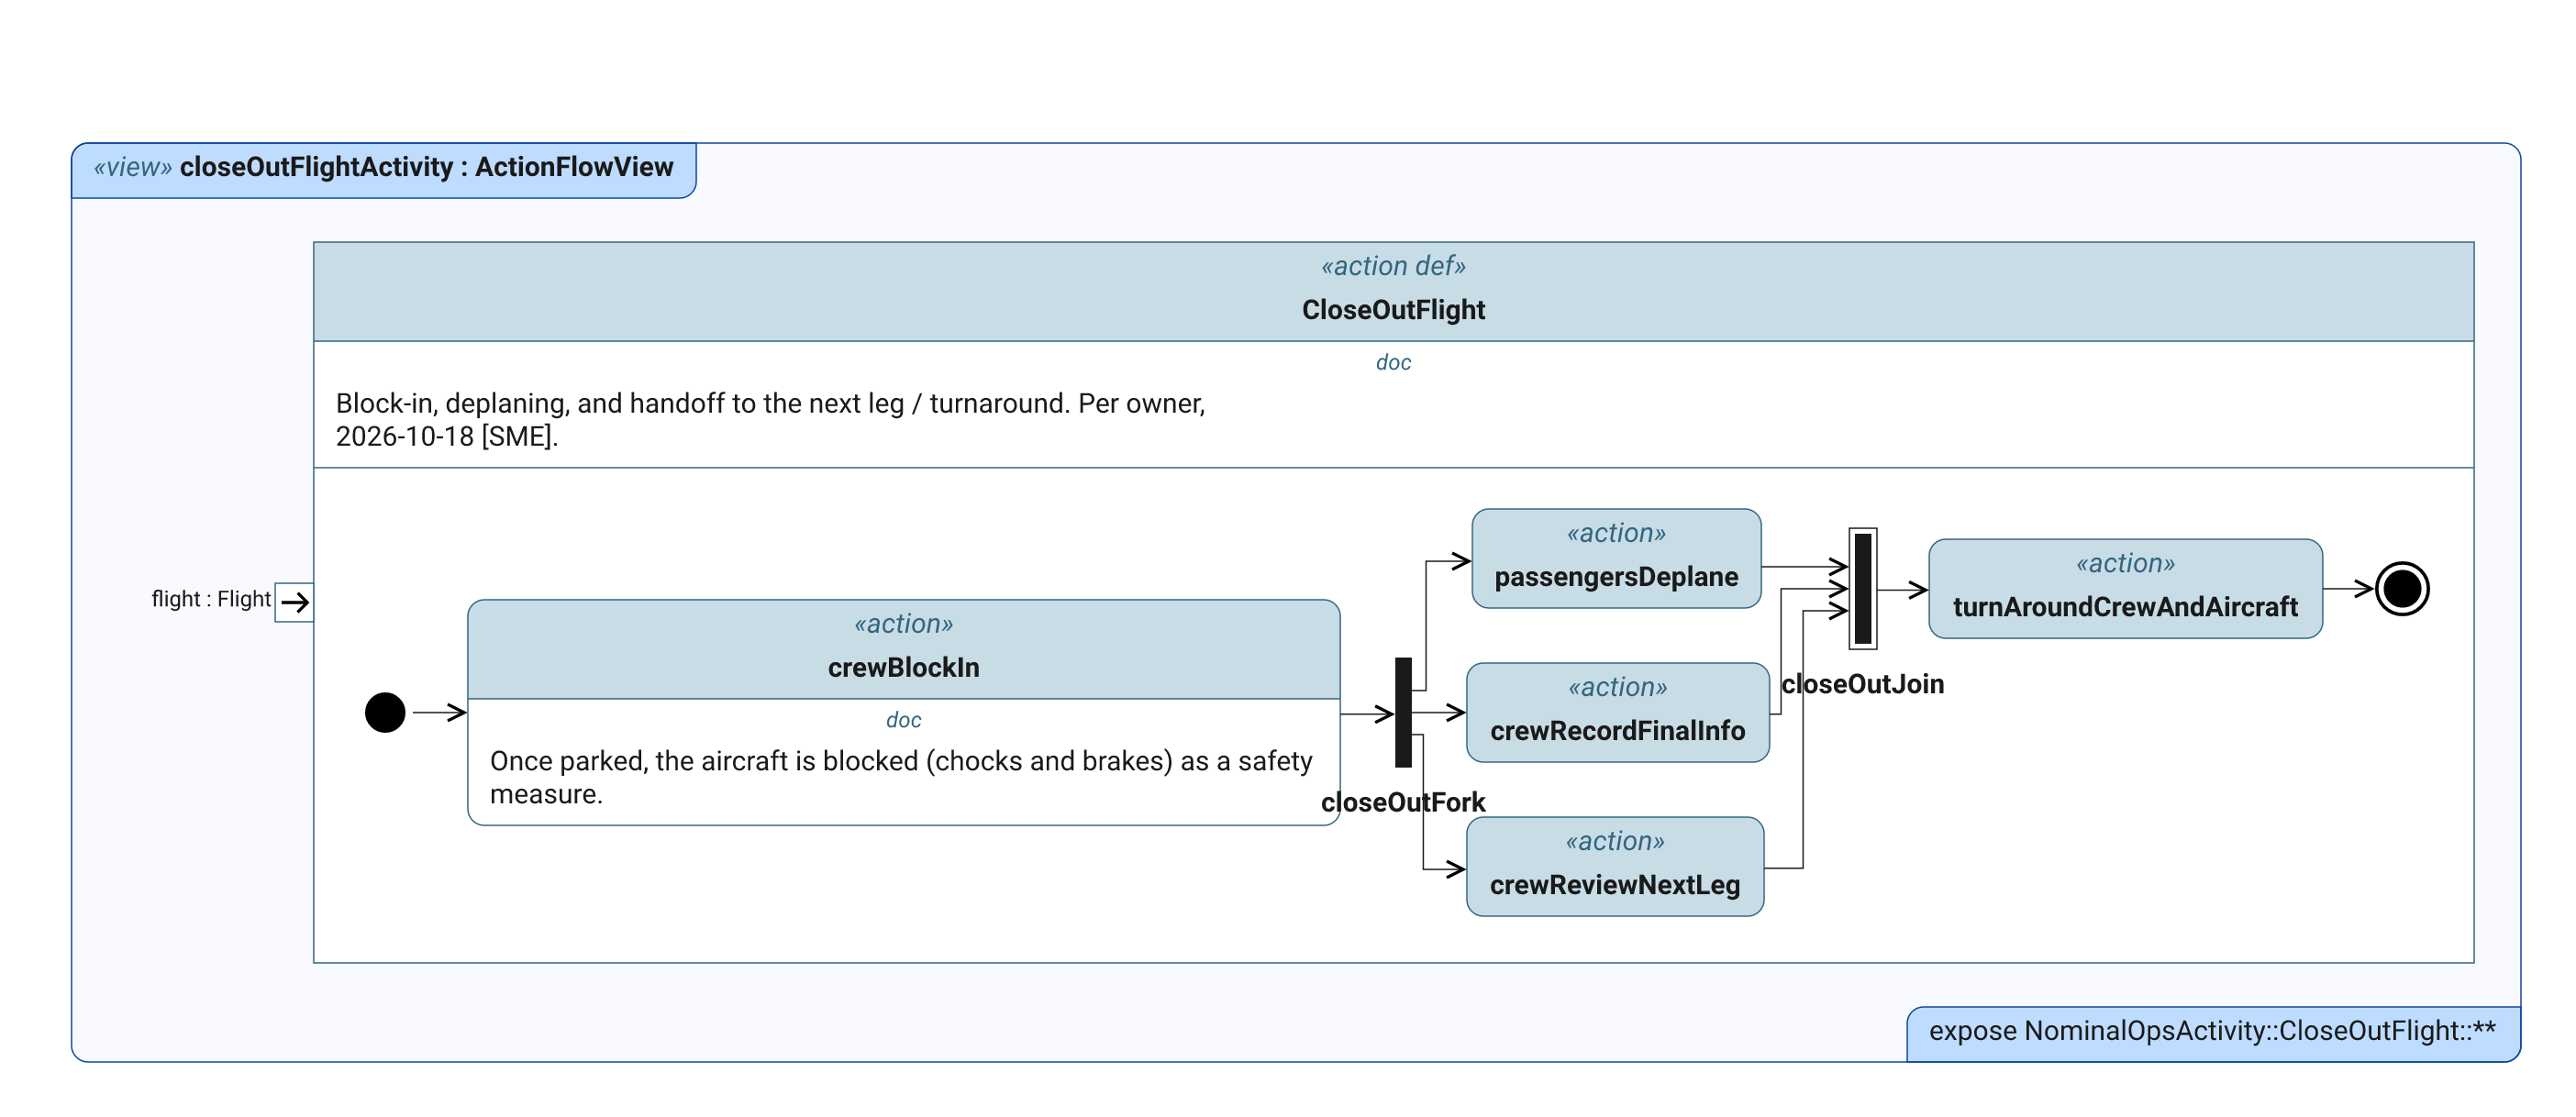
\includegraphics[width=\linewidth,height=0.8\textheight,keepaspectratio]{sysml/diagram-closeOutFlightActivity}
\caption{Nominal operations, Close Out Flight: block-in, deplaning and turnaround. View \texttt{closeOutFlightActivity}; source \texttt{nas\_activity\_diagram-nominal\_ops.sysml}; rendered 2026-10-18.}
\label{fig:sysml-closeOutFlightActivity}
\end{figure}
\end{landscape}


\subsection{Full Stakeholder Register}
\label{app:stakeholders}
\plantodo{S7}{Introduce the two tables below and cite each from the body: the stakeholder assessment (Table~\ref{tab:stakeholder-assessment-excerpt}) and the trace from each stakeholder objective to the requirements (Table~\ref{tab:requirements-objectives}).}

% ---- Generated tables (tools/export_report_tables.py). Do not edit the .tex files in
% figures/tables/: change the stakeholder workbook or the model and rerun the script.
% Owner, 2026-10-22: the whole assessment sheet and the whole objectives sheet go here.
% Generated by tools/export_report_tables.py on 2026-10-22 from knowledge/models/capstone_stakeholder_assessment.xlsx, sheet "Stakeholder Assessment".
% Do not edit: change the source and rerun the script.

\begingroup\footnotesize\setlength{\tabcolsep}{3pt}\setlength{\LTcapwidth}{\textwidth}
\begin{longtable}{@{}>{\raggedright\arraybackslash}p{1.9cm}>{\raggedright\arraybackslash}p{3.3cm}>{\raggedright\arraybackslash}p{3.2cm}>{\raggedright\arraybackslash}p{1.6cm}>{\raggedright\arraybackslash}p{1.6cm}>{\raggedright\arraybackslash}p{0.8cm}>{\raggedright\arraybackslash}p{2.3cm}@{}}
\caption{Stakeholder assessment: all 48 candidate stakeholders, sorted by decision score (\texttt{capstone\_stakeholder\_assessment.xlsx}). Score is standalone importance (high 3, medium 2, low 1) plus trajectory-decision impact (yes 2, indirect 1, no 0); the workbook's other columns (MOPs, MOEs, rationale) are not shown.}\label{tab:stakeholder-assessment-excerpt}\\
\toprule
\textbf{PESTLE domain} & \textbf{Stakeholder} & \textbf{Stated interest} & \textbf{Trajectory impact} & \textbf{Importance} & \textbf{Score} & \textbf{Recommended treatment} \\
\midrule
\endfirsthead
\multicolumn{7}{@{}l}{\textit{Table \thetable{} continued}}\\
\toprule
\textbf{PESTLE domain} & \textbf{Stakeholder} & \textbf{Stated interest} & \textbf{Trajectory impact} & \textbf{Importance} & \textbf{Score} & \textbf{Recommended treatment} \\
\midrule
\endhead
\bottomrule
\endlastfoot
Economic & Adjacent Airspace Users & Throughput and reliability & Yes & High & 5 & Standalone \\
Technical & Air traffic controllers & Predictable aircraft behavior & Yes & High & 5 & Standalone \\
Economic & Airlines & Profitability & Yes & High & 5 & Standalone \\
Economic & Airports & Revenue and capacity & Yes & High & 5 & Standalone \\
Economic & Cargo operators & Throughput and reliability & Yes & High & 5 & Standalone \\
Technical & Dispatchers & Operational optimization & Yes & High & 5 & Standalone \\
Political & Militaries & Navigable airspace \& resources with priority & Yes & High & 5 & Standalone \\
Economic & Engine manufacturers & Product performance and aftermarket revenue & Indirect & High & 4 & Consider /\allowbreak{} Consolidate \\
Social & Flight crews & Workload and quality of life & Indirect & High & 4 & Consider /\allowbreak{} Consolidate \\
Social & Local communities & Noise and environmental impacts & Indirect & High & 4 & Consider /\allowbreak{} Consolidate \\
Environmental & Local communities & Reduced noise & Indirect & High & 4 & Consider /\allowbreak{} Consolidate \\
Social & Business travelers & Schedule reliability & Indirect & Medium & 3 & Consider /\allowbreak{} Consolidate \\
Environmental & Environmental advocacy groups & Reduced emissions & Indirect & Medium & 3 & Consider /\allowbreak{} Consolidate \\
Political & Federal Aviation Administration & Safe and efficient airspace & No & High & 3 & Consider /\allowbreak{} Consolidate \\
Political & ICAO & International standards & Indirect & Medium & 3 & Consider /\allowbreak{} Consolidate \\
Economic & Labor unions & Compensation and job security & Indirect & Medium & 3 & Consider /\allowbreak{} Consolidate \\
Technical & Maintenance personnel & Maintainability & Indirect & Medium & 3 & Consider /\allowbreak{} Consolidate \\
Economic & Passengers & Affordable travel & No & High & 3 & Consider /\allowbreak{} Consolidate \\
Economic & Aircraft manufacturers & Product competitiveness & Indirect & Low & 2 & Boundary input /\allowbreak{} omit \\
Environmental & Airport authorities & Sustainable operations & Indirect & Low & 2 & Boundary input /\allowbreak{} omit \\
Technical & Avionics suppliers & System integration & Indirect & Low & 2 & Boundary input /\allowbreak{} omit \\
Social & Cabin crews & Safety and operational effectiveness & Indirect & Low & 2 & Boundary input /\allowbreak{} omit \\
Legal & Certification authorities & Regulatory compliance & No & Medium & 2 & Boundary input /\allowbreak{} omit \\
Environmental & Climate organizations & Decarbonization & Indirect & Low & 2 & Boundary input /\allowbreak{} omit \\
Social & Families of passengers & Safety & Indirect & Low & 2 & Boundary input /\allowbreak{} omit \\
Environmental & Governments & Emissions targets & Indirect & Low & 2 & Boundary input /\allowbreak{} omit \\
Economic & Insurers & Risk reduction & Indirect & Low & 2 & Boundary input /\allowbreak{} omit \\
Legal & International treaty organizations & Harmonization of standards & Indirect & Low & 2 & Boundary input /\allowbreak{} omit \\
Economic & Investors and shareholders & Return on investment & Indirect & Low & 2 & Boundary input /\allowbreak{} omit \\
Legal & Labor regulators & Worker protections & Indirect & Low & 2 & Boundary input /\allowbreak{} omit \\
Economic & Lessors & Return conditions & Indirect & Low & 2 & Boundary input /\allowbreak{} omit \\
Social & Passengers & Safety and convenience & Indirect & Low & 2 & Boundary input /\allowbreak{} omit \\
Political & State and local governments & Airports, jobs, and noise concerns & No & Medium & 2 & Boundary input /\allowbreak{} omit \\
Social & Tourism industry & Mobility and economic activity & Indirect & Low & 2 & Boundary input /\allowbreak{} omit \\
Technical & Aircraft systems engineers & System performance & No & Low & 1 & Boundary input /\allowbreak{} omit \\
Legal & Aviation lawyers & Compliance and risk & No & Low & 1 & Boundary input /\allowbreak{} omit \\
Technical & Certification engineers & Verification evidence & No & Low & 1 & Boundary input /\allowbreak{} omit \\
Political & Congress and legislatures & Economic growth and public accountability & No & Low & 1 & Boundary input /\allowbreak{} omit \\
Legal & Courts & Liability resolution & No & Low & 1 & Boundary input /\allowbreak{} omit \\
Political & Department of Defense & National security and airspace access & No & Low & 1 & Boundary input /\allowbreak{} omit \\
Political & Department of Transportation & National transportation policy & No & Low & 1 & Boundary input /\allowbreak{} omit \\
Economic & Fuel suppliers & Fuel demand & No & Low & 1 & Boundary input /\allowbreak{} omit \\
Environmental & Future generations (societal proxy) & Long-term sustainability & No & Low & 1 & Boundary input /\allowbreak{} omit \\
Political & National Transportation Safety Board & Prevent accidents & No & Low & 1 & Boundary input /\allowbreak{} omit \\
Legal & Privacy regulators & Passenger data protection & No & Low & 1 & Boundary input /\allowbreak{} omit \\
Technical & Researchers and universities & Innovation & No & Low & 1 & Boundary input /\allowbreak{} omit \\
Technical & Software developers & Correct implementation & No & Low & 1 & Boundary input /\allowbreak{} omit \\
Social & Trainers \& Educators & Regulatory stability \& standard definitions & No & Low & 1 & Boundary input /\allowbreak{} omit \\
\end{longtable}
\endgroup


\begin{landscape}
% Generated by tools/export_report_tables.py on 2026-10-22 from knowledge/models/stakeholder-objective-ontology.md and cameo_models/requirements_*.sysml.
% Do not edit: change the source and rerun the script.

\begingroup\footnotesize\setlength{\tabcolsep}{3pt}\setlength{\LTcapwidth}{\textwidth}
\begin{longtable}{@{}>{\raggedright\arraybackslash}p{3.0cm}>{\raggedright\arraybackslash}p{1.8cm}>{\raggedright\arraybackslash}p{2.4cm}>{\raggedright\arraybackslash}p{2.6cm}>{\raggedright\arraybackslash}p{5.1cm}>{\raggedright\arraybackslash}p{6.4cm}@{}}
\caption{Stakeholder objectives traced to requirements: each of the 43 objective rows of the stakeholder objective ontology, the stakeholder requirements that serve it (an airline requirement can serve another stakeholder's objective), and the system requirements and HLRs reached through those that are in the study or held as background.}\label{tab:requirements-objectives}\\
\toprule
\textbf{Objective} & \textbf{Trajectory impact} & \textbf{Stakeholder req.\ in the study} & \textbf{Background or out of study} & \textbf{System req.\ reached (in the study)} & \textbf{HLRs reached} \\
\midrule
\endfirsthead
\multicolumn{6}{@{}l}{\textit{Table \thetable{} continued}}\\
\toprule
\textbf{Objective} & \textbf{Trajectory impact} & \textbf{Stakeholder req.\ in the study} & \textbf{Background or out of study} & \textbf{System req.\ reached (in the study)} & \textbf{HLRs reached} \\
\midrule
\endhead
\bottomrule
\endlastfoot
\multicolumn{6}{@{}l}{\textbf{Airline}}\\*
Fuel cost & Yes & SN-AIR-01, SN-AIR-05 &  & SLR-PLN-01, SLR-PLN-02, SLR-CLR-09, SLR-CLR-13, SLR-INF-02, SLR-EXE-03, SLR-MEA-02 & HLR-CRW-03, HLR-CRW-05, HLR-OPS-01, HLR-OPS-05, HLR-OPS-07, HLR-ATC-05, HLR-ATC-07, HLR-ATC-08, HLR-ACF-01, HLR-ACF-05 \\
Crew cost & Indirect & SN-AIR-01 &  & SLR-PLN-01, SLR-PLN-02, SLR-CLR-09, SLR-EXE-03, SLR-MEA-02 & HLR-CRW-03, HLR-CRW-05, HLR-OPS-01, HLR-OPS-07, HLR-ATC-07, HLR-ACF-01, HLR-ACF-05 \\
Aircraft utilization & Indirect & SN-AIR-02 &  & SLR-INF-07, SLR-APT-04 & HLR-CRW-04, HLR-OPS-06, HLR-APT-01, HLR-APT-02 \\
Maintenance & Indirect & SN-AIR-01 &  & SLR-PLN-01, SLR-PLN-02, SLR-CLR-09, SLR-EXE-03, SLR-MEA-02 & HLR-CRW-03, HLR-CRW-05, HLR-OPS-01, HLR-OPS-07, HLR-ATC-07, HLR-ACF-01, HLR-ACF-05 \\
Schedule integrity & Yes & SN-AIR-02, SN-AIR-03, SN-AIR-05 &  & SLR-CLR-04, SLR-CLR-13, SLR-INF-02, SLR-INF-07, SLR-APT-04 & HLR-CRW-04, HLR-OPS-05, HLR-OPS-06, HLR-ATC-05, HLR-ATC-08, HLR-ACF-04, HLR-ACF-05, HLR-APT-01, HLR-APT-02 \\
Passenger connections & Yes & SN-AIR-02, SN-AIR-05 & SN-AIR-04 (out of study) & SLR-CLR-13, SLR-INF-02, SLR-INF-07, SLR-APT-04 & HLR-CRW-04, HLR-OPS-05, HLR-OPS-06, HLR-ATC-05, HLR-ATC-08, HLR-ACF-05, HLR-APT-01, HLR-APT-02 \\
Delay cost & Yes & SN-AIR-01, SN-AIR-03 & SN-AIR-04 (out of study) & SLR-PLN-01, SLR-PLN-02, SLR-CLR-04, SLR-CLR-09, SLR-INF-07, SLR-EXE-03, SLR-MEA-02 & HLR-CRW-03, HLR-CRW-04, HLR-CRW-05, HLR-OPS-01, HLR-OPS-06, HLR-OPS-07, HLR-ATC-07, HLR-ACF-01, HLR-ACF-04, HLR-ACF-05 \\
Revenue & Indirect & SN-AIR-01 &  & SLR-PLN-01, SLR-PLN-02, SLR-CLR-09, SLR-EXE-03, SLR-MEA-02 & HLR-CRW-03, HLR-CRW-05, HLR-OPS-01, HLR-OPS-07, HLR-ATC-07, HLR-ACF-01, HLR-ACF-05 \\
Dispatch reliability & Indirect & SN-AIR-02 &  & SLR-INF-07, SLR-APT-04 & HLR-CRW-04, HLR-OPS-06, HLR-APT-01, HLR-APT-02 \\
Flight Safety & Yes & SN-ATC-01 & SN-PAX-01 (out of study) & SLR-PLN-06, SLR-CLR-01, SLR-CLR-02, SLR-INF-01, SLR-EXE-02 & HLR-CRW-01, HLR-OPS-02, HLR-ATC-01, HLR-ATC-02, HLR-ATC-03, HLR-ATC-04, HLR-ACF-02, HLR-ACF-06 \\
\midrule
\multicolumn{6}{@{}l}{\textbf{Passenger}}\\*
Ticket price & No & SN-AIR-01 &  & SLR-PLN-01, SLR-PLN-02, SLR-CLR-09, SLR-EXE-03, SLR-MEA-02 & HLR-CRW-03, HLR-CRW-05, HLR-OPS-01, HLR-OPS-07, HLR-ATC-07, HLR-ACF-01, HLR-ACF-05 \\
Travel time & Yes & SN-AIR-02 & SN-PAX-02 (out of study) & SLR-INF-07, SLR-APT-04 & HLR-CRW-04, HLR-OPS-06, HLR-APT-01, HLR-APT-02 \\
Connection reliability & Yes & SN-AIR-02 & SN-PAX-02 (out of study) & SLR-INF-07, SLR-APT-04 & HLR-CRW-04, HLR-OPS-06, HLR-APT-01, HLR-APT-02 \\
Schedule convenience & Indirect & SN-AIR-01 &  & SLR-PLN-01, SLR-PLN-02, SLR-CLR-09, SLR-EXE-03, SLR-MEA-02 & HLR-CRW-03, HLR-CRW-05, HLR-OPS-01, HLR-OPS-07, HLR-ATC-07, HLR-ACF-01, HLR-ACF-05 \\
Comfort & Yes & SN-AIR-01 & SN-PAX-03 (out of study) & SLR-PLN-01, SLR-PLN-02, SLR-CLR-09, SLR-EXE-03, SLR-MEA-02 & HLR-CRW-03, HLR-CRW-05, HLR-OPS-01, HLR-OPS-07, HLR-ATC-07, HLR-ACF-01, HLR-ACF-05 \\
Disruption risk & Indirect & SN-AIR-02 & SN-PAX-02 (out of study) & SLR-INF-07, SLR-APT-04 & HLR-CRW-04, HLR-OPS-06, HLR-APT-01, HLR-APT-02 \\
\midrule
\multicolumn{6}{@{}l}{\textbf{ATC /\allowbreak{} ANSP}}\\*
Safety/\allowbreak{}separation & Yes & SN-ATC-01 &  & SLR-PLN-06, SLR-CLR-01, SLR-CLR-02, SLR-INF-01, SLR-EXE-02 & HLR-CRW-01, HLR-OPS-02, HLR-ATC-01, HLR-ATC-02, HLR-ATC-03, HLR-ATC-04, HLR-ACF-02, HLR-ACF-06 \\
Sector workload & Yes & SN-ATC-04 &  & SLR-CLR-15 & HLR-ATC-06 \\
Capacity & Yes & SN-ATC-02 &  & SLR-PLN-06 & HLR-OPS-02 \\
Predictability & Yes & SN-AIR-02 & SN-ATC-03 (out of study) & SLR-INF-07, SLR-APT-04 & HLR-CRW-04, HLR-OPS-06, HLR-APT-01, HLR-APT-02 \\
Delay (ATC-attributed) & Yes & SN-AIR-02 & SN-ATC-05 (out of study) & SLR-INF-07, SLR-APT-04 & HLR-CRW-04, HLR-OPS-06, HLR-APT-01, HLR-APT-02 \\
Traffic complexity & Yes & SN-ATC-04 &  & SLR-CLR-15 & HLR-ATC-06 \\
\midrule
\multicolumn{6}{@{}l}{\textbf{Airport}}\\*
Gate utilization & Indirect & SN-AIR-02 & SN-APT-01 (out of study) & SLR-INF-07, SLR-APT-04 & HLR-CRW-04, HLR-OPS-06, HLR-APT-01, HLR-APT-02 \\
Runway utilization & Yes & SN-AIR-02 & SN-APT-02 (out of study) & SLR-INF-07, SLR-APT-04 & HLR-CRW-04, HLR-OPS-06, HLR-APT-01, HLR-APT-02 \\
Surface congestion & Yes & SN-AIR-02 & SN-APT-03 (out of study) & SLR-INF-07, SLR-APT-04 & HLR-CRW-04, HLR-OPS-06, HLR-APT-01, HLR-APT-02 \\
Turnaround performance & Indirect & SN-AIR-02 & SN-APT-01 (out of study) & SLR-INF-07, SLR-APT-04 & HLR-CRW-04, HLR-OPS-06, HLR-APT-01, HLR-APT-02 \\
Passenger throughput & No & SN-AIR-02 & SN-APT-01 (out of study) & SLR-INF-07, SLR-APT-04 & HLR-CRW-04, HLR-OPS-06, HLR-APT-01, HLR-APT-02 \\
\midrule
\multicolumn{6}{@{}l}{\textbf{Flight Crew}}\\*
Safety & Yes & SN-CRW-03, SN-CRW-06, SN-CRW-07 & SN-CRW-01 (out of study), SN-CRW-02 (out of study) & SLR-PLN-07, SLR-CLR-01, SLR-CLR-02, SLR-CLR-10, SLR-INF-02, SLR-EXE-03, SLR-EXE-06 & HLR-CRW-02, HLR-CRW-03, HLR-CRW-04, HLR-CRW-05, HLR-OPS-03, HLR-OPS-05, HLR-OPS-06, HLR-ATC-01, HLR-ATC-02, HLR-ATC-04, HLR-ATC-08, HLR-ACF-01, HLR-ACF-03, HLR-ACF-05, HLR-ACF-06, HLR-APT-02 \\
Workload & Yes & SN-CRW-03, SN-CRW-08 &  & SLR-CLR-04, SLR-CLR-10, SLR-INF-02, SLR-EXE-03, SLR-EXE-06 & HLR-CRW-02, HLR-CRW-03, HLR-CRW-04, HLR-CRW-05, HLR-OPS-05, HLR-OPS-06, HLR-ATC-04, HLR-ATC-08, HLR-ACF-01, HLR-ACF-03, HLR-ACF-04, HLR-ACF-05 \\
Procedural compliance & Yes & SN-CRW-07, SN-CRW-08 & SN-CRW-02 (out of study) & SLR-PLN-07, SLR-CLR-04 & HLR-CRW-04, HLR-CRW-05, HLR-OPS-03, HLR-OPS-06, HLR-ACF-04, HLR-APT-02 \\
Schedule/\allowbreak{}duty constraints & Indirect & SN-AIR-02 & SN-CRW-05 (out of study) & SLR-INF-07, SLR-APT-04 & HLR-CRW-04, HLR-OPS-06, HLR-APT-01, HLR-APT-02 \\
Operational flexibility & Yes & SN-AIR-01, SN-AIR-05 & SN-CRW-01 (out of study), SN-CRW-04 (out of study) & SLR-PLN-01, SLR-PLN-02, SLR-CLR-09, SLR-CLR-13, SLR-INF-02, SLR-EXE-03, SLR-MEA-02 & HLR-CRW-03, HLR-CRW-05, HLR-OPS-01, HLR-OPS-05, HLR-OPS-07, HLR-ATC-05, HLR-ATC-07, HLR-ATC-08, HLR-ACF-01, HLR-ACF-05 \\
\midrule
\multicolumn{6}{@{}l}{\textbf{Environmental /\allowbreak{} Societal}}\\*
CO\textsubscript{2} & Yes & SN-AIR-01, SN-AIR-05 & SN-ENV-01 (background) & SLR-PLN-01, SLR-PLN-02, SLR-CLR-09, SLR-CLR-13, SLR-INF-02, SLR-EXE-03, SLR-MEA-02 & HLR-CRW-03, HLR-CRW-05, HLR-OPS-01, HLR-OPS-05, HLR-OPS-07, HLR-ATC-05, HLR-ATC-07, HLR-ATC-08, HLR-ACF-01, HLR-ACF-05 \\
NOx & Yes & SN-AIR-01, SN-AIR-05 & SN-ENV-01 (background) & SLR-PLN-01, SLR-PLN-02, SLR-CLR-09, SLR-CLR-13, SLR-INF-02, SLR-EXE-03, SLR-MEA-02 & HLR-CRW-03, HLR-CRW-05, HLR-OPS-01, HLR-OPS-05, HLR-OPS-07, HLR-ATC-05, HLR-ATC-07, HLR-ATC-08, HLR-ACF-01, HLR-ACF-05 \\
Contrail/\allowbreak{}climate effects & Yes & SN-AIR-01, SN-AIR-05 & SN-ENV-01 (background) & SLR-PLN-01, SLR-PLN-02, SLR-CLR-09, SLR-CLR-13, SLR-INF-02, SLR-EXE-03, SLR-MEA-02 & HLR-CRW-03, HLR-CRW-05, HLR-OPS-01, HLR-OPS-05, HLR-OPS-07, HLR-ATC-05, HLR-ATC-07, HLR-ATC-08, HLR-ACF-01, HLR-ACF-05 \\
Noise & Yes & SN-AIR-01, SN-AIR-05 & SN-ENV-02 (out of study) & SLR-PLN-01, SLR-PLN-02, SLR-CLR-09, SLR-CLR-13, SLR-INF-02, SLR-EXE-03, SLR-MEA-02 & HLR-CRW-03, HLR-CRW-05, HLR-OPS-01, HLR-OPS-05, HLR-OPS-07, HLR-ATC-05, HLR-ATC-07, HLR-ATC-08, HLR-ACF-01, HLR-ACF-05 \\
Local air quality & Indirect & SN-AIR-01, SN-AIR-05 & SN-ENV-01 (background) & SLR-PLN-01, SLR-PLN-02, SLR-CLR-09, SLR-CLR-13, SLR-INF-02, SLR-EXE-03, SLR-MEA-02 & HLR-CRW-03, HLR-CRW-05, HLR-OPS-01, HLR-OPS-05, HLR-OPS-07, HLR-ATC-05, HLR-ATC-07, HLR-ATC-08, HLR-ACF-01, HLR-ACF-05 \\
\midrule
\multicolumn{6}{@{}l}{\textbf{Military}}\\*
Mission effectiveness & Yes &  & \textit{none} &  &  \\
Mission timing & Yes &  & \textit{none} &  &  \\
Fuel availability & Indirect &  & \textit{none} &  &  \\
Airspace access & Yes &  & SN-MIL-01 (out of study) &  &  \\
Operational security & No &  & \textit{none} &  &  \\
Resilience & Indirect &  & \textit{none} &  &  \\
\midrule
\multicolumn{6}{@{}l}{\textbf{Stakeholder requirements that name no objective row}}\\*
\textit{Airline} & &  & SN-AIR-06 (out of study) & & \\
\textit{Regulator} & &  & SN-GOV-01 (background) & & \\
\textit{Regulator} & &  & SN-GOV-02 (out of study) & & \\
\end{longtable}
\endgroup

\end{landscape}
% ---- end generated tables
\FloatBarrier

\subsection{Requirements Decomposition}
\label{app:requirements}
\plantodo{S7, S10}{Introduce the decomposition (Table~\ref{tab:requirements-decomposition}) and cite it from the body: how to read it, why out-of-study requirements stop at the system tier (D-031), and where the studied thread runs (SN-AIR-05 $\rightarrow$ SLR-INF-02 / SLR-CLR-13).}

% ---- Generated table (tools/export_report_tables.py): the Decomposition sheet of
% cameo_models/print/requirements-review.xlsx in full. Owner, 2026-10-22.
\begin{landscape}
% Generated by tools/export_report_tables.py on 2026-10-22 from projects/nas-sos-capstone/cameo_models/requirements_*.sysml.
% Do not edit: change the source and rerun the script.

\begingroup\footnotesize\setlength{\tabcolsep}{4pt}\setlength{\LTcapwidth}{\textwidth}
\begin{longtable}{@{}>{\raggedright\arraybackslash}p{6.4cm}>{\raggedright\arraybackslash}p{7.2cm}>{\raggedright\arraybackslash}p{8.6cm}@{}}
\caption{Requirements decomposition: each stakeholder requirement, the system requirements that answer it, and the sub-system requirements (HLRs) that come from each. 30 stakeholder requirements, 42 system requirements (23 in the study) and 29 HLRs, from the SysML v2 model. A requirement's text is given where it first appears; later appearances give its ID. Grey: out of study, with no HLR, the study's cut being made at the HLR tier. \textsc{[background]}: held fixed as an input. \textsc{[improved]}: not done by today's NAS. \textsc{[goal]}: written with ``should''.}\label{tab:requirements-decomposition}\\
\toprule
\textbf{Stakeholder requirement} & \textbf{System requirement (the NAS shall)} & \textbf{Sub-system requirement (HLR)} \\
\midrule
\endfirsthead
\multicolumn{3}{@{}l}{\textit{Table \thetable{} continued}}\\
\toprule
\textbf{Stakeholder requirement} & \textbf{System requirement (the NAS shall)} & \textbf{Sub-system requirement (HLR)} \\
\midrule
\endhead
\bottomrule
\endlastfoot
\multicolumn{3}{@{}l}{\textbf{Stakeholder: Airline}}\\*
\textbf{SN-AIR-01} The NAS shall provide a means for the airline to plan and fly each flight on the route, altitude and speed it chooses. & \textbf{SLR-PLN-01} The NAS shall produce for each scheduled flight a flight plan that states its route, cruise altitude, cruise speed and fuel load. \textit{(also SN-CRW-02)} & \textbf{HLR-OPS-01} Flight operations shall plan each flight's route, cruise altitude, cruise speed and fuel load from a model of the performance of the aircraft assigned to it, with the fuel reserve the operating rules require. \textit{(also SLR-PLN-02, SLR-PLN-04)} \\
\cmidrule(l){2-3}
 & \textbf{SLR-PLN-02} The NAS shall compute each flight plan from the performance of the aircraft assigned to the flight. & \textbf{HLR-OPS-01} \textit{(text above)} \\
\cmidrule(l){2-3}
 & \textbf{SLR-CLR-09} The NAS shall answer each flight crew request for a route, altitude or speed change with an approval, an amended clearance or a refusal. \textit{(also SN-CRW-04, SN-PAX-03)} & \textbf{HLR-CRW-03} The flight crew shall ask air traffic control for a change of route, altitude or speed when the crew deems it beneficial, optionally in collaboration with the dispatcher. \textit{(also SLR-EXE-03)} \\
 &  & \textbf{HLR-ATC-07} Air traffic control shall answer each flight crew request for a route, altitude or speed change with an approval, an amended clearance or 'unable'. \\
\cmidrule(l){2-3}
 & \textbf{SLR-EXE-03} The NAS shall predict each flight's arrival time, fuel at destination, optimum altitude and maximum altitude from the aircraft's estimated performance. \textit{(also SN-CRW-03)} & \textbf{HLR-CRW-03} \textit{(text above)} \\
 &  & \textbf{HLR-CRW-05} The flight crew shall enter the load sheet weights and the released cost index into the flight management system before departure. \textit{(also SLR-PLN-07)} \\
 &  & \textbf{HLR-ACF-01} The flight management system shall predict the flight's arrival time, fuel at the destination, optimum altitude and maximum altitude from the entered weights, the cost index and the forecast winds. \\
 &  & \textbf{HLR-ACF-05} The flight management system shall make its current gross weight and its predicted optimum and maximum altitudes available for sharing with the party that decides, whether through the airline's systems or air traffic control's. \textit{(also SLR-INF-02)} \\
\cmidrule(l){2-3}
 & \textbf{SLR-MEA-02} The NAS shall report the fuel burned and the CO\textsubscript{2} emitted by each flight, at 3.16 kg of CO\textsubscript{2} per kg of fuel. \textit{(also SN-ENV-01)} & \textbf{HLR-OPS-07} Flight operations shall report each flight's fuel burned and its CO\textsubscript{2} emitted at 3.16 kg of CO\textsubscript{2} per kg of fuel. \\
\cmidrule(l){1-3}
\textbf{SN-AIR-02} The NAS shall provide a means for each flight to achieve arrival at its destination gate at its scheduled arrival time. & \textbf{SLR-INF-07} The NAS shall send the airline and the destination airport an updated arrival estimate whenever a flight's estimate changes by more than 5 minutes. \textit{(also SN-AIR-03, SN-APT-01)} & \textbf{HLR-CRW-04} The flight crew shall tell the dispatcher of each change to the cleared trajectory. \textit{(also SLR-EXE-06, SLR-CLR-04)} \\
 &  & \textbf{HLR-OPS-06} The dispatcher shall re-plan the flight with its crew when a trajectory change puts the arrival time, the fuel at the destination or flight safety at risk. \textit{(also SLR-CLR-04, SLR-EXE-06)} \\
\cmidrule(l){2-3}
 & \textcolor{gray}{\textbf{SLR-APT-01} \textsc{[out of study]} The NAS shall assign each arriving flight a gate before it lands. \textit{(also SN-APT-01)}} & \textcolor{gray}{\textit{no HLR: not carried into the study}} \\
\cmidrule(l){2-3}
 & \textbf{SLR-APT-04} The NAS shall have each aircraft fuelled, loaded and sealed by its scheduled off- block time. & \textbf{HLR-APT-01} Airport operations shall have each aircraft fuelled, loaded and sealed by its scheduled off-block time. \\
 &  & \textbf{HLR-APT-02} Airport operations shall report the fuel uplifted and the load put on board to the flight crew and the load planner before off-block. \textit{(also SLR-PLN-07)} \\
\cmidrule(l){2-3}
 & \textcolor{gray}{\textbf{SLR-MEA-03} \textsc{[out of study]} The NAS shall report each flight's gate arrival time against its scheduled arrival time. \textit{(also SN-PAX-02)}} & \textcolor{gray}{\textit{no HLR: not carried into the study}} \\
\cmidrule(l){1-3}
\textbf{SN-AIR-03} The NAS shall inform the airline of airspace and airport constraints that will delay or reroute its flights early enough for the airline to re-plan. & \textcolor{gray}{\textbf{SLR-FLW-07} \textsc{[out of study]} The NAS shall give traffic flow managers and airlines the activation schedule of special use airspace before the affected flight plans are filed. \textit{(also SN-MIL-01)}} & \textcolor{gray}{\textit{no HLR: not carried into the study}} \\
\cmidrule(l){2-3}
 & \textbf{SLR-CLR-04} The NAS shall provide a two-way communication path from the flight crew to the controlling facility and to the dispatcher for the whole flight. \textit{(also SN-CRW-08)} & \textbf{HLR-CRW-04} \textit{(text above)} \\
 &  & \textbf{HLR-OPS-06} \textit{(text above)} \\
 &  & \textbf{HLR-ACF-04} The aircraft communication system shall carry voice and data between the flight crew and both air traffic control and the dispatcher for the whole flight. \\
\cmidrule(l){2-3}
 & \textbf{SLR-INF-07} \textit{(text above)} & \textbf{HLR-CRW-04} \textit{(text above)} \\
 &  & \textbf{HLR-OPS-06} \textit{(text above)} \\
\cmidrule(l){1-3}
\textcolor{gray}{\textbf{SN-AIR-04} \textsc{[out of study]} The NAS shall let the airline choose which of its own flights takes a delay that the airline has been assigned.} & \textcolor{gray}{\textbf{SLR-FLW-04} \textsc{[out of study]} The NAS shall let an airline exchange its own flights among the departure slots it has been assigned.} & \textcolor{gray}{\textit{no HLR: not carried into the study}} \\
\cmidrule(l){1-3}
\textbf{SN-AIR-05} The NAS shall take the airline's priorities for a flight (fuel against time, and protected connections) into account when a change to that flight's trajectory is required. & \textbf{SLR-CLR-13} \textsc{[goal, improved]} The NAS should choose, among the maneuvers that restore separation, the one with the lowest impact on the aircraft involved. \textit{(also SN-ENV-01)} & \textbf{HLR-ATC-05} \textsc{[goal, improved]} Air traffic control should choose, among the clearances that resolve a conflict and can be flown, the one with the lowest impact on the systems involved. \\
\cmidrule(l){2-3}
 & \textbf{SLR-INF-02} \textsc{[improved]} The NAS shall give the party that decides a change to an aircraft's trajectory the information needed to preserve safety and pursue optimality. \textit{(also SN-CRW-03)} & \textbf{HLR-OPS-05} \textsc{[improved]} Flight operations shall make each flight's current gross weight, performance model, relative cost of flight time and connection priority available to the party that decides a change to that flight's trajectory. \\
 &  & \textbf{HLR-ATC-08} \textsc{[improved]} ATC decision support shall use the best information available to it about each flight, including the gross weight, performance model, relative cost of flight time and connection priority the airline has shared, to judge which clearances the aircraft can fly and what each costs. \\
 &  & \textbf{HLR-ACF-05} \textit{(text above)} \\
\cmidrule(l){1-3}
\textcolor{gray}{\textbf{SN-AIR-06} \textsc{[out of study]} The NAS shall keep the airline's commercially sensitive flight data (aircraft weight, cost index, connection priorities) private.} & \textcolor{gray}{\textbf{SLR-INF-05} \textsc{[out of study]} The NAS shall disclose an airline's shared weight, cost index and connection priority only to the parties deciding that flight's trajectory.} & \textcolor{gray}{\textit{no HLR: not carried into the study}} \\
\midrule
\multicolumn{3}{@{}l}{\textbf{Stakeholder: Air traffic control}}\\*
\textbf{SN-ATC-01} The NAS shall keep every controlled aircraft separated from every other aircraft by at least the applicable separation minimum. & \textbf{SLR-PLN-06} The NAS shall file each flight plan with air traffic control before the flight departs. \textit{(also SN-ATC-02, SN-ATC-03)} & \textbf{HLR-OPS-02} The dispatcher shall file each flight's plan with air traffic control before departure. \\
\cmidrule(l){2-3}
 & \textbf{SLR-CLR-01} The NAS shall keep each pair of controlled aircraft separated by at least the minimum that JO 7110.65BB sets for the airspace they are in. \textit{(also SN-CRW-06, SN-PAX-01)} & \textbf{HLR-ATC-01} Air traffic control shall keep each pair of aircraft it controls separated by at least the applicable minimum, allowing for each aircraft's permitted deviation from its cleared route, altitude and speed. \textit{(also SLR-EXE-02)} \\
 &  & \textbf{HLR-ATC-04} \textsc{[improved]} Air traffic control shall resolve each predicted conflict with a clearance that every aircraft it moves can fly. \textit{(also SLR-CLR-10)} \\
 &  & \textbf{HLR-ACF-06} The aircraft's surveillance system shall broadcast the aircraft's position, altitude, velocity and identity by ADS-B Out. \textit{(also SLR-CLR-02)} \\
\cmidrule(l){2-3}
 & \textbf{SLR-CLR-02} The NAS shall predict a loss of separation between controlled aircraft before it occurs. \textit{(also SN-CRW-06)} & \textbf{HLR-ATC-02} ATC decision support shall alert the sector controller to each predicted loss of separation before it occurs. \\
 &  & \textbf{HLR-ACF-06} \textit{(text above)} \\
\cmidrule(l){2-3}
 & \textcolor{gray}{\textbf{SLR-CLR-03} \textsc{[out of study]} The NAS shall give the controlling facility the position, altitude and identity of each controlled aircraft. \textit{(also SN-ATC-03)}} & \textcolor{gray}{\textit{no HLR: not carried into the study}} \\
\cmidrule(l){2-3}
 & \textcolor{gray}{\textbf{SLR-CLR-05} \textsc{[out of study]} The NAS shall change a controlled aircraft's cleared route, altitude or speed only by a clearance from the facility that has control of that aircraft. \textit{(also SN-GOV-02)}} & \textcolor{gray}{\textit{no HLR: not carried into the study}} \\
\cmidrule(l){2-3}
 & \textbf{SLR-INF-01} The NAS shall give the sector controller the filed route, requested altitude and requested speed of each aircraft before it enters the sector. \textit{(also SN-ATC-03)} & \textbf{HLR-ATC-03} The en-route center shall inform the sector controller of each aircraft's filed route, requested altitude and requested speed before the aircraft enters the sector. \\
\cmidrule(l){2-3}
 & \textbf{SLR-EXE-02} The NAS shall fly each aircraft along its cleared route and at its cleared altitude and speed within the navigation and altitude tolerances of the airspace. \textit{(also SN-ATC-03)} & \textbf{HLR-CRW-01} The flight crew shall safely control the flight from origin to destination, as cleared by air traffic control with or without negotiation, and in collaboration with flight operations. \textit{(also SLR-CLR-08, SLR-PLN-05)} \\
 &  & \textbf{HLR-ATC-01} \textit{(text above)} \\
 &  & \textbf{HLR-ACF-02} The auto flight control system shall hold the aircraft on its cleared route, altitude and speed within the tolerances of the airspace. \\
\cmidrule(l){1-3}
\textbf{SN-ATC-02} The NAS shall keep the number of aircraft in each sector and at each airport within its declared capacity. & \textbf{SLR-PLN-06} \textit{(text above)} & \textbf{HLR-OPS-02} \textit{(text above)} \\
\cmidrule(l){2-3}
 & \textcolor{gray}{\textbf{SLR-PLN-08} \textsc{[out of study]} The NAS shall plan each flight to comply with the traffic management initiatives and special use airspace activations published for its time of flight. \textit{(also SN-MIL-01)}} & \textcolor{gray}{\textit{no HLR: not carried into the study}} \\
\cmidrule(l){2-3}
 & \textcolor{gray}{\textbf{SLR-FLW-06} \textsc{[out of study]} The NAS shall release each flight that has an expect departure clearance time (EDCT) within the permitted window around that time. \textit{(also SN-ATC-03)}} & \textcolor{gray}{\textit{no HLR: not carried into the study}} \\
\cmidrule(l){2-3}
 & \textcolor{gray}{\textbf{SLR-APT-02} \textsc{[out of study]} The NAS shall sequence arrivals and departures so that each runway is used at its declared capacity whenever demand is at or above that rate. \textit{(also SN-APT-02)}} & \textcolor{gray}{\textit{no HLR: not carried into the study}} \\
\cmidrule(l){1-3}
\textcolor{gray}{\textbf{SN-ATC-03} \textsc{[out of study]} The NAS shall make the path each controlled aircraft will fly known to its controller in advance.} & \textbf{SLR-PLN-06} \textit{(text above)} & \textbf{HLR-OPS-02} \textit{(text above)} \\
\cmidrule(l){2-3}
 & \textcolor{gray}{\textbf{SLR-FLW-06} \textit{(text above)}} & \textcolor{gray}{\textit{no HLR: not carried into the study}} \\
\cmidrule(l){2-3}
 & \textcolor{gray}{\textbf{SLR-CLR-03} \textit{(text above)}} & \textcolor{gray}{\textit{no HLR: not carried into the study}} \\
\cmidrule(l){2-3}
 & \textbf{SLR-INF-01} \textit{(text above)} & \textbf{HLR-ATC-03} \textit{(text above)} \\
\cmidrule(l){2-3}
 & \textcolor{gray}{\textbf{SLR-EXE-01} \textsc{[out of study]} The NAS shall hold each flight's cleared route and altitudes in the flight management system as the path the aircraft's guidance follows.} & \textcolor{gray}{\textit{no HLR: not carried into the study}} \\
\cmidrule(l){2-3}
 & \textbf{SLR-EXE-02} \textit{(text above)} & \textbf{HLR-CRW-01} \textit{(text above)} \\
 &  & \textbf{HLR-ATC-01} \textit{(text above)} \\
 &  & \textbf{HLR-ACF-02} \textit{(text above)} \\
\cmidrule(l){1-3}
\textbf{SN-ATC-04} The NAS shall keep the number of control actions a sector controller must take within what one sector team can sustain. & \textbf{SLR-CLR-15} The NAS shall keep the control instructions needed to resolve a conflict within what the sector team can sustain. & \textbf{HLR-ATC-06} Air traffic control shall resolve each predicted conflict within the number of instructions the sector team can sustain. \\
\cmidrule(l){1-3}
\textcolor{gray}{\textbf{SN-ATC-05} \textsc{[out of study]} The NAS shall share unavoidable delay equitably among airspace users.} & \textcolor{gray}{\textbf{SLR-FLW-05} \textsc{[out of study]} The NAS shall assign the delay created by a traffic management initiative equitably among all airspace users.} & \textcolor{gray}{\textit{no HLR: not carried into the study}} \\
\cmidrule(l){2-3}
 & \textcolor{gray}{\textbf{SLR-MEA-04} \textsc{[out of study]} The NAS shall report the delay each flight received from traffic management initiatives, by airline.} & \textcolor{gray}{\textit{no HLR: not carried into the study}} \\
\midrule
\multicolumn{3}{@{}l}{\textbf{Stakeholder: Flight crew}}\\*
\textcolor{gray}{\textbf{SN-CRW-01} \textsc{[out of study]} The NAS shall preserve the captain's final authority over the safe conduct of the flight.} & \textbf{SLR-PLN-05} The NAS shall release a flight only when the dispatcher and the captain both agree that it can be flown safely as planned. \textit{(also SN-GOV-01, SN-GOV-02)} & \textbf{HLR-CRW-01} \textit{(text above)} \\
 &  & \textbf{HLR-OPS-04} The dispatcher shall release a flight only with the captain's agreement that it can be flown safely as planned. \\
\cmidrule(l){2-3}
 & \textbf{SLR-CLR-08} The NAS shall allow the captain to deviate from a clearance when safety requires it, with air traffic control told as soon as practical. \textit{(also SN-GOV-01, SN-PAX-01)} & \textbf{HLR-CRW-01} \textit{(text above)} \\
\cmidrule(l){2-3}
 & \textcolor{gray}{\textbf{SLR-EXE-04} \textsc{[out of study]} The NAS shall change an aircraft's flown trajectory only through flight deck controls operated by the flight crew. \textit{(also SN-GOV-02)}} & \textcolor{gray}{\textit{no HLR: not carried into the study}} \\
\cmidrule(l){1-3}
\textcolor{gray}{\textbf{SN-CRW-02} \textsc{[out of study]} The NAS shall give the flight crew the information needed for each phase of flight before that phase begins.} & \textbf{SLR-PLN-01} \textit{(text above)} & \textbf{HLR-OPS-01} \textit{(text above)} \\
\cmidrule(l){2-3}
 & \textbf{SLR-PLN-07} The NAS shall deliver the dispatch release, flight plan, weather, notices to airmen (NOTAMs) and load sheet to the flight crew before departure. \textit{(also SN-CRW-07)} & \textbf{HLR-CRW-05} \textit{(text above)} \\
 &  & \textbf{HLR-OPS-03} Flight operations shall give the flight crew the dispatch release, flight plan, weather, notices to airmen (NOTAMs) and load sheet before departure. \\
 &  & \textbf{HLR-APT-02} \textit{(text above)} \\
\cmidrule(l){2-3}
 & \textcolor{gray}{\textbf{SLR-INF-06} \textsc{[out of study]} The NAS shall give the dispatcher and the flight crew the reported and forecast weather and turbulence along the planned route. \textit{(also SN-PAX-03)}} & \textcolor{gray}{\textit{no HLR: not carried into the study}} \\
\cmidrule(l){2-3}
 & \textbf{SLR-EXE-06} The NAS shall alert the flight crew, dispatchers and controllers when the fuel predicted at the destination falls below the required reserve. \textit{(also SN-GOV-01, SN-CRW-03, SN-PAX-01)} & \textbf{HLR-CRW-04} \textit{(text above)} \\
 &  & \textbf{HLR-OPS-06} \textit{(text above)} \\
 &  & \textbf{HLR-ACF-03} The flight management system shall alert the flight crew when the fuel it predicts at the destination falls below the required reserve. \\
\cmidrule(l){1-3}
\textbf{SN-CRW-03} The NAS shall give the flight crew only trajectory clearances and instructions that the aircraft can fly, with enough time to set them up. & \textbf{SLR-CLR-10} \textsc{[improved]} The NAS shall issue only clearances that the aircraft can fly. & \textbf{HLR-CRW-02} The flight crew shall accept a clearance only if the aircraft can fly it, and shall answer 'unable' when it cannot. \\
 &  & \textbf{HLR-ATC-04} \textit{(text above)} \\
\cmidrule(l){2-3}
 & \textbf{SLR-INF-02} \textit{(text above)} & \textbf{HLR-OPS-05} \textit{(text above)} \\
 &  & \textbf{HLR-ATC-08} \textit{(text above)} \\
 &  & \textbf{HLR-ACF-05} \textit{(text above)} \\
\cmidrule(l){2-3}
 & \textbf{SLR-EXE-03} \textit{(text above)} & \textbf{HLR-CRW-03} \textit{(text above)} \\
 &  & \textbf{HLR-CRW-05} \textit{(text above)} \\
 &  & \textbf{HLR-ACF-01} \textit{(text above)} \\
 &  & \textbf{HLR-ACF-05} \textit{(text above)} \\
\cmidrule(l){2-3}
 & \textbf{SLR-EXE-06} \textit{(text above)} & \textbf{HLR-CRW-04} \textit{(text above)} \\
 &  & \textbf{HLR-OPS-06} \textit{(text above)} \\
 &  & \textbf{HLR-ACF-03} \textit{(text above)} \\
\cmidrule(l){1-3}
\textcolor{gray}{\textbf{SN-CRW-04} \textsc{[out of study]} The NAS shall let the flight crew ask for a trajectory change and get an answer.} & \textbf{SLR-CLR-09} \textit{(text above)} & \textbf{HLR-CRW-03} \textit{(text above)} \\
 &  & \textbf{HLR-ATC-07} \textit{(text above)} \\
\cmidrule(l){1-3}
\textcolor{gray}{\textbf{SN-CRW-05} \textsc{[out of study]} The NAS shall keep each flight crew member within flight and duty time limits.} & \textcolor{gray}{\textbf{SLR-PLN-09} \textsc{[out of study]} The NAS shall assign to each flight a crew whose duty period, including forecast delay, stays within the limits of 14 CFR Part 117. \textit{(also SN-GOV-01)}} & \textcolor{gray}{\textit{no HLR: not carried into the study}} \\
\cmidrule(l){1-3}
\textbf{SN-CRW-06} The NAS shall provide the flight crew clearances that account for air traffic. & \textbf{SLR-CLR-01} \textit{(text above)} & \textbf{HLR-ATC-01} \textit{(text above)} \\
 &  & \textbf{HLR-ATC-04} \textit{(text above)} \\
 &  & \textbf{HLR-ACF-06} \textit{(text above)} \\
\cmidrule(l){2-3}
 & \textbf{SLR-CLR-02} \textit{(text above)} & \textbf{HLR-ATC-02} \textit{(text above)} \\
 &  & \textbf{HLR-ACF-06} \textit{(text above)} \\
\cmidrule(l){1-3}
\textbf{SN-CRW-07} The NAS shall inform the flight crew of weather, traffic and other safety considerations. & \textbf{SLR-PLN-07} \textit{(text above)} & \textbf{HLR-CRW-05} \textit{(text above)} \\
 &  & \textbf{HLR-OPS-03} \textit{(text above)} \\
 &  & \textbf{HLR-APT-02} \textit{(text above)} \\
\cmidrule(l){1-3}
\textbf{SN-CRW-08} The NAS shall facilitate control of the aircraft across regional sectors, coordinating controls, clearances and handoffs. & \textbf{SLR-CLR-04} \textit{(text above)} & \textbf{HLR-CRW-04} \textit{(text above)} \\
 &  & \textbf{HLR-OPS-06} \textit{(text above)} \\
 &  & \textbf{HLR-ACF-04} \textit{(text above)} \\
\midrule
\multicolumn{3}{@{}l}{\textbf{Stakeholder: Regulator}}\\*
\textbf{SN-GOV-01} \textsc{[background]} The NAS shall conduct every flight within the operating rules of 14 CFR and the FAA's air traffic orders. & \textbf{SLR-PLN-04} The NAS shall load each flight with fuel to reach its destination, then its most distant alternate, then fly 45 minutes at normal cruise. \textit{(also SN-PAX-01)} & \textbf{HLR-OPS-01} \textit{(text above)} \\
\cmidrule(l){2-3}
 & \textbf{SLR-PLN-05} \textit{(text above)} & \textbf{HLR-CRW-01} \textit{(text above)} \\
 &  & \textbf{HLR-OPS-04} \textit{(text above)} \\
\cmidrule(l){2-3}
 & \textcolor{gray}{\textbf{SLR-PLN-09} \textit{(text above)}} & \textcolor{gray}{\textit{no HLR: not carried into the study}} \\
\cmidrule(l){2-3}
 & \textbf{SLR-CLR-08} \textit{(text above)} & \textbf{HLR-CRW-01} \textit{(text above)} \\
\cmidrule(l){2-3}
 & \textbf{SLR-EXE-06} \textit{(text above)} & \textbf{HLR-CRW-04} \textit{(text above)} \\
 &  & \textbf{HLR-OPS-06} \textit{(text above)} \\
 &  & \textbf{HLR-ACF-03} \textit{(text above)} \\
\cmidrule(l){2-3}
 & \textbf{SLR-MEA-01} The NAS shall record each change to an aircraft's trajectory, to its clearance, or to the constraints imposed on it, with the authority that issued it and the time. \textit{(also SN-GOV-02)} & \textbf{HLR-ATC-09} Air traffic control shall record each clearance it issues with the issuing facility and the time. \\
\cmidrule(l){1-3}
\textcolor{gray}{\textbf{SN-GOV-02} \textsc{[out of study]} The NAS shall make one identified authority accountable for each decision that changes a flight's trajectory.} & \textbf{SLR-PLN-05} \textit{(text above)} & \textbf{HLR-CRW-01} \textit{(text above)} \\
 &  & \textbf{HLR-OPS-04} \textit{(text above)} \\
\cmidrule(l){2-3}
 & \textcolor{gray}{\textbf{SLR-CLR-05} \textit{(text above)}} & \textcolor{gray}{\textit{no HLR: not carried into the study}} \\
\cmidrule(l){2-3}
 & \textcolor{gray}{\textbf{SLR-EXE-04} \textit{(text above)}} & \textcolor{gray}{\textit{no HLR: not carried into the study}} \\
\cmidrule(l){2-3}
 & \textbf{SLR-MEA-01} \textit{(text above)} & \textbf{HLR-ATC-09} \textit{(text above)} \\
\midrule
\multicolumn{3}{@{}l}{\textbf{Stakeholder: Communities and environment}}\\*
\textbf{SN-ENV-01} \textsc{[background]} The NAS shall keep the CO\textsubscript{2} emitted by each flight as low as safety, economics and capacity allow. & \textbf{SLR-CLR-13} \textit{(text above)} & \textbf{HLR-ATC-05} \textit{(text above)} \\
\cmidrule(l){2-3}
 & \textcolor{gray}{\textbf{SLR-APT-03} \textsc{[out of study]} The NAS shall hold a flight that has a known departure delay at its gate with engines off, not in a taxiway queue. \textit{(also SN-APT-03)}} & \textcolor{gray}{\textit{no HLR: not carried into the study}} \\
\cmidrule(l){2-3}
 & \textbf{SLR-MEA-02} \textit{(text above)} & \textbf{HLR-OPS-07} \textit{(text above)} \\
\cmidrule(l){1-3}
\textcolor{gray}{\textbf{SN-ENV-02} \textsc{[out of study]} The NAS shall keep aircraft noise over communities near airports within the published noise abatement procedures.} & \textcolor{gray}{\textbf{SLR-APT-05} \textsc{[out of study]} The NAS shall assign departure and arrival procedures that follow the airport's published noise abatement procedures.} & \textcolor{gray}{\textit{no HLR: not carried into the study}} \\
\midrule
\multicolumn{3}{@{}l}{\textbf{Stakeholder: Airport operator}}\\*
\textcolor{gray}{\textbf{SN-APT-01} \textsc{[out of study]} The NAS shall give the airport operator arrival and departure times reliable enough to assign gates and ground crews.} & \textbf{SLR-INF-07} \textit{(text above)} & \textbf{HLR-CRW-04} \textit{(text above)} \\
 &  & \textbf{HLR-OPS-06} \textit{(text above)} \\
\cmidrule(l){2-3}
 & \textcolor{gray}{\textbf{SLR-APT-01} \textit{(text above)}} & \textcolor{gray}{\textit{no HLR: not carried into the study}} \\
\cmidrule(l){1-3}
\textcolor{gray}{\textbf{SN-APT-02} \textsc{[out of study]} The NAS shall use the runway capacity the airport has declared available.} & \textcolor{gray}{\textbf{SLR-APT-02} \textit{(text above)}} & \textcolor{gray}{\textit{no HLR: not carried into the study}} \\
\cmidrule(l){1-3}
\textcolor{gray}{\textbf{SN-APT-03} \textsc{[out of study]} The NAS shall keep the time aircraft wait on taxiways with engines running as short as practical.} & \textcolor{gray}{\textbf{SLR-APT-03} \textit{(text above)}} & \textcolor{gray}{\textit{no HLR: not carried into the study}} \\
\midrule
\multicolumn{3}{@{}l}{\textbf{Stakeholder: Passengers}}\\*
\textcolor{gray}{\textbf{SN-PAX-01} \textsc{[out of study]} The NAS shall carry passengers without injury.} & \textbf{SLR-PLN-04} \textit{(text above)} & \textbf{HLR-OPS-01} \textit{(text above)} \\
\cmidrule(l){2-3}
 & \textbf{SLR-CLR-01} \textit{(text above)} & \textbf{HLR-ATC-01} \textit{(text above)} \\
 &  & \textbf{HLR-ATC-04} \textit{(text above)} \\
 &  & \textbf{HLR-ACF-06} \textit{(text above)} \\
\cmidrule(l){2-3}
 & \textbf{SLR-CLR-08} \textit{(text above)} & \textbf{HLR-CRW-01} \textit{(text above)} \\
\cmidrule(l){2-3}
 & \textbf{SLR-EXE-06} \textit{(text above)} & \textbf{HLR-CRW-04} \textit{(text above)} \\
 &  & \textbf{HLR-OPS-06} \textit{(text above)} \\
 &  & \textbf{HLR-ACF-03} \textit{(text above)} \\
\cmidrule(l){1-3}
\textcolor{gray}{\textbf{SN-PAX-02} \textsc{[out of study]} The NAS shall get passengers to their destination, including connections, at the time they were sold.} & \textcolor{gray}{\textbf{SLR-MEA-03} \textit{(text above)}} & \textcolor{gray}{\textit{no HLR: not carried into the study}} \\
\cmidrule(l){1-3}
\textcolor{gray}{\textbf{SN-PAX-03} \textsc{[out of study]} The NAS shall avoid known turbulence where a route or altitude change allows it.} & \textbf{SLR-CLR-09} \textit{(text above)} & \textbf{HLR-CRW-03} \textit{(text above)} \\
 &  & \textbf{HLR-ATC-07} \textit{(text above)} \\
\cmidrule(l){2-3}
 & \textcolor{gray}{\textbf{SLR-INF-06} \textit{(text above)}} & \textcolor{gray}{\textit{no HLR: not carried into the study}} \\
\midrule
\multicolumn{3}{@{}l}{\textbf{Stakeholder: Military airspace users}}\\*
\textcolor{gray}{\textbf{SN-MIL-01} \textsc{[out of study]} The NAS shall give military operations sole use of special use airspace while it is scheduled active.} & \textcolor{gray}{\textbf{SLR-PLN-08} \textit{(text above)}} & \textcolor{gray}{\textit{no HLR: not carried into the study}} \\
\cmidrule(l){2-3}
 & \textcolor{gray}{\textbf{SLR-FLW-07} \textit{(text above)}} & \textcolor{gray}{\textit{no HLR: not carried into the study}} \\
\cmidrule(l){2-3}
 & \textcolor{gray}{\textbf{SLR-CLR-14} \textsc{[out of study]} The NAS shall keep civil aircraft out of special use airspace while it is active, unless the using agency releases it.} & \textcolor{gray}{\textit{no HLR: not carried into the study}} \\
\end{longtable}
\endgroup

\end{landscape}
% ---- end generated table

\subsection{Full SysML Diagram Set}
\label{app:architecture}
\plantodo{S10}{Diagrams not embedded in the body: full BDD/IBD set, requirements model, and complete traceability matrices (needs $\rightarrow$ objectives $\rightarrow$ requirements $\rightarrow$ systems $\rightarrow$ activities $\rightarrow$ information exchanges $\rightarrow$ aircraft behavior). Not yet modeled as views: BDDs and the requirements model.}

% ---- Generated figures. sysml_figures.tex is written by
% tools/render_sysml_diagrams.py and holds one figure per `view` in cameo_models/
% that is NOT marked `// placement: body`. Views marked for the body are input
% by a body section from figures/sysml/fig-<viewName>.tex. Do not add SysML
% figures here by hand: add the view to the model and rerun the script
% (workflows/render-sysml-diagrams.md). Labels are fig:sysml-<viewName>.
Every figure of the model in this report is a view defined in \texttt{nas\_package\_my\_views.sysml} and rendered from the SysML v2 text with Syside. Its caption names the view, the \texttt{.sysml} file that holds the content, and the date of the render. As of this draft all five views appear in the body: Figure~\ref{fig:sysml-systemContext} (Section~\ref{sec:soi}), Figure~\ref{fig:sysml-nominalOpsActivity} (Section~\ref{sec:conops-results}), and Figures~\ref{fig:sysml-aircraftIbdDetail}, \ref{fig:sysml-aircraftIbd} and~\ref{fig:sysml-airspaceManagementIbd} (Section~\ref{sec:architecture-results}). Views added to the model later appear below.

% GENERATED by tools/render_sysml_diagrams.py. Do not edit: the next run overwrites it.
% To change a caption, edit the `// caption:` line above the view in the .sysml file.
% To add or remove a figure, add or remove the view in the model.
% To move a figure between the body and the appendix, add or remove a
% `// placement: body` line above the caption line.

\begin{landscape}
\begin{figure}[!htbp]
\centering
\pdfimageresolution=300
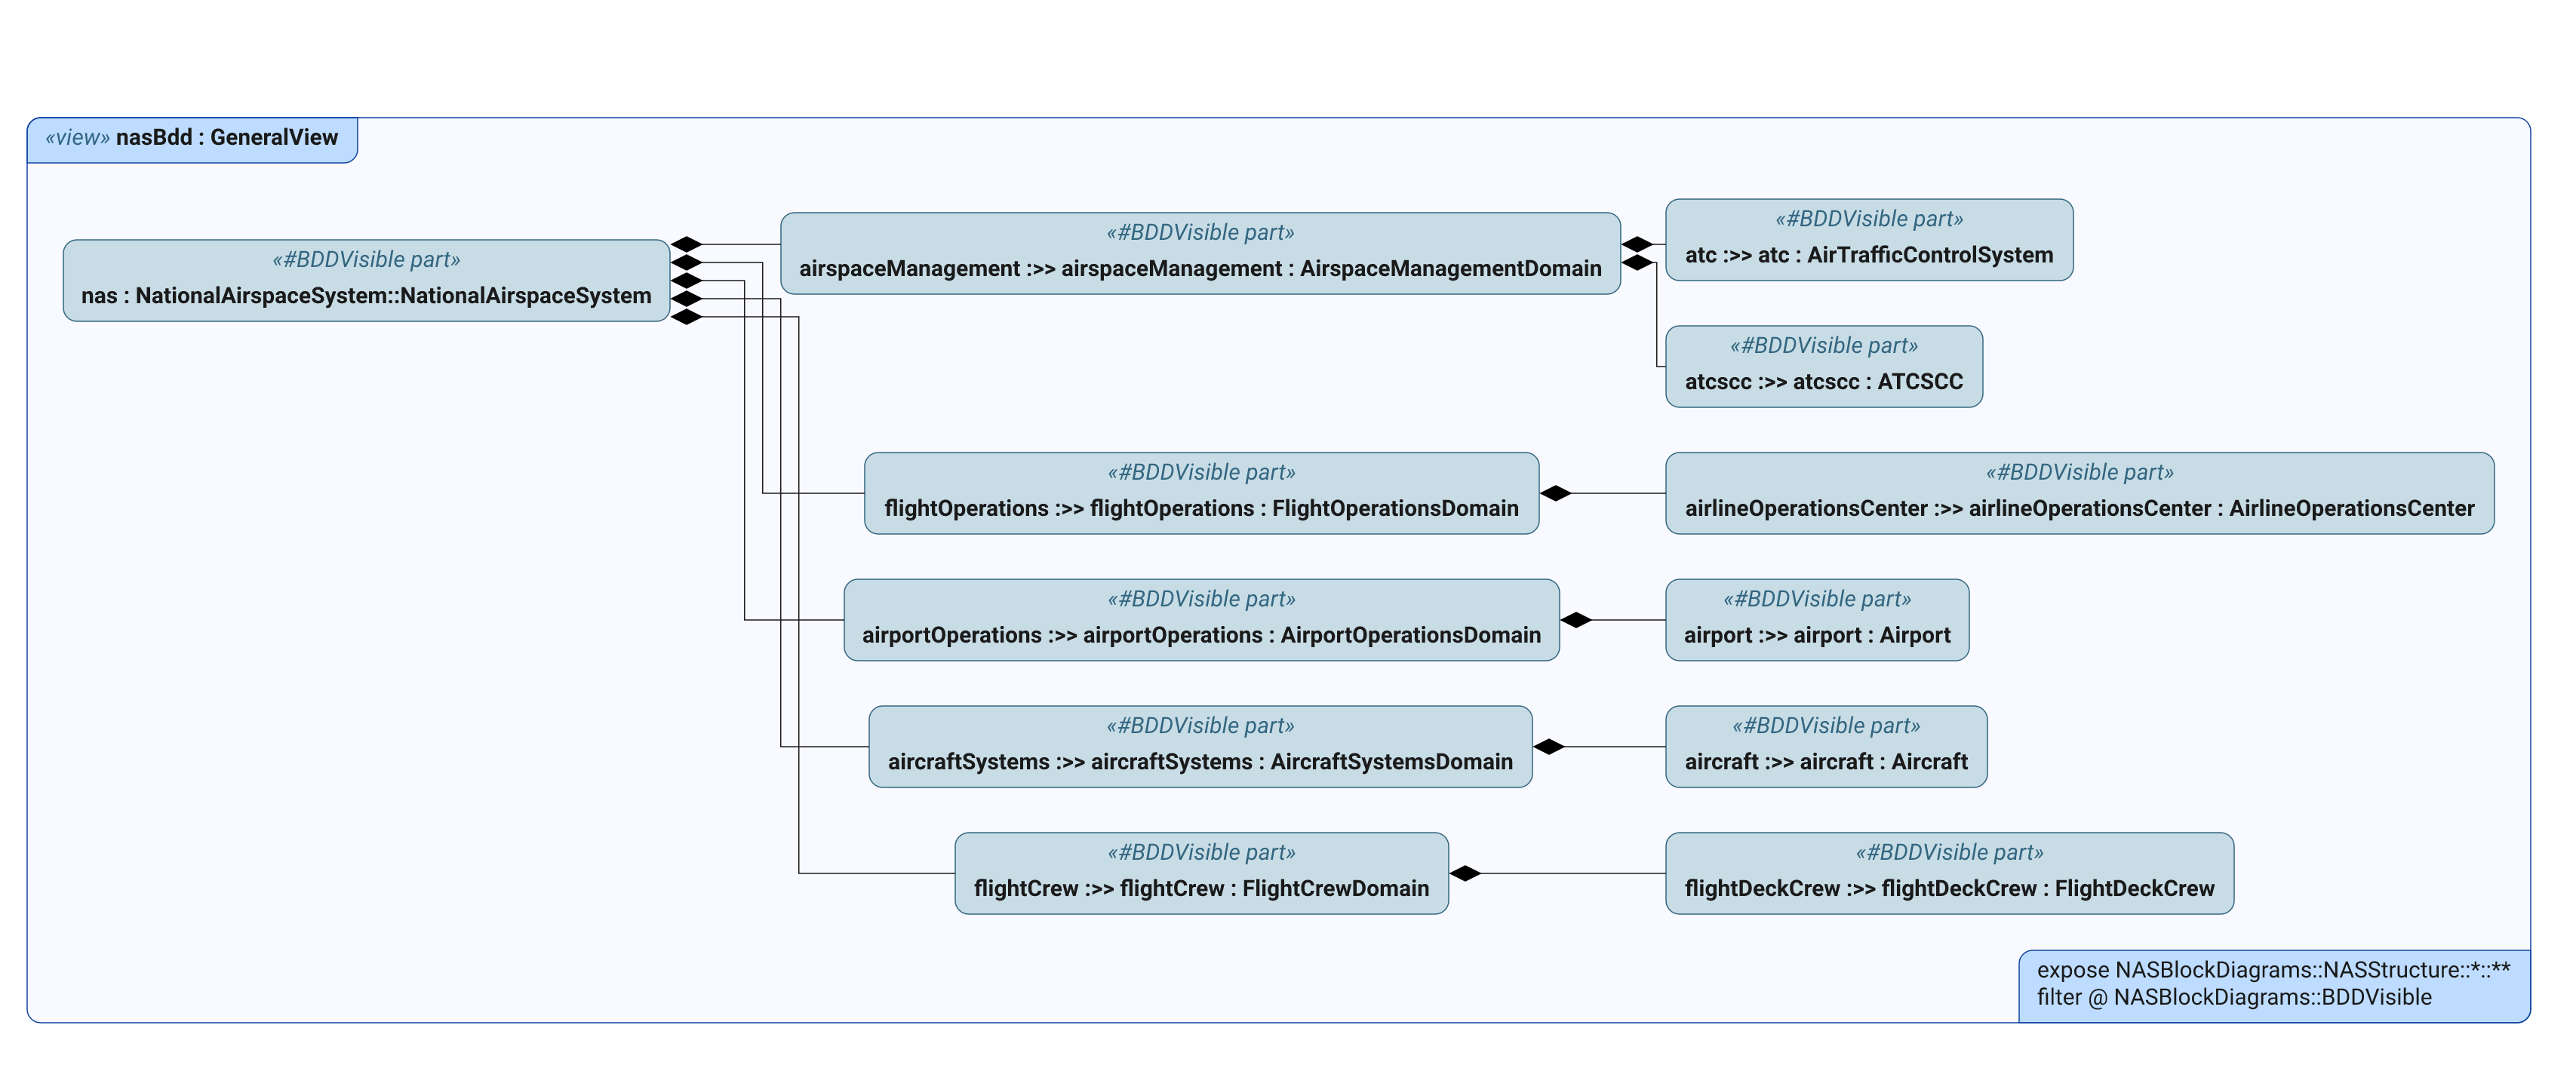
\includegraphics[width=\linewidth,height=0.8\textheight,keepaspectratio]{sysml/diagram-nasBdd}
\caption{NAS block definition diagram: the modeled domains and the context-diagram systems, composition only. View \texttt{nasBdd}; source \texttt{nas\_block\_diagrams.sysml}; rendered 2026-10-19.}
\label{fig:sysml-nasBdd}
\end{figure}
\end{landscape}

\begin{landscape}
\begin{figure}[!htbp]
\centering
\pdfimageresolution=300
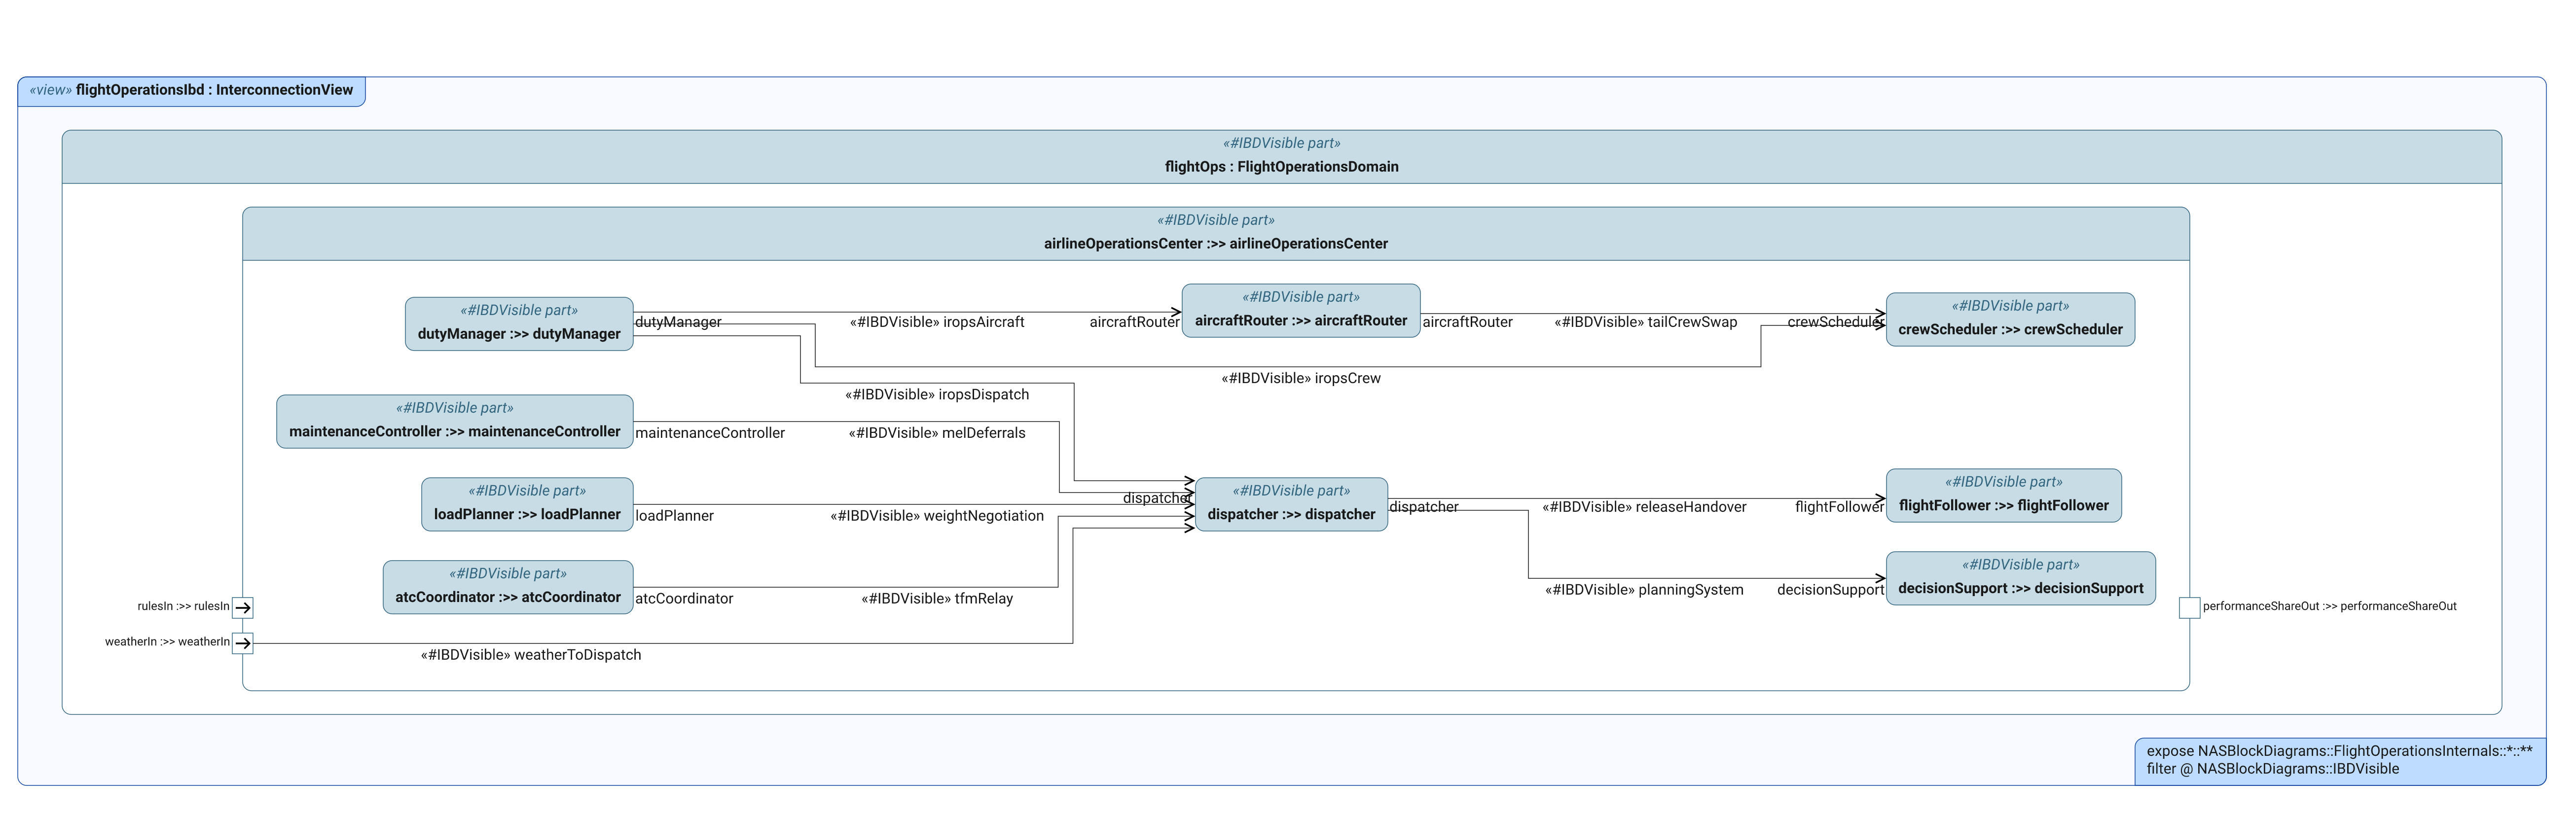
\includegraphics[width=\linewidth,height=0.8\textheight,keepaspectratio]{sysml/diagram-flightOperationsIbd}
\caption{Flight operations internal block diagram: the airline operations center's roles. View \texttt{flightOperationsIbd}; source \texttt{nas\_block\_diagrams.sysml}; rendered 2026-10-19.}
\label{fig:sysml-flightOperationsIbd}
\end{figure}
\end{landscape}

\begin{landscape}
\begin{figure}[!htbp]
\centering
\pdfimageresolution=300
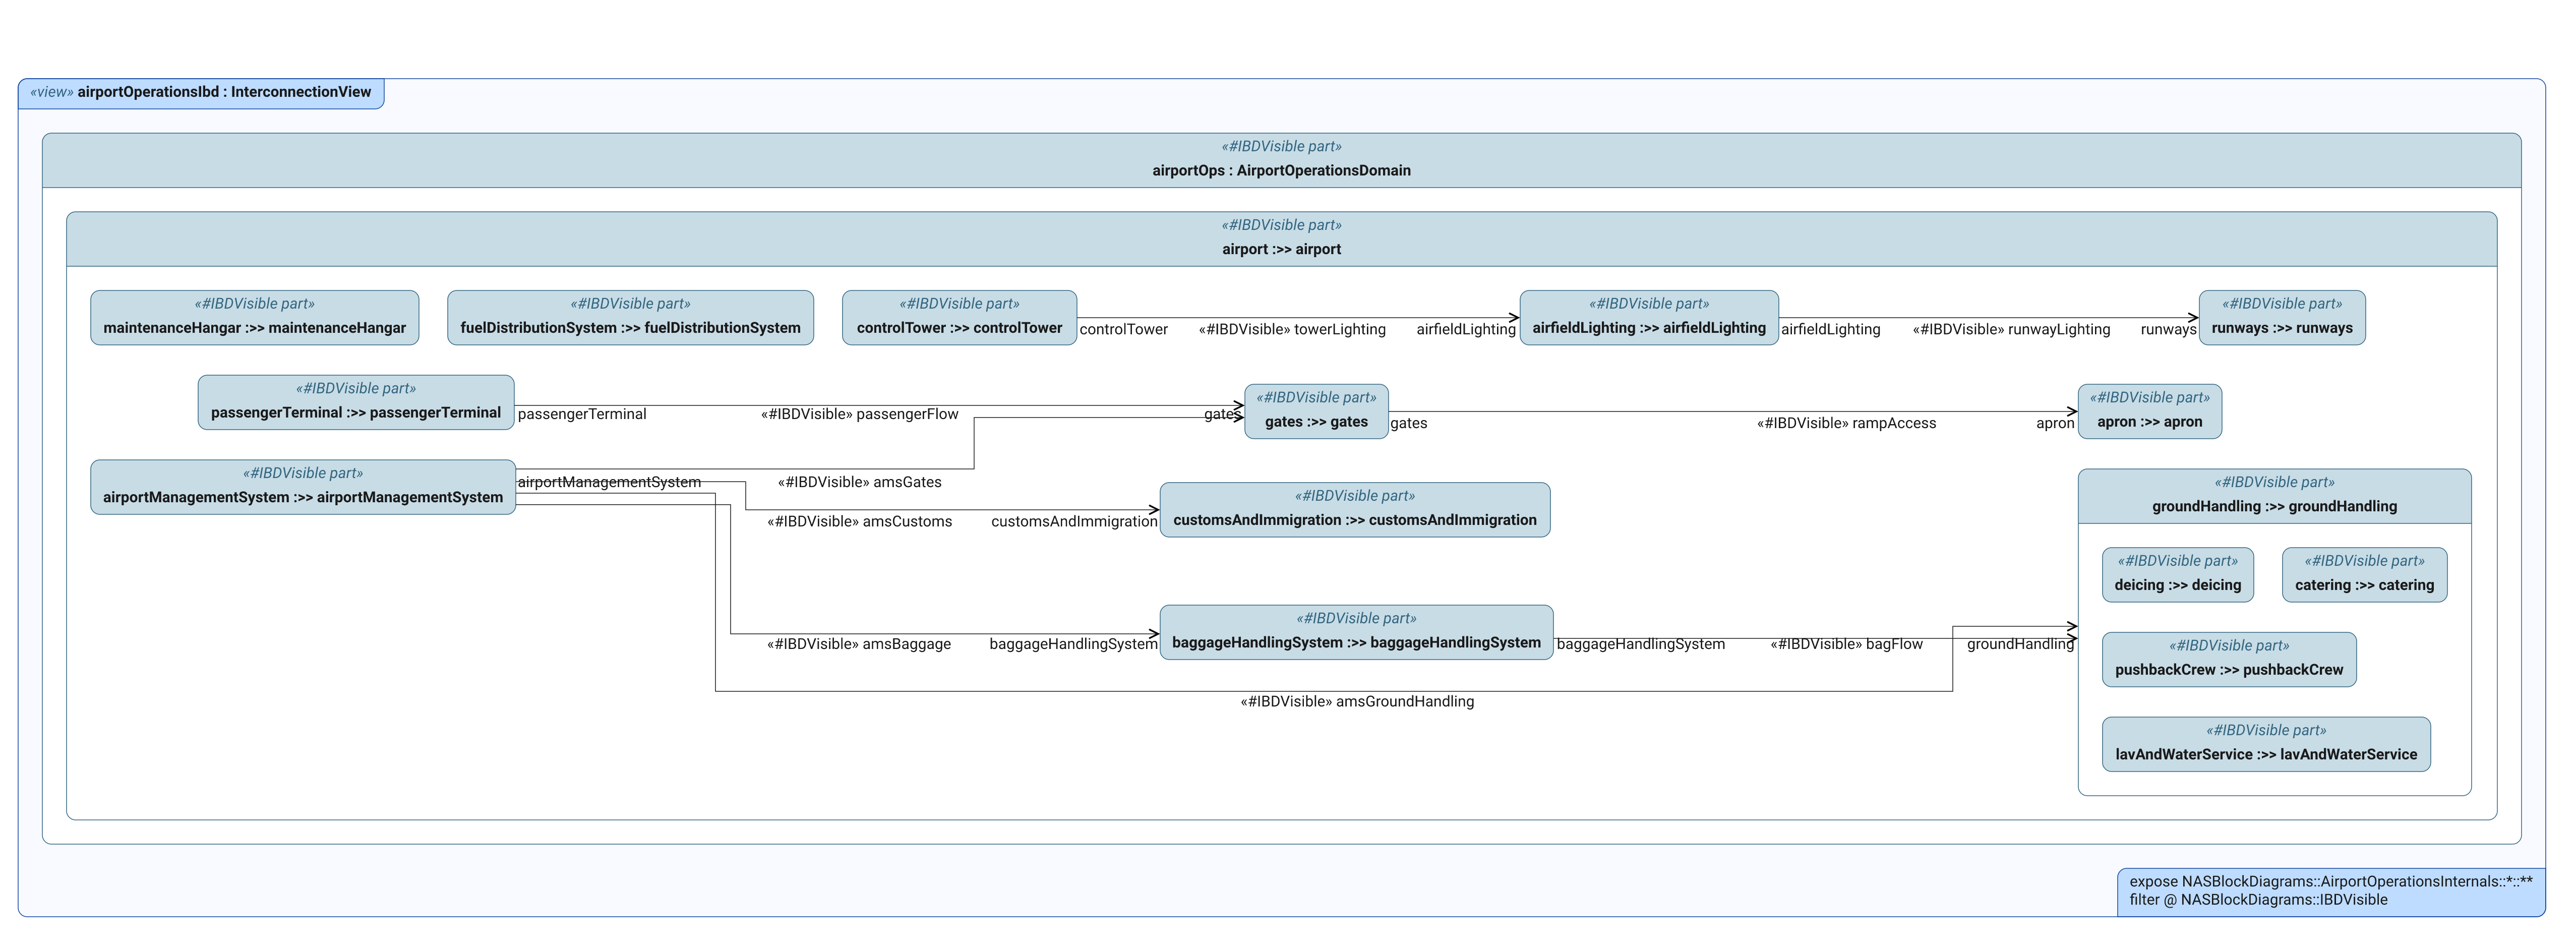
\includegraphics[width=\linewidth,height=0.8\textheight,keepaspectratio]{sysml/diagram-airportOperationsIbd}
\caption{Airport operations internal block diagram. View \texttt{airportOperationsIbd}; source \texttt{nas\_block\_diagrams.sysml}; rendered 2026-10-19.}
\label{fig:sysml-airportOperationsIbd}
\end{figure}
\end{landscape}

\begin{landscape}
\begin{figure}[!htbp]
\centering
\pdfimageresolution=300
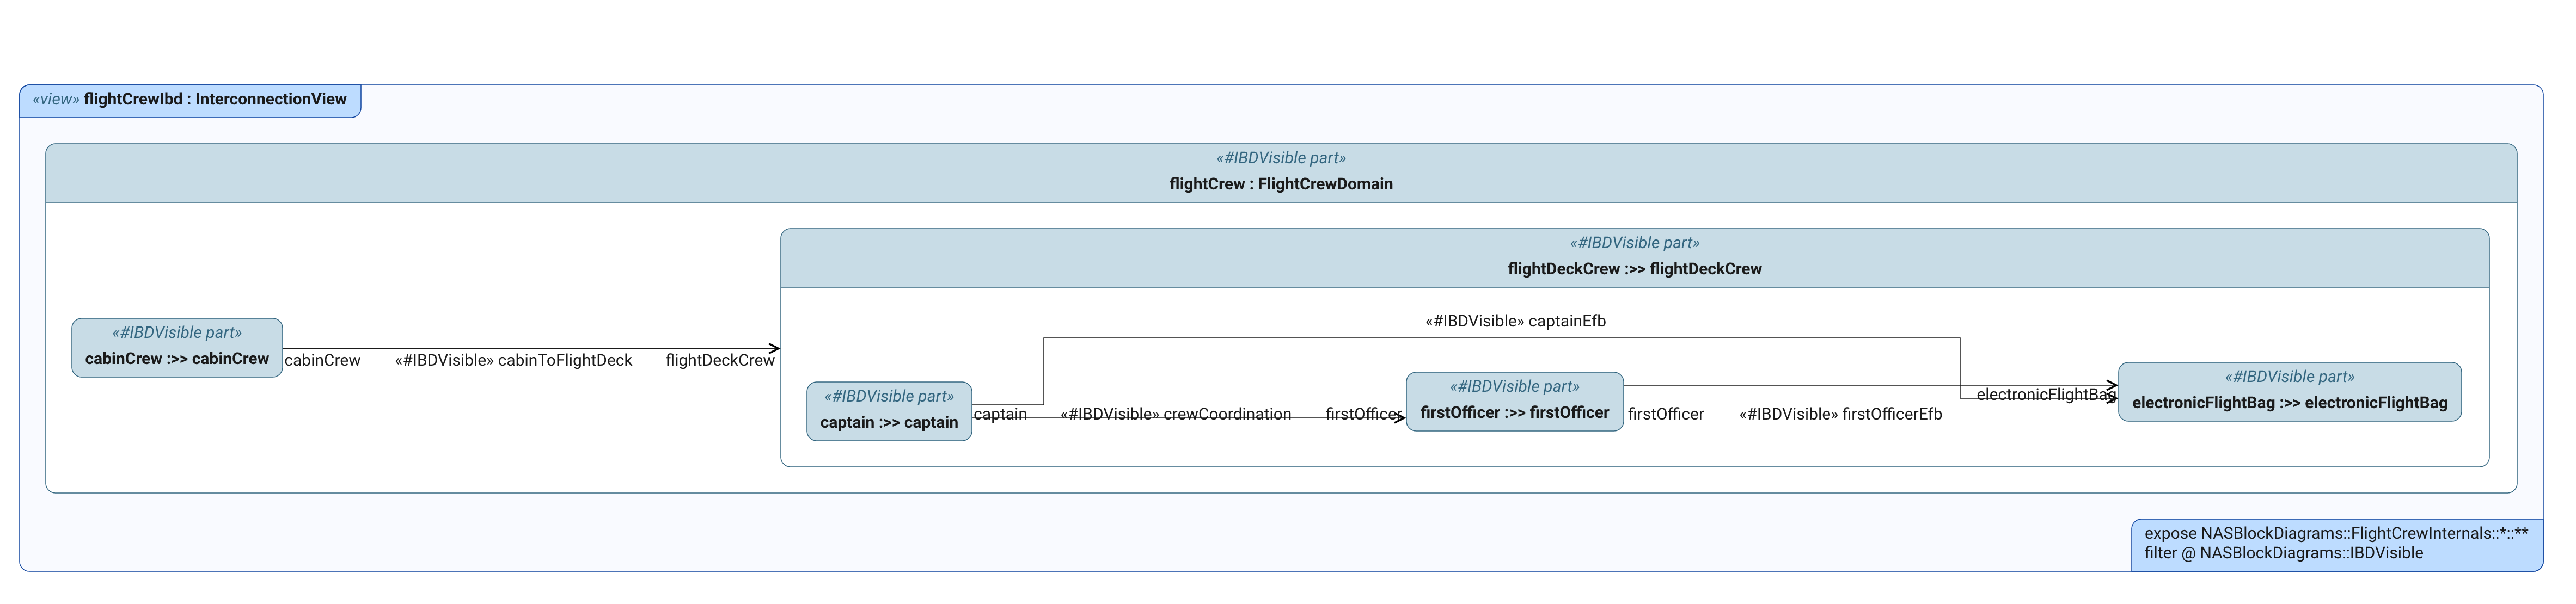
\includegraphics[width=\linewidth,height=0.8\textheight,keepaspectratio]{sysml/diagram-flightCrewIbd}
\caption{Flight crew internal block diagram. View \texttt{flightCrewIbd}; source \texttt{nas\_block\_diagrams.sysml}; rendered 2026-10-19.}
\label{fig:sysml-flightCrewIbd}
\end{figure}
\end{landscape}

\begin{landscape}
\begin{figure}[!htbp]
\centering
\pdfimageresolution=300
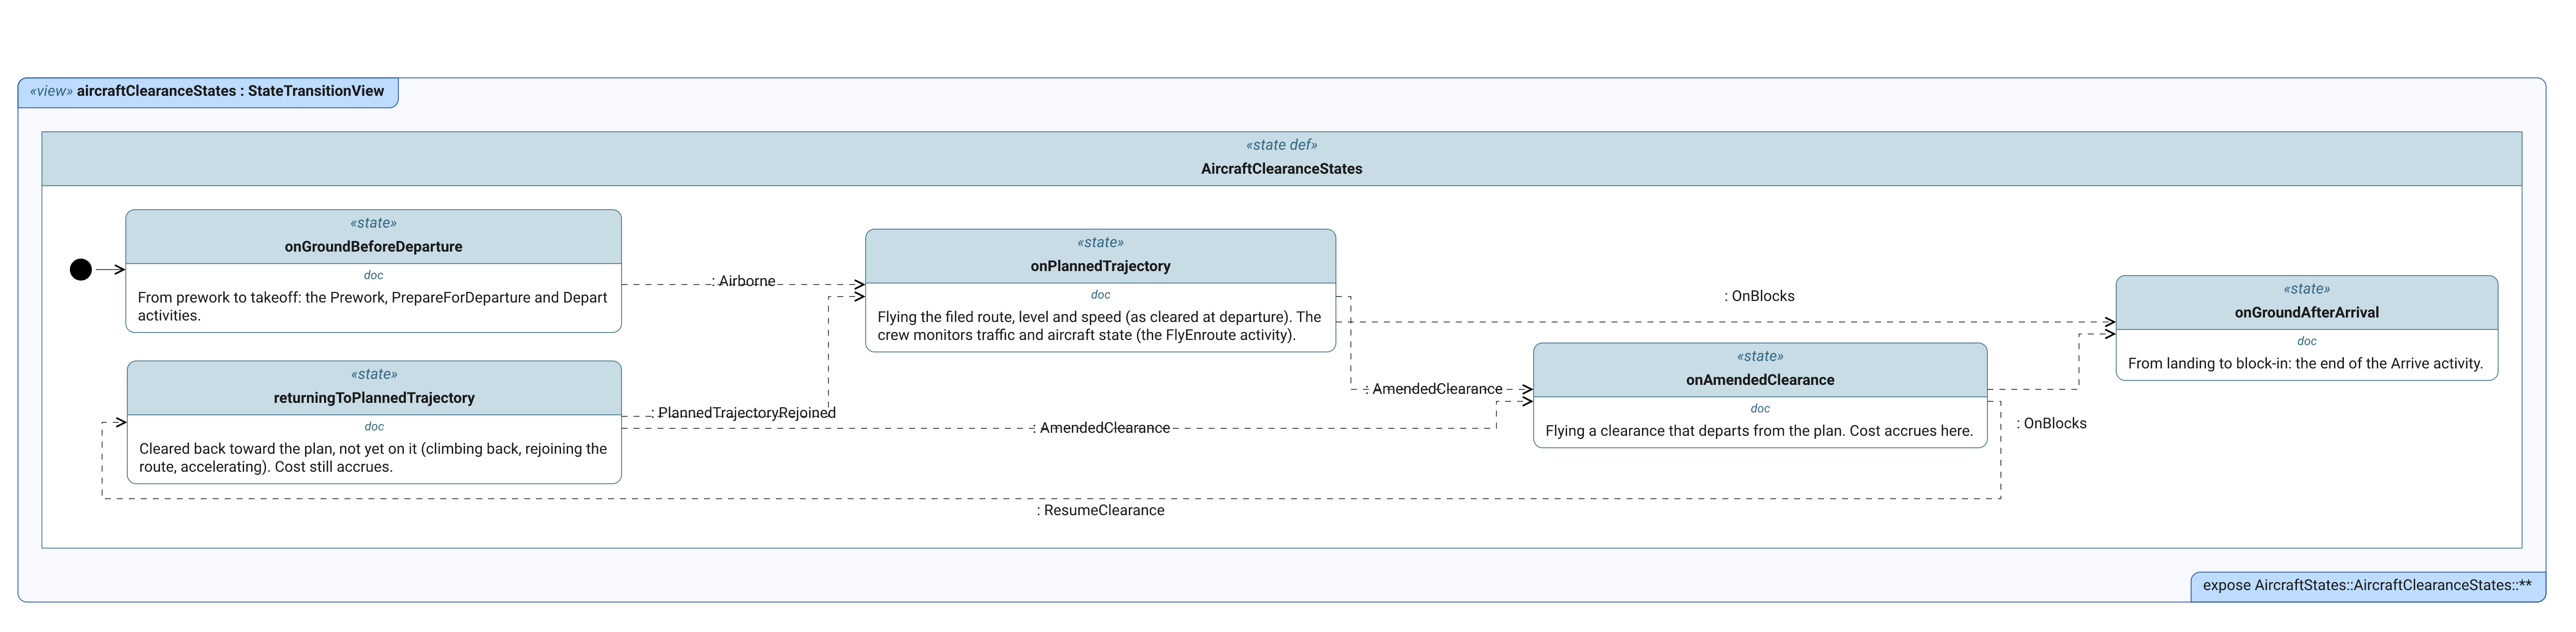
\includegraphics[width=\linewidth,height=0.8\textheight,keepaspectratio]{sysml/diagram-aircraftClearanceStates}
\caption{Aircraft state machine: the clearance the aircraft is flying, from the ground before departure to the ground after arrival. View \texttt{aircraftClearanceStates}; source \texttt{nas\_state\_aircraft.sysml}; rendered 2026-10-28.}
\label{fig:sysml-aircraftClearanceStates}
\end{figure}
\end{landscape}

\begin{landscape}
\begin{figure}[!htbp]
\centering
\pdfimageresolution=300
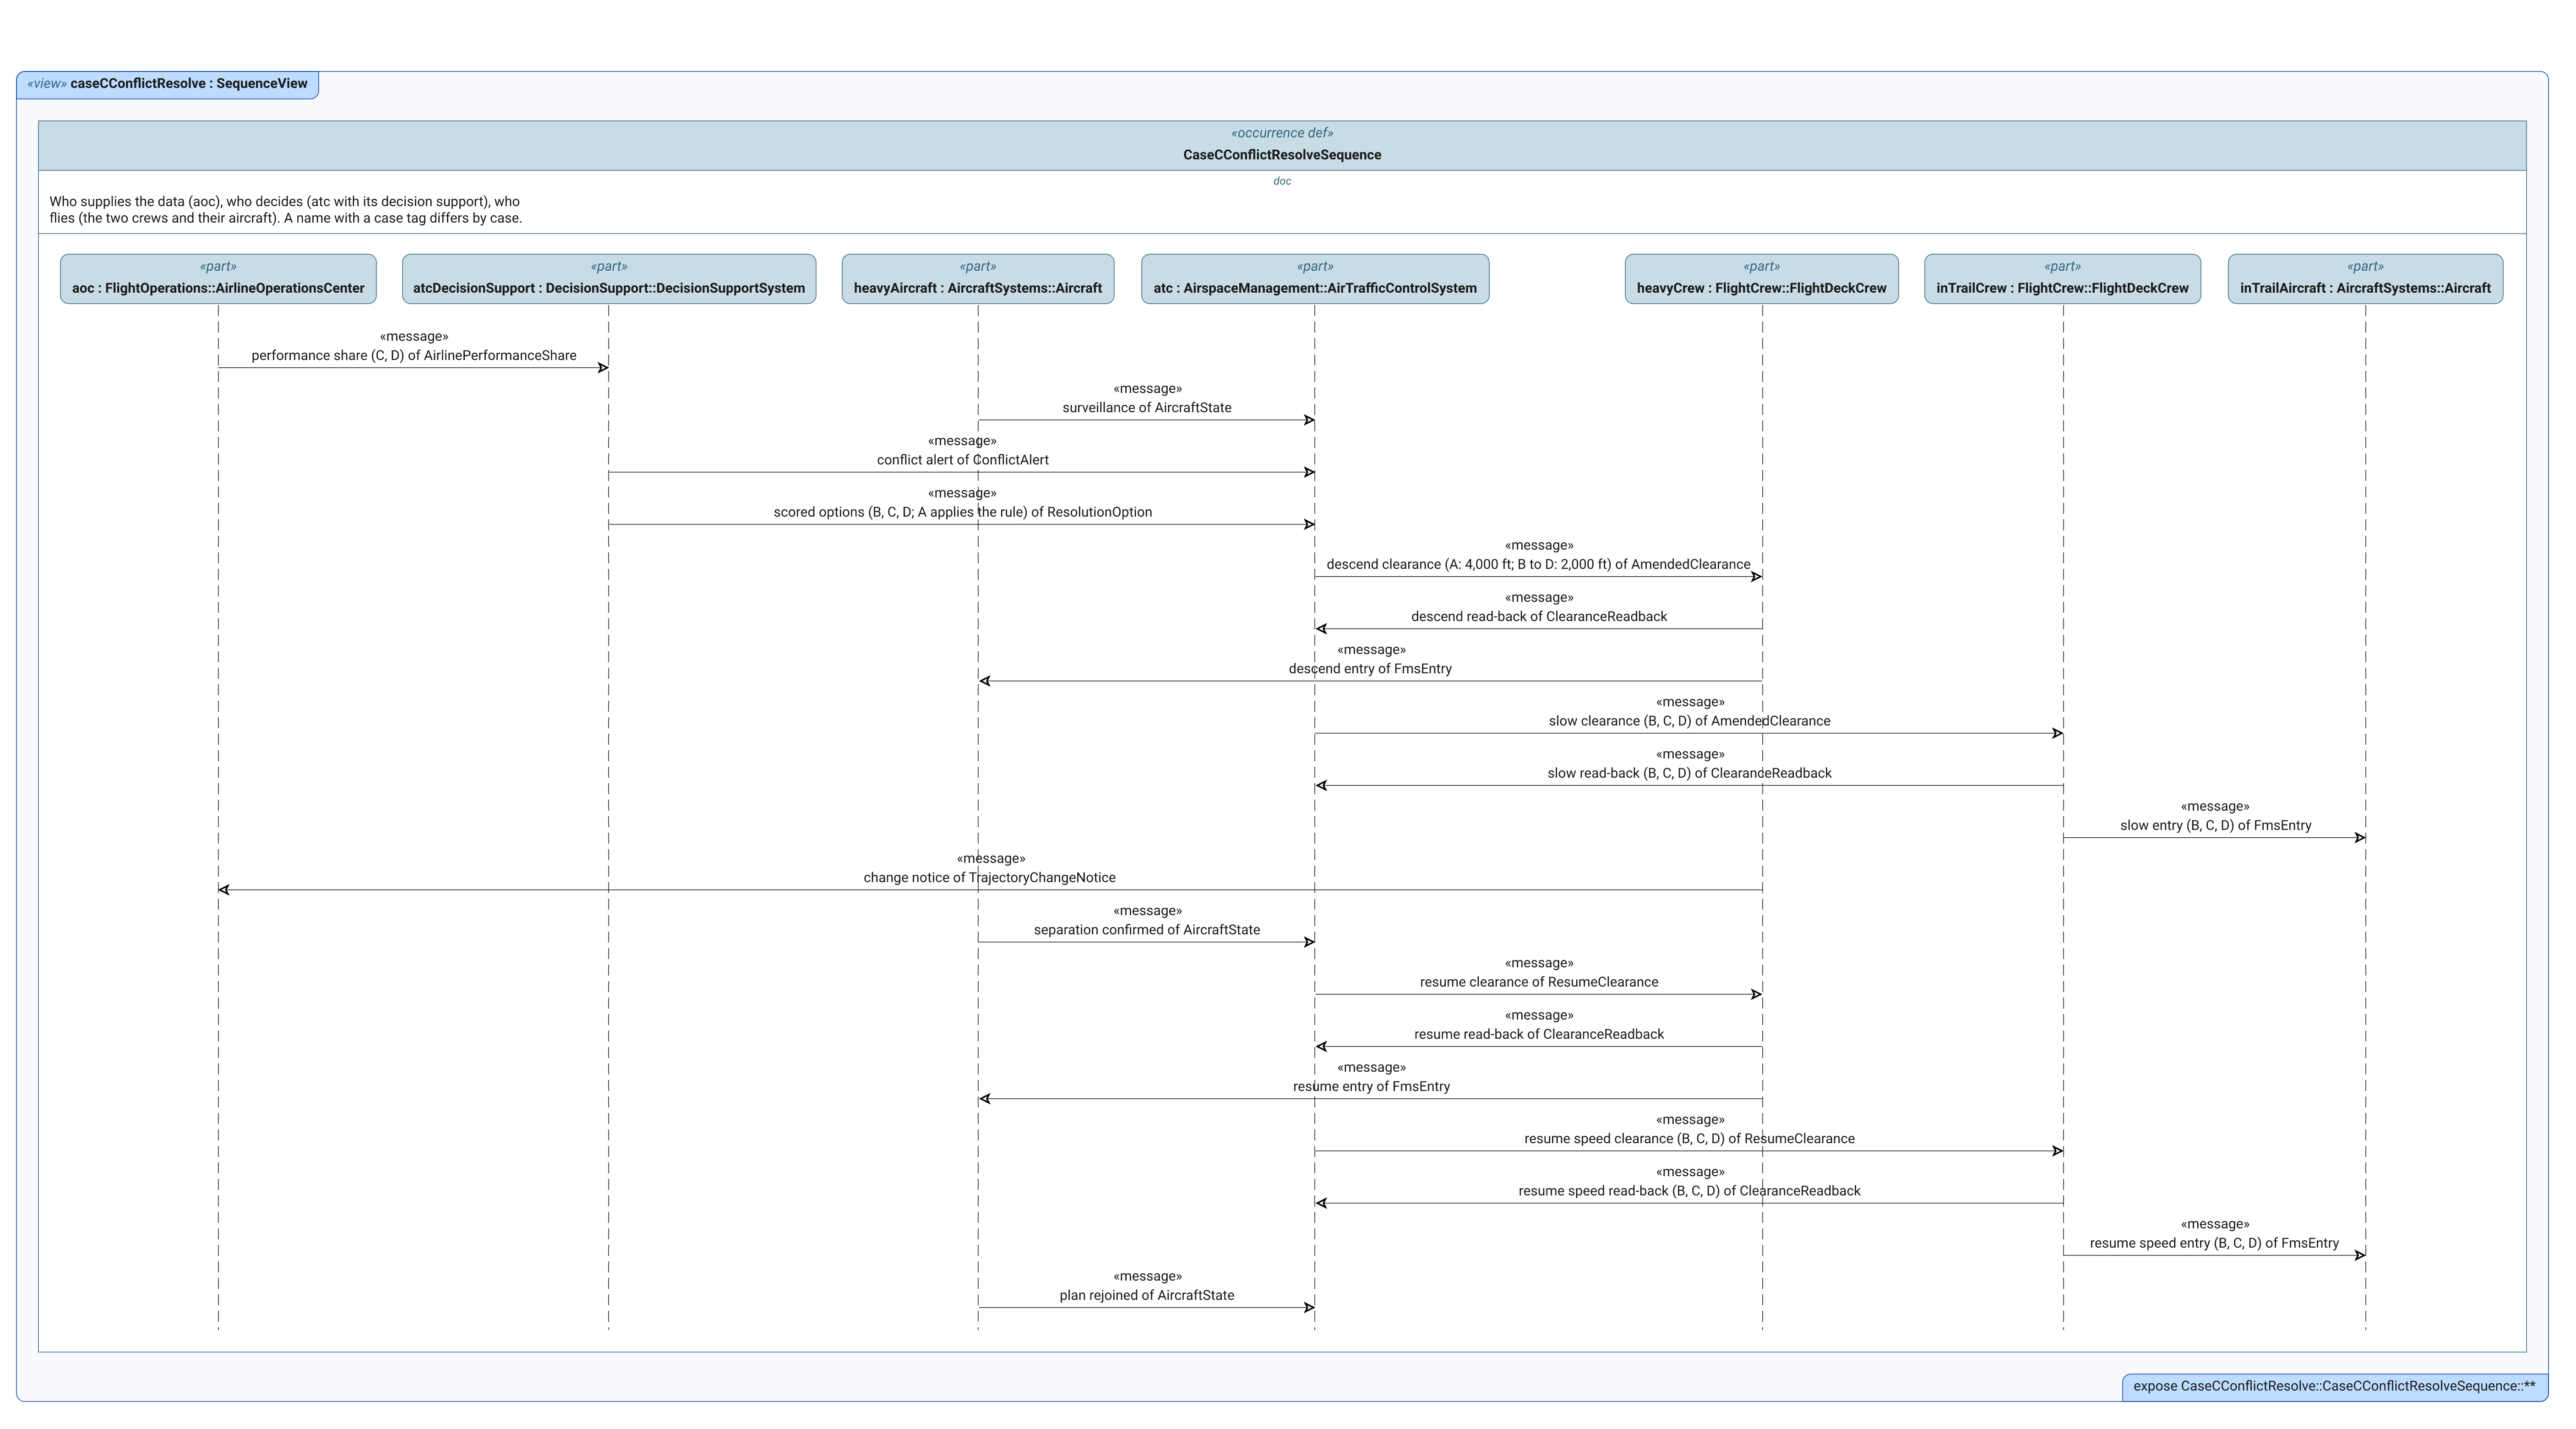
\includegraphics[width=\linewidth,height=0.8\textheight,keepaspectratio]{sysml/diagram-caseCConflictResolve}
\caption{Case C Conflict Resolve: the exchanges when ATC decision support scores the options with the airline's shared data. View \texttt{caseCConflictResolve}; source \texttt{nas\_sequence\_case\_c.sysml}; rendered 2026-10-28.}
\label{fig:sysml-caseCConflictResolve}
\end{figure}
\end{landscape}

\begin{landscape}
\begin{figure}[!htbp]
\centering
\pdfimageresolution=300
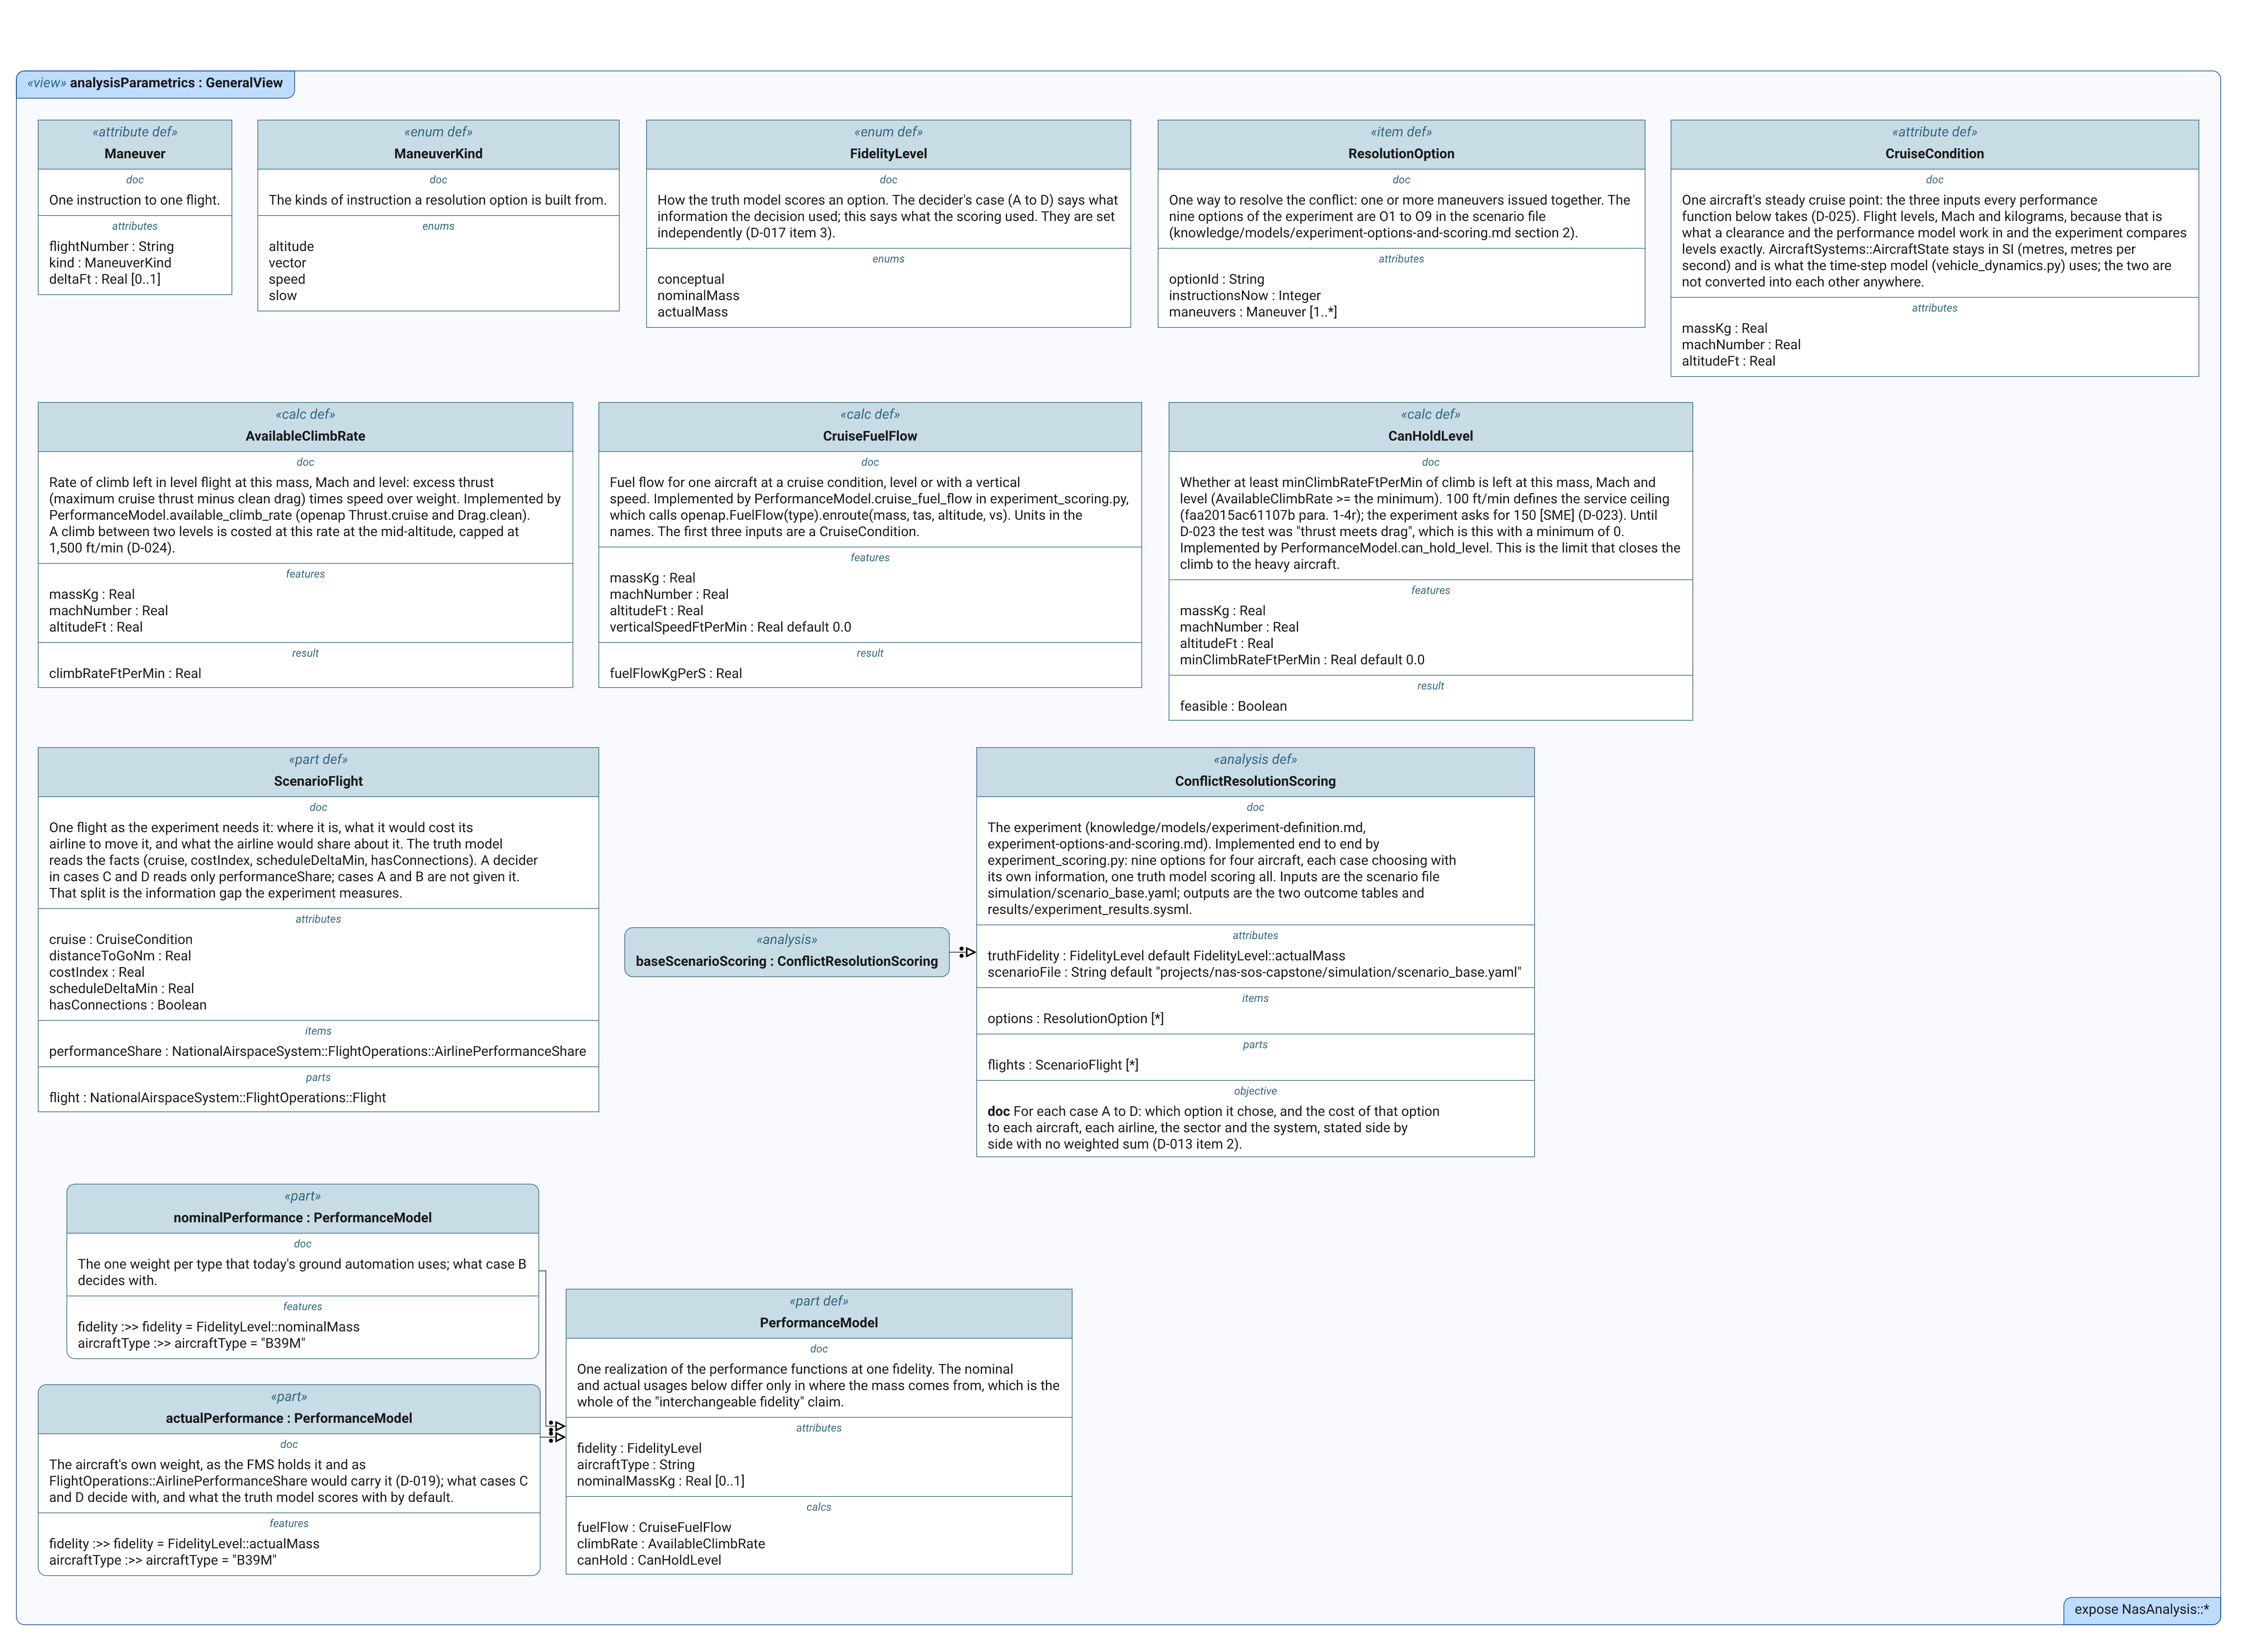
\includegraphics[width=\linewidth,height=0.8\textheight,keepaspectratio]{sysml/diagram-analysisParametrics}
\caption{Analysis definitions: the performance calculations, the two fidelity usages and the conflict-resolution scoring analysis. View \texttt{analysisParametrics}; source \texttt{nas\_analysis.sysml}; rendered 2026-10-28.}
\label{fig:sysml-analysisParametrics}
\end{figure}
\end{landscape}

% ---- end generated figures

\subsection{Full Myopic-Optimization Conflict Catalog}
\label{app:myopic}
\plantodo{S9}{All candidate conflicts not carried into the main-body
discussion or the S11--S14 demonstration scenario, each with: decision
maker, decision variable, local objective/constraints, affected
stakeholders, externalized costs, SoS consequence, and information needed
to recognize the consequence.}

\subsection{Optimization Experiment Detail}
\label{app:optimization}
\plantodo{S11, S12}{Full experiment matrix, constituent-model validation
notes, and any sensitivity-analysis detail not included in
Section~\ref{sec:results}.}

% ---- Placeholders added 2026-10-09 (AI-drafted scaffolding, not report prose).
\plantodo{S11}{Full options table: for each of the ten options, the
maneuver per aircraft, instructions now, follow-up later, and what the
decider must know to use it. Draft in
\texttt{knowledge/models/experiment-options-and-scoring.md} \S2.}

\plantodo{S11, S12}{Every option scored at four levels (the table from which
each case picks one row), the per-viewpoint cost statements with their
symbols defined, and the table of abstractions with reason and risk.}
% ---- end placeholders 2026-10-09

\subsection{Generative AI Use Disclosure}
\label{app:genai}

Generative AI was used as an assistant throughout this project. VS Code was the primary environment in which content was created, and the Claude Code extension (Anthropic) [cite] provided guidance, feedback, and draft content within it. Before that, two ChatGPT (OpenAI) [cite] conversations helped shape the project's direction. They were part of the reasoning that moved it from a trajectory-optimization study to the NAS modeled as a system of systems, with optimization as one capability inside the architecture. All AI-drafted content was reviewed and modified as needed to reflect my own views, understanding, and work.

Beyond drafting content, AI was used as a guide in three ways. It supported schedule and progress management against the course milestones. It gave technical guidance. And it critiqued the work, sometimes in deliberately demanding reviewer roles. AI gave initial reviews of all sources I identified and downloaded, to help me prioritize my own reading. After I read and marked up a source, AI extracted my markings and folded them into a library of sources and excerpts that I drew on while writing. As I wrote report sections, I asked AI for reviews, modifications, critiques, and relevant sources and excerpts.

The project's engineering content was produced the same way: AI drafted, and I reviewed, usually by hand, on paper. AI drafted much of the SysML v2 model text and the requirements, using my own work (leveraged from prior classes and authored as part of this project) as a starting point. I printed the diagrams and requirements, marked them up by hand, and AI transcribed my markings and applied them for me to check. The requirements show the effect. AI's first draft had 27 stakeholder and 53 system requirements. Over three hand reviews I struck, reworded, or wrote requirements until the set covered only what bears on the decision studied. Links in the model carry an evidence grade, so a reader can tell a link drawn from a published source or FAA order from one drawn from my industry experience or from general knowledge.

I formulated the experiment, both conceptually and in detail. AI drafted the code that implements it, runs it, and measures its outputs. AI also wrote the supporting scripts: rendering the model's diagrams, exporting the requirements, generating this report's requirement tables, and extracting annotations from PDFs. Every scenario value used in the report was set or confirmed by me. 

This disclosure is itself an example of the process. I wrote the first version. AI checked it against the project's decision log and journals and found what it left out: the ChatGPT conversations, the extent of the model and requirements drafting, and the transcription of my hand reviews. It then drafted this revision, which I edited. As with the rest of the work, the check against the record was the useful part, and the final wording is mine.

\subsection{Source Register}
\label{app:sources}
\plantodo{S1--S4}{Reference or reproduce the evidence/source register
(\texttt{evidence/source-register.md}): source, publication type,
NAS lifecycle phase, systems/stakeholders addressed, architectural and
optimization evidence extracted, and confidence/limitations.}


\end{document}
